%%%%%%%%%%%%%%%%%%%%%%%%%%%%%%%%%%%%%%%%%%%%%%%%%%

% Latex Kapitel erstellen. 
% 		Kopiere 'texPandoc/*.tex' nach 'content/tex' 
% 		'content/tex' **Handarbeit... für opt. Ergebnisse!** 
% 		Kopiere 'archiv/inhalt.tex' nach 'content/' 
% 		make -- Latex-PDF erstellen 
% ju 17-Jul-2022 inhalt.tex

%%%%%%%%%%%%%%%%%%%%%%%%%%%%%%%%%%%%%%%%%%%%%%%%%%

% content/

\chapter{01-Kostenrechnung}
%%ju 28-Mai-22 01-Kostenrechnung.tex
$\to$ \emph{Ziel:} Kenngrößen verbessern (Produktivität,
Wirtschaftlichkeit, Umsatzrentabilität)

\textbf{Kosten- und Leistungsrechnung} (KLR) $\to$ internes
Rechnungswesen

vs.

\textbf{Buchhaltung} (FiBu) $\to$ externes Rechnungswesen

\textbf{Kosten einteilen}

\begin{enumerate}
\item
  \textbf{Vollkostenrechnung}

  \begin{itemize}
  \item
    Indirekte Kosten (Gemeinkosten, kalkulatorische Kosten)
  \item
    Direkte Kosten (Einzelkosten)
  \end{itemize}
\item
  \textbf{Kostenstellenrechnung} (Verursachergerechte Verteilung der
  Kosten: Lager, Werkstatt, Vertrieb)
\item
  \textbf{Teilkostenrechnung} (fixe Kosten, variable Kosten,
  Deckungsbeitrag)
\end{enumerate}

\section{Vollkostenrechnung}\label{vollkostenrechnung}

Vgl. Kostenrechnung Fachbuch S. 79-102
(\textcite{heiser:2017:betriebsfuhrung}).

\subsection{Kosten der Werkstatt}\label{kosten-der-werkstatt}

\begin{figure}[!ht]% hier: !ht
\centering
\includegraphics[width=0.4\textwidth]{images/Skizze/02_Umsatzerloese_Skizze.pdf}
\caption{Kosten und Erlöse}
%\label{fig:}%% anpassen
\end{figure}

\begin{enumerate}
\item
  \textbf{Einzelkosten} (EK), direkte Kosten (Kunden), Fertigungslöhne
  $\to$ produktive Löhne

  \begin{itemize}
  \item
    \emph{Beispiel:} Fertigungslöhne, Anschaffungskosten,
    Fertigungsmaterialien (Ersatzteile)
  \item
    $\boxed{\text{FL} = WSL \cdot Flh}$\\
  \item
    (WSL) = (StLs) Werkstattschnittlohn = Stundenlohnsatz
  \end{itemize}
\item
  \textbf{Gemeinkosten} (GK), indirekte Kosten, Hilfslöhne (W-Aufträge)
  $\to$ unproduktive Löhne

  \begin{itemize}
  \item
    $\boxed{\text{GK} = Seko - EK} \quad \boxed{\text{GK} = \frac{WSL \cdot GKZs}{100}}$
  \end{itemize}
\item
  \textbf{Selbstkosten} (SeKo)

  \begin{itemize}
  \item
    $\boxed{SeKo = EK + GK}$ (Einzelkosten + Gemeinkosten)
  \item
    $\boxed{SeKo = FL + GK}$ vs.~$\boxed{SeKo/h = WSL + GK/h}$
  \item
    $\boxed{SeKo_{EUR} = UE - GW} \to \boxed{SeKo_\% = 100~\% - UR_\%}$
  \end{itemize}
\item
  \textbf{Gewinn} (GW) in €

  \begin{itemize}
  \item
    $\boxed{\text{Gewinn} = UE - EK - GK} \quad \boxed{\text{Gewinn/h} = StVs - Seko/h}$
  \end{itemize}
\item
  \textbf{Umsatzerlöse} (UE in EUR), Stundenverrechnungssatz (StVs in
  EUR/h)

  \begin{itemize}
  \item
    Betrag für eine Leistung = Kostendecken + Gewinn
  \item
    $\boxed{UE = EK + GK + GW} \quad \boxed{UE = Seko + GW}$
    (Selbstkosten + Gewinn)
  \item
    $\boxed{StVs = StLs/WSL + GK + GW}$
  \end{itemize}
\end{enumerate}

\subsection{Gemeinkosten}\label{gemeinkosten}

\emph{Beispiel:}

\begin{itemize}
\item
  Lohn+Gehalt (unproduktiv)
\item
  Reisekosten
\item
  Kfz (geschäftlich)
\item
  Afa
\item
  Eigenkapital (EK \% Zins)
\item
  kalkulatorische Pacht
\item
  Meisterlohn (unproduktiv)
\item
  kalkulatorische Lohn (Frau)
\end{itemize}

\begin{enumerate}
\item
  \textbf{Gemeinkostenzuschlagsatz} (GKZs) in \%

  \begin{itemize}
  \item
    $\boxed{\text{GKZs} = \frac{GK \cdot 100}{FL}}$
  \end{itemize}
\item
  \textbf{Kalkulatorische Kosten} Gemeinkosten, die keine Ausgaben
  verursachen; aufwandsfremde Kosten

  \begin{itemize}
  \item
    \emph{Beispiel:} kalk.-Miete, kalk.-Abschreibungen, kalk.-Zinsen,
    kalk.-U-Lohn, kalk.-Wagnisse
  \end{itemize}
\item
  \textbf{Hilfslöhne} entstehen bei Werkstattaufträgen (W-Aufträge)

  \begin{itemize}
  \item
    \emph{Beispiel:} Leerlauf, Nacharbeiten, Reparatur von
    Werkstattfahrzeuge, Urlaub, Feiertage, Wartezeiten
  \end{itemize}
\end{enumerate}

\subsection{Gewinn}\label{gewinn}

Einkommen des Unternehmers, Wagnis, Unternehmensrisiko

\textbf{Gewinnzuschlag} (GWZs) in \%
$\boxed{\text{GWZs} = \frac{GW \cdot 100}{SeKo}}$

\newpage

\subsection{Fertigungslöhne}\label{fertigungsloehne}

\begin{enumerate}
\item
  \textbf{Fertigungslöhne} (FL), >>produktiv<<, EK, direkt

  \begin{itemize}
  \item
    Auftrag direkt dem Kunden in Rechnung stellen
  \item
    $\boxed{\text{FL} = WSL \cdot Flh}$
  \item
    \emph{Beispiel:} $90~\%$ Lohnkosten
  \end{itemize}
\end{enumerate}

$+$

\begin{enumerate}
\setcounter{enumi}{1}
\item
  \textbf{Hilfslöhne} (HL) >>unproduktiv<<, GK, nicht direkt

  \begin{itemize}
  \item
    \emph{Beispiel:} $10~\%$ Lohnkosten
  \end{itemize}
\end{enumerate}

$= 100~\%$

\textbf{Fertigungslöhne entstehen bei}

\begin{enumerate}
\item
  \textbf{K-Aufträge}

  \begin{itemize}
  \item
    Kundenauftrag, externe Aufträge
  \item
    \emph{Beispiel:} Wartung, Kundendienst, Reparatur
  \end{itemize}
\item
  \textbf{I-Aufträge}

  \begin{itemize}
  \item
    interne Aufträge, innerbetrieblich (andere Abteilung des Betriebs)
  \item
    \emph{Beispiel:} Fahrzeugaufbereitung, Gebrauchtwagenreparatur,
    Überführung, Übergabedurchsicht
  \end{itemize}
\item
  \textbf{G+K-Aufträge}

  \begin{itemize}
  \item
    Garantie- und Kulanzanträge
  \item
    für Kunden ohne Berechnung, Gründe: Kulanz, Sachmängelhaftung,
    Kundenzufriedenheit gewährleisten
  \end{itemize}
\end{enumerate}

\newpage

\textbf{Zeitlohn vs.~Leistungslohn}

\begin{enumerate}
\item
  \textbf{Zeitlohn} Fertigungslohn, produktive Arbeitszeit, Stundenlohn,
  Tariflohn

  \begin{itemize}
  \item
    \textbf{FLh} Fertigungslohnstunden
  \item
    \textbf{WSL} Werkstattschnittlohn, quer durch die Werkstatt
    \emph{Beispiel:} Lehrling, Geselle

    \begin{itemize}
    \item
      $\boxed{\text{WSL} = \frac{FL}{Flh}}$
    \end{itemize}
  \end{itemize}
\item
  \textbf{Leistungslohn} Lohn für die erbrachte Leistung

  \begin{itemize}
  \item
    \textbf{AWLs} Arbeitswertlohnsatz
  \item
    \textbf{ZELs} Zeiteinheitenlohnsatz
  \item
    \textbf{Soll-AW} Vorgabe, wie viele AW muss ich in einer Stunde
    machen?
  \item
    \textbf{Ist-AW} tatsächlich erbrachte Leistung
  \item
    \textbf{Mehr-AW} Mehrleistung in AW
    $\boxed{\text{AW} = \text{Ist-AW} - \text{Soll-AW}}$
  \item
    \textbf{Vorgabezeiten} Grundlage für Leistungslohn

    \begin{itemize}
    \item
      \textbf{ZE} Zeiteinheit (in Min.)
    \item
      (StVs / 60 = €/ZE x Min. = Preis (€))
    \item
      \textbf{AW} Arbeitswert (in Min.) Richtzeiten, Vorgabezeiten
    \item
      \textbf{WF} Werkstattfaktor $\to$ wie viele AW/ZE in einer
      Stunde? (Soll-Leistung, Mindestleistung) (12 AW/h =
      $\frac{60}{12}$ alle 5 Min. 1 AW)
    \item
      \textbf{Leistungsfaktor} (LF) Ist-Leistung

      \begin{itemize}
      \item
        tatsächlich erbrachte Leistung je Stunde
      \item
        Leistungsfaktor = Ist-Leistung in AW / Fertigungslohnstunden
      \item
        LF = Ist-AW / FLh
      \end{itemize}
    \item
      \textbf{Leistungsgrad} (LG)

      \begin{itemize}
      \item
        $\boxed{\text{LG} = \frac{\text{Ist-AW}}{\text{Soll-AW}}}$
      \item
        (Ist-Leistung / Soll-Leistung) und (tatsächlich erbrachte
        Leistung / Mindestleistung)
      \end{itemize}
    \item
      \textbf{Leistungslohnsatz}

      \begin{itemize}
      \item
        Leistungslohnsatz = Fertigungslohn / Fertigungslohnstunden
      \item
        LLs = FL / FLh
      \end{itemize}
    \end{itemize}
  \end{itemize}
\end{enumerate}

\newpage

\subsection{Kennwerte der Werkstatt}\label{kennwerte-der-werkstatt}

\begin{enumerate}
\item
  \textbf{Soll-Umsatzerlös} (Soll-UE) deckt die Selbstkosten ab

  \begin{itemize}
  \item
    Soll-UE = Seko + GW
  \end{itemize}
\item
  \textbf{Ist-Umsatzerlös} tatsächlich erwirtschaftete Umsatz
\item
  \textbf{Lohnerlöse} Umsatzerlöse
\item
  \textbf{Wirtschaftlichkeit} (WI) wurde Gewinn oder Verlust gemacht
  \emph{Beispiel:} 1,05 \% $\to$ 5 \% mehr

  \begin{itemize}
  \item
    Wirtschaftlichkeit = Umsatzerlöse / Selbstkosten
  \item
    WI = LE / Seko; WI = UE/Seko
  \item
    WI > 1 Gewinn
  \item
    WI \textless{} 1 Verlust
  \item
    WI = 1 Kostendeckend
  \end{itemize}
\item
  \textbf{Produktivität} (PR)

  \begin{itemize}
  \item
    Gesamte Arbeitszeit (Fertigungs- + Hilfslohnstunden)
  \item
    Produktivität = Fertigungslohnstunden x 100 / Arbeitszeit
  \item
    PR = FLh x 100 / AZ
  \end{itemize}
\item
  \textbf{Umsatzrentabilität} (UR) in \%

  \begin{itemize}
  \item
    Wie viel Prozent des Umsatzes als Gewinn anfallen
  \item
    $\boxed{\text{UR} = \frac{GW \cdot 100}{UE}} \quad \boxed{\text{UR} = \frac{GW/h \cdot 100}{StVs}}$
  \end{itemize}
\end{enumerate}

\newpage

\subsubsection{Kostenindex - Stundenverrechnungssatz - AW-Vs
(Prüfung)}\label{kostenindex-stundenverrechnungssatz-aw-vs-pruefung}

\emph{3x wichtige Formeln}

\textbf{Kostenindex, Werkstattindex, Faktor} (KI) wievielmal mehr der
Kunde für eine Fertigungslohnstunde zu bezahlen hat, als der Monteur in
dieser Stunde verdient. (bezieht sich auf Löhne)

$\boxed{\text{KI} = \frac{\text{Prod. Löhne} + \text{GK} + \text{Gewinn}}{\text{Prod. Löhne}}} \quad \boxed{\text{KI} = \frac{\text{FL} + \text{GK} + \text{GW}}{\text{FL}}} \quad$
$\boxed{\text{KI} = \frac{\text{StVs}}{\text{WSL}}} \quad \boxed{\text{KI} = \frac{\text{UE}}{\text{FL}}}$

\textbf{Stundenverrechnungssatz} Arbeitspreis, der dem Kunden für eine
Stunde berechnet wird. Reparaturstunde = Fertigungslohnstunde

$\boxed{\text{StVs} = \frac{\text{UE}}{\text{FLh}}} \quad \boxed{\text{StVs} = \text{KI} \cdot \text{WSL}}$

$\boxed{\text{StVs}_{neu} = \frac{\text{Seko}_{neu} \cdot 100~\%}{\text{Seko}_{alt}}} \quad \boxed{\Delta \text{StVs} = \text{StVs}_{neu} - \text{StVs}_{alt}}$

Erhöhung
$\boxed{\text{StVs}_\% = \frac{\Delta \text{StVs} \cdot 100~\%}{\text{StVs}_{alt}}}$

\textbf{AW-Verrechnungssatz} Ermittlung des Arbeitspreises für eine
Arbeitsposition (Leistungslohn)

Erlös je AW

$\boxed{\text{AW-Vs} = \frac{\text{StVs}}{\text{WF}}} \quad \boxed{\text{AW-Vs} = \frac{\text{WSL} \cdot \text{KI}}{\text{WF}}} \quad \boxed{\text{AW-Vs} = \frac{\text{UE}}{\text{FLh} \cdot \text{WF}}}$

\newpage

\subsection{Handelswarenkalkulation}\label{handelswarenkalkulation}

\textbf{Kalkulationsarten} Vorwärts-, Rückwärts-, Differenzkalkulation

\subsubsection{Einkaufskalkulation}\label{einkaufskalkulation}

\lstset{language=Python}% C, TeX, Bash, Python 
\begin{lstlisting}[
	%caption={}, label={code:}%% anpassen
]
  BP                                           LEP                 // 100 %
- BK                                         - Rabatt       10 %                 
= BEP                           // 98 %      = ZEP                 // 100 % 
+ Skonto    2 % (in 100)                     - Skonto        2 %
= ZEP                           // 90 %      = BEP                 
+ Rabatt   10 % (in 100)                     + BK
________________________________             ______________________         
= LEP                           EUR          = BP                  EUR 
\end{lstlisting}

\begin{enumerate}
\item
  \textbf{Listeneinkaufspreis} (LEP), Ware, Angebot,
  $\boxed{BEP + \text{Skonto} + \text{Rabatt}}$
\item
  \textbf{Lieferantenrabatt} (LRa), Preisnachlass
\item
  \textbf{Zieleinkaufspreis} (ZEP), Zahlungszeitpunkt, Kauf auf Ziel
  $\boxed{BEP + \text{Skonto}}$
\item
  \textbf{Lieferantenskonto} (LSk)
\item
  \textbf{Bareinkaufspreis} (BEP), bei sofortiger Barzahlung
\item
  \textbf{Bezugskosten} (BK), Transport: Verpackung, Fracht, Zoll,
  Rollgeld
\end{enumerate}

\subsubsection{Verkaufskalkulation,
Ersatzteilkalkulation}\label{verkaufskalkulation-ersatzteilkalkulation}

\lstset{language=Python}% C, TeX, Bash, Python 
\begin{lstlisting}[
	%caption={}, label={code:}%% anpassen
]
  BP                                           LVP                 // 100 %
+ GK       20 % (auf 100)                    - Rabatt       10 %                 
= SEKO                                       = ZVP                 // 100 %
+ Gewinn    8 % (auf 100)                    - Skonto        2 %
= BVP                           // 98 %      = BVP        
+ Skonto    2 % (in 100)                     - Gewinn
= ZVP                           // 90 %      = Seko                 
+ Rabatt   10 % (in 100)                     - GKZs
________________________________             ______________________          
= LVP                           EUR          = BP                  EUR
+ UST      19 %                                                 
________________________________                        
= Rechnungsbetrag ohne Rabatt   EUR                                 
\end{lstlisting}

\begin{enumerate}
\item
  \textbf{Bezugspreis} (BP), Anschaffungskosten, Einstandspreis
  $\boxed{BEP + BK}$
\item
  \textbf{Gemeinkosten} (GK), anteilig, nicht direkt
\item
  \textbf{Selbstkosten} (SEKO), Beschaffung, Bereitstellung,
  Weiterverarbeitung
\item
  \textbf{Gewinn} Wagnis, U-Lohn
\item
  \textbf{Verkaufssonderkosten} Garantie, Provision, Kundendienst
\item
  \textbf{Barverkaufspreis} (BVP) $\boxed{BP + GK + \text{Gewinn}}$
\item
  \textbf{Kundenskonto} (KSk)
\item
  \textbf{Zielverkaufspreis} (ZVP)
  $\boxed{BP + GK + \text{Gewinn} + \text{Skonto}}$
\item
  \textbf{Kundenrabatt} (KRa)
\item
  \textbf{Listenverkaufspreis} (LVP)
  $\boxed{BP + GK + \text{Gewinn} + \text{Skonto} + \text{Rabatt}}$
\end{enumerate}

\subsubsection{Kalkulationsfaktor}\label{kalkulationsfaktor}

Vgl. Tabellenbuch S. 61 und 69 (\textcite{bell:2021:tabellenbuchKfz}).

\begin{figure}[!ht]% hier: !ht
\centering
\includegraphics[width=0.6\textwidth]{images/Skizze/03_Kalkulationsfaktor_Skizze.pdf}
\caption{Kalkulationsfaktor}
%\label{fig:}%% anpassen
\end{figure}

\textbf{Kalkulationsfaktor} (KF) wievielmal höher der (Verkaufspreis =
Listenpreis) gegenüber (Bezugspreis) bezieht sich auf das Lager,
Ersatzteil

$\boxed{KF = \frac{LVP}{BP}} \quad \to \boxed{LVP = BP \cdot KF}$

\textbf{Kalkulationszuschlag} enthält
$(GK + \text{Gewinn} + \text{Skonto} + \text{Rabatt})$ bezogen auf
(Bezugspreis)

\textbf{Handelsspanne} (HSP) unterschied zwischen (Verkaufspreis +
Bezugspreis) bezogen auf (Verkaufspreis)
$\boxed{HSP_\% = \frac{HSP \cdot 100}{LVP}}$
$\boxed{HSP_\text{EUR} = LVP - BP}$

\subsubsection{Verkauf von Tauschteilen und
Agenturwarenverkauf}\label{verkauf-von-tauschteilen-und-agenturwarenverkauf}

\textbf{Altteilesteuer} (AT-St) kauft ein Kunde ein Tauschteil und gibt
dabei sein defektes Teil (Altteil) in Zahlung, fällt Altteilesteuer an.
$\boxed{LVP \cdot 10~\% \cdot 19~\%} \quad \boxed{LVP \cdot 0,1 \cdot 0,19}$

\textbf{Agenturwaren} sind Waren, die im Auftrag und auf Rechnung einer
Fremdfirma verkauft werden (Preise inkl. Gesetzl. Ust.).

\subsubsection{Rechnungserstellung}\label{rechnungserstellung}

Kostenvoranschlag (KVA)

\textbf{Formvorschriften beachten}

\begin{itemize}
\item
  Rechnung schriftlich mit Rechnungsnummer und Leistungsdatum
\item
  Kunden- und Fahrzeugdaten wichtige aufführen
\item
  Arbeitspreis und Ersatzteilpreise detailliert aufführen
\item
  Netto-Rechnungsbetrag, Umsatzsteuer, Altteilesteuer und
  Brutto-Rechnungsbetrag einzeln aufführen.
\end{itemize}

$\text{AP} = \text{Flh} \cdot \text{StVs} \quad \text{AP} = \text{AW-Vs} \cdot \Sigma \text{AW}$

$\text{AP}_\text{Seko} = \Sigma \text{AW} \cdot \text{Seko}_{AW} \quad \text{Werkstatt AW-Preis} = \Sigma \text{AW} \cdot \text{Seko}_{AW} + \text{GW}$

\lstset{language=Python}% C, TeX, Bash, Python 
\begin{lstlisting}[
	%caption={}, label={code:}%% anpassen
]
Pos    Bezeichnung                              AW-Vs x AW           Preis
_____________________________________________________________________________
  1
  2
  3
_____________________________________________________________________________
  Summe AP                                                                EUR

                           EK                                  VP
                           80 %  20 %     100 % 24 %           124 %
                           ZEP x Rabatt = LEP + GW                      
Anzahl      Ersatzteil     (EK x 1,25)    (LEP x 1,24)       E-Preis Et-Preis
   oder
Anzahl      Ersatzteil     Rabatt (Kunden)      LVP          E-Preis Et-Preis
_____________________________________________________________________________
  1                        10 %                 (Preis x 0,9)
  1         AT-Teil
  3
_____________________________________________________________________________
  Summe ET                                                                EUR

                                                                     Preis
_____________________________________________________________________________
  AP
+ ET
+ Fremdleistung
+ Zubehör
+ Schmierstoffe
= Reparaturkosten 
+ UST                                           19 % 
+ AT-Steuer (AT-Teil x 0,1 x 0,19)
+ Agenturware (Öl)
_____________________________________________________________________________
= Rechnungsbetrag                                                         EUR
\end{lstlisting}

\newpage

\subsubsection{Kosten des Lagers}\label{kosten-des-lagers}

\begin{itemize}
\item
  Kosten des Lagers
\item
  Kennwerte des Lagers
\end{itemize}

\newpage

\section{Abschreibung}\label{abschreibung}

\begin{itemize}
\item
  linear
\item
  degressiv: am Anfang schnell abschreiben, Investition ankurbeln
\item
  Kombination aus linear und degressiv
\item
  Leistung
\end{itemize}

\textbf{Begriffe}

\begin{itemize}
\item
  Anschaffungswert
\item
  Buchwert
\item
  Nutzungsdauer
\item
  Abschreibungsbetrag
\item
  Abschreibungssatz
\item
  AfA mindert Gewinn, weniger Steuern zahlen
\item
  GWG
\end{itemize}

\textbf{Berechne den Buchwert nach 6 Jahren}

\lstset{language=Python}% C, TeX, Bash, Python 
\begin{lstlisting}[
	%caption={}, label={code:}%% anpassen
]
  Einkaufspreis  10.000,00
+ 5%                500,00   // Transport-, Montage und Anschlusskosten
__________________________
= AK             10.500,00   // ND: 8J

            Jahr Abschreibung Buchwert
__________________________________________           
degressiv 1J 20%     2.100,00 8.400,00 EUR
          2J 20%     1.680,00 6.720,00 EUR
          3J 20%     1.344,00 5.376,00 EUR      
          4J 20%     1.075,20 4.300,80 EUR
linear    5J         1.075,20 3.225,60 EUR
          6J         1.075,20 2.150,40 EUR
\end{lstlisting}

\newpage

\chapter{02-Auftragsabwicklung}
%%ju 28-Mai-22 02-Auftragsabwicklung.tex
Vgl. Auftragsabwicklung Fachbuch S. 149-158
(\textcite{heiser:2017:betriebsfuhrung}).

\newpage

\section{Arbeitsplanung - Auftragsannahme bis
Fahrzeugrückgabe}\label{arbeitsplanung-auftragsannahme-bis-fahrzeugrueckgabe}

\begin{enumerate}
\item
  \textbf{Terminvereinbarung} Auftragsannahme

  \begin{itemize}
  \item
    Termin mit Kunden vereinbaren, Terminvorbereitung
  \end{itemize}
\item
  \textbf{Terminvorbereitung}

  \begin{itemize}
  \item
    KD-Berater plant Fahrzeugdurchsicht auf Basis Fahrzeughistorie
  \end{itemize}
\item
  \textbf{Fahrzeugannahme}

  \begin{itemize}
  \item
    Fahrzeug wird vom KD-Berater übernommen und Fahrzeugcheck
    durchgeführt
  \end{itemize}
\item
  \textbf{Auftragserstellung}

  \begin{itemize}
  \item
    notwendige Arbeiten erfassen und Werkstattauftrag erstellen
  \item
    Teileverfügbarkeit prüfen
  \end{itemize}
\item
  \textbf{Reparatur}

  \begin{itemize}
  \item
    In der Werkstatt wird nach Herstellervorgaben des Fahrzeug instand
    gesetzt
  \end{itemize}
\item
  \textbf{Qualitätskontrolle}

  \begin{itemize}
  \item
    Ausführung der Arbeit überprüfen, Endkontrolle / Sichtkontrolle /
    Probefahrt
  \end{itemize}
\item
  \textbf{Vorbereiten der Fahrzeugrückgabe}

  \begin{itemize}
  \item
    Rückgabe vorbereiten und Rechnung erstellen, Rechnung prüfen
  \end{itemize}
\item
  \textbf{Fahrzeugrückgabe}

  \begin{itemize}
  \item
    Fahrzeug an Kunde übergeben und Arbeiten anhand der Rechnung
    erläutern, Kunde zahlt Rechnung
  \end{itemize}
\item
  \textbf{Nachbearbeitung}

  \begin{itemize}
  \item
    Kundenzufriedenheit prüfen anhand von Nachfragen
  \item
    anonymer Fragebogen (telefonisch, Internet, Post)
  \end{itemize}
\end{enumerate}

\newpage

\section{KFZ-Werkvertrag - Reparaturauftrag /
Werkstattauftrag}\label{kfz-werkvertrag-reparaturauftrag-werkstattauftrag}

\begin{enumerate}
\item
  geschäftliche Beziehung zwischen >>Autohaus / Werkstatt<<
  (Auftragnehmer) und dem >>Kunde<< (Auftraggeber)
\item
  Merkmal ist die >>Auftragsnummer<<
\item
  gesetzliche Regelung (Werkvertragsrecht)

  \begin{itemize}
  \item
    \emph{§631} (BGB) Autohaus verpflichtet sich zur Reparatur, Wartung

    \begin{itemize}
    \item
      Erfolg geschuldet
    \end{itemize}
  \item
    \emph{§632} (BGB) Kunde verpflichtet sich zur Entrichtung der
    vereinbarten Vergütung, Werklohn

    \begin{itemize}
    \item
      Kunde muss zahlen, auch wenn über Preise nicht gesprochen wurde,
      aber keine Wucherpreise
    \end{itemize}
  \item
    \emph{§633 Absatz 1} (BGB) Autohaus schuldet Arbeitserfolg, trägt
    Risiko

    \begin{itemize}
    \item
      nach Reparatur oder Umbauten muss Fahrzeug benutzbar, technisch
      einwandfrei sein
    \end{itemize}
  \end{itemize}
\end{enumerate}

\textbf{Wichtige Punkte - Reparaturauftrag}

\begin{enumerate}
\item
  Daten vom Kunden bei Auftragsvereinbarung
\item
  alle vom Kunden in Auftrag gegebenen Arbeiten schriftlich
  dokumentieren
\item
  Kundenadresse, Telefonnummer (Erreichbarkeit)
\item
  Fahrzeugdaten

  \begin{itemize}
  \item
    Fahrzeugtyp
  \item
    Fahrzeug-Ident-Nr.
  \item
    Erstzulassung
  \item
    Zulassungsdatum
  \item
    Kennzeichen
  \item
    Kilometerstand
  \end{itemize}
\item
  Auftragsdatum
\item
  unverbindlichen Fertigstellungstermin
\item
  Zustand des Fahrzeuges (Unfallschäden), Tankinhalt
\item
  Kundenunterschrift
\end{enumerate}

\textbf{Aufträge unterteilen}

\begin{enumerate}
\item
  \textbf{Kundenaufträge} (K-Aufträge) \emph{Beispiel:} Wartung,
  Reparatur

  \begin{itemize}
  \item
    $\to$ produktive Löhne
  \end{itemize}
\item
  \textbf{Interne Aufträge} (I-Aufträge) \emph{Beispiel:}
  Gebrauchtwagenreparaturen

  \begin{itemize}
  \item
    $\to$ produktive Löhne
  \end{itemize}
\item
  \textbf{Werkstattaufträge} (W-Aufträge) \emph{Beispiel:} Halle säubern

  \begin{itemize}
  \item
    $\to$ unproduktive Werkstattleistungen (Hilfslöhne, Gemeinkosten)
  \end{itemize}
\item
  \textbf{Garantie- und Kulanzanträge} (G+K-Aufträge) \emph{Beispiel:}
  Kulanz-, Garantiearbeiten

  \begin{itemize}
  \item
    $\to$ produktive Löhne
  \end{itemize}
\item
  \textbf{Fremdleistungsaufträge} (FL-Aufträge) \emph{Beispiel:}
  Lackierungen, Dellendoktor, Sattler

  \begin{itemize}
  \item
    $\to$ produktive Löhne
  \end{itemize}
\end{enumerate}

\textbf{W-Aufträge} (Werkstattaufträge)

\begin{itemize}
\item
  W1 = Allgemeine Werkstattarbeiten
\item
  W2 = Leerlaufstunden und Wartezeit
\item
  W3 = Reparaturen an Werkstatt eigenen Fahrzeugen
\item
  W4 = Nacharbeit, eigene Gewährleistung und Kulanz
\item
  W5 = Urlaub, Feiertage
\item
  W6 = Schulung
\item
  W7 = Krankheit
\end{itemize}

\textbf{Was sind produktive Löhne?}

Vgl. Fachbuch S. 172 (\textcite{heiser:2017:betriebsfuhrung}).

\begin{enumerate}
\item
  Kundenaufträge
\item
  Interne Aufträge
\item
  Garantie- und Kulanzanträge
\item
  Fremdleistungsaufträge
\end{enumerate}

\textbf{Was sind unproduktive Löhne?}

Werkstattaufträge

\newpage

\section{Reklamation und Umtausch}\label{reklamation-und-umtausch}

\textbf{Reklamationen} sind nicht erfüllte Kundenerwartungen

\begin{itemize}
\item
  Kundenbedürfnisse herausfinden
\item
  kundenorientierte Lösung anbieten (\emph{Kulanz} bei einem guten
  Kunden)
\item
  bei Kundenzufriedenheit kommen Kunden wieder
\end{itemize}

\textbf{Umtausch} geht es um die Rücknahme eines fehlerfreien Produktes

\textbf{Kundenreklamation} $\to$ \emph{Ziel:} Kundenzufriedenheit
erhöhen, Fehler entdecken

\begin{itemize}
\item
  \emph{Beschwerden als Chance sehen}
\item
  Reklamationsmanagement hilft bei der Kundenbindung
\item
  Beschwerden anregen (\emph{Beispiel:} Fragebögen)
\item
  \emph{Valide} Aussagekräftig
\item
  Wirtschaftspsychologe werten Fragebögen aus
\item
  Kontrollmechanismus einbauen -- kommt die Beschwerde auch an?
\end{itemize}

\newpage

\section{Arbeitszeitmodelle und
Zeitplanung}\label{arbeitszeitmodelle-und-zeitplanung}

Vgl. Arbeitszeit ermitteln Fachbuch S. 170-171
(\textcite{heiser:2017:betriebsfuhrung}).

\textbf{Arbeitszeitermittlung}

\begin{figure}[!ht]% hier: !ht
\centering
\includegraphics[width=0.9\textwidth]{images/Skizze/Arbeitszeitermittlung.pdf}
\caption{Arbeitszeitermittlung}
%\label{fig:}%% anpassen
\end{figure}

\textbf{Ermittlungsschema}

\lstset{language=Python}% C, TeX, Bash, Python 
\begin{lstlisting}[
	%caption={}, label={code:}%% anpassen
]
  Kalendertage pro Jahr                              365
- Samstag/Sonntag (5-Tage-Woche, 52 x 2)             104
= Mögliche Arbeitszeit (Brutto)                      261
- Feiertage (je Bundesland)                            9
- Urlaubstage (min. 24 Werktage)                      29
- Krankheitstage                                       8
- Schulungstage                                        6 
= Mögliche Anwesenheitstage (Netto)                  209
  Tägliche Arbeitszeit 8 h 
_____________________________________________________________
= Mögliche Anwesenheitszeit in Stunden (209 x 8 h) 1.672 h
  Leistungszeit (produktive Arbeitszeit)
  Leerlauf      (unproduktive Arbeitszeit)
_____________________________________________________________
= Arbeitstage pro Jahr (261 - Feiertage)             252 Tage
\end{lstlisting}

\textbf{Werktag} (Mo. - Sa.)

\newpage

\section{Serviceberater - Kundendienstberater -
Dialogannahme}\label{serviceberater-kundendienstberater-dialogannahme}

\textbf{Skript - Serviceberater}

\begin{itemize}
\item
  >>Mädchen für alles<<
\item
  Vollzeitjob, hat viele Einsatzmöglichkeiten
\item
  Im Durchschnitt 8 bis 14 Kunden pro Tag
\item
  Small Talk halten: Wieso, Weshalb, Warum?
\item
  Das kleine 1x1 des Serviceberaters
\end{itemize}

\textbf{Vorgehensweise des KD-Beraters bei der Auftragsannahme}

\begin{itemize}
\item
  Fragen nach dem Kundenwunsch
\item
  Durchführung der Untersuchung des Fahrzeuges
\item
  Dokumentation von Schäden am Fahrzeug
\item
  Erfassung von Wertgegenständen im Fahrzeug
\item
  Probefahrt mit dem Kunden
\item
  Mitteilung des kalkulierten Preises
\item
  Auftrag erstellen
\end{itemize}

\textbf{Vorteile Direktannahme}

\begin{itemize}
\item
  Möglichkeit zur Kommunikation mit dem Kunden schaffen
\item
  über Mängel sofort informieren
\item
  Missverständnisse können vermieden werden
\item
  Rückfragen werden verringert
\item
  teure Reparatur erkennen vs.~Zeitwert / Wiederbeschaffungswert $\to$
  zeitwertgerechte Reparatur
\item
  günstige Ersatzteile oder Gebrauchtteile $\to$ verkehrstüchtigen
  Zustand
\item
  bei sicherheitsrelevanten Mängel $\to$ nicht mehr fahren lassen!
  (Polizei informieren bei hartnäckigen Fällen)
\item
  Entscheidend ist kompetente Person oder Schnarchnase!
\end{itemize}

\chapter{03-Betriebsfuehrung}
%%ju 06-Jun-22 03-Betriebsfuehrung.tex
\section{Betriebsorganisation}\label{betriebsorganisation}

Ein Unternehmen ist auf die Optimierung des Gewinns ausgerichtet. Dies
wird erreicht durch den optimalen Einsatz von Mitarbeitern, Maschinen,
Material und Zeit.

\newpage

\subsection{Aufbauorganisation -- Geschäftsbereiche eines
Autohauses}\label{aufbauorganisation-geschaeftsbereiche-eines-autohauses}

\textbf{Organigramm} $\to$ Hierarchisch strukturiert,
Organisationsstruktur, Weisungsbeziehungen

\textbf{Softskills} $\to$ Selbstsicherheit, Selbstständigkeit,
Entscheidungsfähigkeit

\begin{enumerate}
\item
  \textbf{Geschäftsleitung}

  \begin{itemize}
  \item
    \emph{Aufgaben} Kundenbeschwerde über eine zu hohe Rechnung,
    Betriebsführung, Planung und Organisation
  \item
    \emph{Funktionen} bestimmt Geschäftspolitik und legt die Zielsetzung
    des Autohauses fest
  \end{itemize}
\item
  \textbf{Kundendienst}

  \begin{itemize}
  \item
    \emph{Aufgaben} Annahme von Reparaturen, technische Beratung des
    Kunden, Fahrzeugübergabe an Kunden, Abwicklung von Garantiefällen
  \item
    \emph{Funktionen} Schnittstelle zwischen Kunden und Werkstatt
  \end{itemize}
\item
  \textbf{Kfz-Werkstatt}

  \begin{itemize}
  \item
    \emph{Aufgaben} Durchführung von Reparaturen und Wartungsarbeiten,
    Einbau von Zubehör
  \item
    \emph{Funktionen} Durchführung der Werkstattarbeiten
  \end{itemize}
\item
  \textbf{Teiledienst}

  \begin{itemize}
  \item
    \emph{Aufgaben} Verwaltung von den Ersatzteilen und Zubehör, Ausgabe
    von Teilen, Verkauf von Teilen
  \item
    \emph{Funktionen} Verwaltung eines Ersatzteile- und
    Zubehörsortiments
  \end{itemize}
\item
  \textbf{Verkauf}

  \begin{itemize}
  \item
    \emph{Aufgaben} Kundenberatung, Neuwagenverkauf, Verkauf von
    Gebrauchtwagen, Fahrzeugauslieferung und -übergabe, Bewertung von
    Gebrauchtwagen
  \item
    \emph{Funktionen} Umsatz von Fahrzeugen
  \end{itemize}
\item
  \textbf{Verwaltung}

  \begin{itemize}
  \item
    \emph{Aufgaben} Zahlungserinnerung einer nicht gezahlten Rechnung an
    den Kunden, Buchhaltung, Abwicklung von Geschäften mit Lieferanten
    und Herstellern, Lohn- und Gehaltsabrechnung
  \item
    \emph{Funktionen} kaufmännische Aufgaben
  \end{itemize}
\end{enumerate}

\newpage

\subsection{Kunden und Betrieb}\label{kunden-und-betrieb}

\textbf{Kundenorientierung} ist die Ausrichtung des Denkens und Handelns
der Mitarbeiter auf den Kunden und seine Bedürfnisse. Macht das
wirtschaftlich Sinn? Kundenanforderungen zu erfüllen oder Erwartungen
des Kunden zu übertreffen.

\textbf{Was beeinflusst die Kundenzufriedenheit? Nenne Merkmale}

\begin{enumerate}
\item
  \textbf{Technische Produktqualität}

  \begin{itemize}
  \item
    Verarbeitung und Reparaturanfälligkeit
  \item
    Ausführung von Wartungs- und Reparaturarbeiten
  \end{itemize}
\item
  \textbf{Servicequalität}

  \begin{itemize}
  \item
    Kulanzregelungen
  \item
    Einhaltung von Terminen
  \item
    Qualität der Beratung
  \item
    Umgang mit Reklamationen an
  \end{itemize}
\item
  \textbf{Ruf des Autohauses} (Reputationsqualität)

  \begin{itemize}
  \item
    Guter Ruf, Kompetenz
  \end{itemize}
\item
  \textbf{Persönliche Beziehungsqualität}

  \begin{itemize}
  \item
    Mitarbeiter - Kunde
  \end{itemize}
\item
  \textbf{Preiswahrnehmung}

  \begin{itemize}
  \item
    Gutes Preis-Leistungs-Verhältnis, Angebote, Transparenz
  \end{itemize}
\item
  \textbf{Kundenbindung}

  \begin{itemize}
  \item
    Ziel: langfristige Bindung
  \end{itemize}
\end{enumerate}

\textbf{Servicekonzepte, um die Kundenbindung zu verbessern}

\begin{itemize}
\item
  Werbung
\item
  Garantie und Kulanz
\item
  Hol- und Bring-Service
\item
  Reparatur-Finanzierung
\item
  Dienstleistungsangebote: Verkauf, Wartung
\end{itemize}

Bestandskunden halten vs.~Neukunden bewerben kostet 5 -- 6x mehr

\newpage

\textbf{Kundenarten}

\begin{enumerate}
\item
  \textbf{Laufkunde} (Kommt zufällig und hat keine Bindung)

  \begin{itemize}
  \item
    \emph{Bedeutung} Gering
  \item
    \emph{Erwartung des Kunden} Schnelle und zuverlässige Ausführung der
    Arbeit
  \item
    \emph{Maßnahmen} Keine
  \end{itemize}
\item
  \textbf{Dauerkunde} (nimmt gelegentlich Service in Anspruch)

  \begin{itemize}
  \item
    \emph{Bedeutung} Mittel
  \item
    \emph{Erwartung des Kunden} zuverlässig und preisgünstig
  \item
    \emph{Maßnahmen} Angebote an Kunden
  \end{itemize}
\item
  \textbf{Stammkunde} (lässt alle Arbeiten in der Werkstatt ausführen)

  \begin{itemize}
  \item
    \emph{Bedeutung} Hoch, Wachstum und Gewinn kann erwartet werden,
    Weiterempfehlung des Betriebs
  \item
    \emph{Erwartung des Kunden} persönliche Betreuung
  \item
    \emph{Maßnahmen} persönliche Ansprache
  \end{itemize}
\item
  \textbf{Großkunde} (Gesamten Fuhrpark warten)

  \begin{itemize}
  \item
    \emph{Bedeutung} sehr hoch
  \item
    \emph{Erwartung des Kunden} Schnelle und gute Ausführung, Kulanz
  \item
    \emph{Maßnahmen} Rabatt, Terminvereinbarung
  \end{itemize}
\end{enumerate}

\emph{Vorsicht bei Zahlungszielen} von 30 oder 60 Tage. \emph{Beispiel:}
Aldi legt bei einer Bank stundenweise / 28 Tage lang Geld an und lässt
das Geld für sich arbeiten.

\textbf{Beratungsgespräch} $\to$ \emph{Ziel:} Kundenwünsche ermitteln,
Kundenbindung und -gewinnung

\newpage

\section{Marketing}\label{marketing}

Vgl. Marketing S. 142 \textcite{heiser:2017:betriebsfuhrung}.

$\to$ \emph{Ziel:} verbesserte Qualität, Erhöhen der Marktanteile,
Gewinnen neuer Kunden, Verbesserung des Images

\subsection{Marktforschung}\label{marktforschung}

\begin{enumerate}
\item
  Marktbeobachtung (Regelmäßige Untersuchungen auf Preise, Qualität und
  Quantität)
\item
  Marktanalyse (Einmalige Auswertung wichtiger Marktdaten)
\item
  Marktprognose (Aussage über voraussichtliche Marktentwicklung)
\end{enumerate}

\textbf{Marktinformationen}

\begin{enumerate}
\item
  \textbf{Allgemeine Marktinformationen} (Trends, Mode,
  Marktentwicklung, technischer Fortschritt, wirtschaftliche Entwicklung
  und Lage)
\item
  \textbf{Konkurrenzinformation} (Dichte, Schwächen und Stärken, Ziele,
  Angebote)
\item
  \textbf{Lieferanteninformationen} (Dichte, Leistungen, Konditionen,
  Ansprüche)
\item
  \textbf{Kundeninformationen} (Kundenzahl, Kaufkraft und Einkommen,
  Kundenwünsche, Lebensstil, Produktkenntnisse)
\end{enumerate}

\subsection{Marketing-Mix}\label{marketing-mix}

Dieser bezeichnet die Koordination verschiedener Marketing Aktivitäten,
um die Marketingstrategien eines Unternehmens umzusetzen und die Kunden
gezielt anzusprechen. Die klassische Theorie unterscheidet zwischen vier
verschiedenen Instrumenten (den 4Ps).

Ein Unternehmen entwirft also eine Strategie, welches Produkt und zu
welchem Preis dem Kunden angeboten wird, über welche Absatzwege der
Verkauf stattfindet und wie man auf das Gut aufmerksam macht.

\begin{enumerate}
\item
  \textbf{Produktpolitik} (Kundendienst, Sortimentsgestaltung,
  Produktveränderung)

  \begin{itemize}
  \item
    Das Produkt sollte so gestaltet werden, dass es den Bedürfnissen des
    Kunden gerecht wird.
  \item
    \textbf{Produktelemente}

    \begin{itemize}
    \item
      Kernprodukt (Kernvorteile)
    \item
      Formales Produkt (Markenname, Qualität, Produkteigenschaften,
      Styling, Verpackung)
    \item
      Erweitertes Produkt (Kostenlose Lieferung, Garantieleistung,
      Installation, Service)
    \end{itemize}
  \item
    \textbf{Produktlebenszyklus} (Phasen)

    \begin{itemize}
    \item
      Entwicklung (Entwicklungskosten)
    \item
      Einführungsphase (hoher Verlust)
    \item
      Wachstumsphase (Verbesserung)
    \item
      \textbf{Reifephase (hohe Gewinne)}
    \item
      Sättigungsphase (Gewinnrückgang)
    \item
      Rückgangphase (geringe Gewinne)
    \end{itemize}
  \item
    Beispiel:

    \begin{itemize}
    \item
      Welches Produkt biete ich meiner Zielgruppe an?
    \item
      Welches Produkt kann ich aus meinem Sortiment entfernen?
    \item
      Welche Eigenschaften soll mein Produkt vorweisen können (Design,
      Qualität, Verpackung)?
    \end{itemize}
  \end{itemize}
\item
  \textbf{Kommunikationspolitik} (Werbemaßnahmen, Öffentlichkeitsarbeit,
  Verkaufsförderung)

  \begin{itemize}
  \item
    Wie soll Produkt am besten präsentiert werden, Beispiel: durch
    klassische Werbung oder Social Media Marketing.
  \item
    Wenn sich das eigene Produkt von der Konkurrenz abgrenzt und
    heraussticht, bleibt es dem Endverbraucher eher im Gedächtnis.
  \item
    Ziel: Vertrauen des Kunden gewinnen und ihn langfristig an das
    Unternehmen binden.
  \item
    vgl. \textbf{AIDA} erklärt die Kaufentscheidung
  \item
    \textbf{Corporate Identity} Unternehmensphilosophie (Wir-Gefühl)
  \item
    \textbf{Corporate Design} einheitliches Erscheinungsbild (Beispiel:
    Gestaltung des Logos, Hausfarbe, Schriftart, Berufskleidung, Briefe)
  \item
    Beispiel:

    \begin{itemize}
    \item
      Welchen Kommunikationsweg wähle ich?
    \item
      Betreibe ich klassische Werbung via TV-Spots, Radio oder
      Printmedien?
    \item
      Möchte ich auf Social-Media-Kanälen präsent sein?
    \item
      Mache ich von Direct-Marketing (z. B. Kunden gezielt anschreiben)
      Gebrauch?
    \item
      Spreche ich meine Kunden durch Sponsoring an?
    \item
      Präsentiere ich mein Produkt auf einer Messe?
    \end{itemize}
  \end{itemize}
\item
  \textbf{Preispolitik} (marktbezogene Preisgestaltung, Liefer- und
  Zahlungsbedingungen)

  \begin{itemize}
  \item
    Bei der Gestaltung des Preises müssen dabei unterschiedliche Aspekte
    wie anfallende Kosten, Nachfrage der Zielgruppen und Konkurrenz
    berücksichtigt werden. Der Verkaufspreis muss von den Kunden
    akzeptiert werden, aber dennoch wettbewerbsfähig bleiben. Das Ziel
    ist es natürlich, den Gewinn zu maximieren.
  \item
    \textbf{Marktarten und Preisbildung} hängt von der Marktsituation ab

    \begin{itemize}
    \item
      Angebotsmonopol \emph{Beispiel:} Bahn, früher: Deutsche Post,
      Telekom
    \item
      Nachfragemonopol \emph{Beispiel:} Rüstungsindustrie, Kampfpanzer
    \item
      Angebotsoligopol \emph{Beispiel:} Mobilfunkanbieter,
      Preisabsprachen
    \item
      Nachfrageoligopol
    \item
      Polypol
    \end{itemize}
  \item
    Beispiel:

    \begin{itemize}
    \item
      Welchen Preis verlange ich für mein Produkt?
    \item
      Biete ich Rabatte an?
    \item
      Für welche Zahlungskonditionen entscheide ich mich?
    \end{itemize}
  \end{itemize}
\item
  \textbf{Distributionspolitik} (Absatzwege, Messen, Filialen,
  Vertreter)

  \begin{itemize}
  \item
    wie das Produkt am besten zum Endverbraucher gelangt.
  \item
    Beispiel:

    \begin{itemize}
    \item
      Welchen Vertriebsweg (direkt oder indirekt) wähle ich?
    \item
      Welche Vertriebskanäle (z.B. eigenes Geschäft, Internet, vgl.
      \textbf{Franchising}) verwende ich?
    \item
      Kooperiere ich mit einem Vertriebspartner (z.B. Großhändler) und
      gebe den Vertrieb an ihn ab?
    \end{itemize}
  \end{itemize}
\end{enumerate}

\textbf{Was ist Franchising?}

\begin{itemize}
\item
  Franchising ist ein auf Partnerschaft basierendes Vertriebssystem
  zwischen einem bestehenden Unternehmen, dem sogenannten
  \emph{Franchisegeber}, und einem Neuunternehmer, dem sogenannten
  \emph{Franchisenehmer}.
\item
  Der \emph{Franchisenehmer} zahlt eine einmalige oder fortlaufende
  Gebühr an den Franchisegeber.
\item
  Als Gegenleistung erlangt der \emph{Franchisenehmer} das Recht, Name,
  Design und Geschäftsidee des anderen Unternehmens für einen bestimmten
  Zeitraum nutzen zu dürfen
\item
  Die Franchisegebühren fallen also für Lizenzen und Nutzungsrechte an
  und binden den Franchisenehmer an den -geber.
\end{itemize}

\textbf{Franchisenehmer}

\textbf{Vorteile}

\begin{enumerate}
\item
  Beginn der Selbstständigkeit ein vermindertes Risiko, da dir ein
  erfahrenes Unternehmen zur Seite steht. Sein Wissen gibt der
  Franchisegeber schließlich immer direkt an seine Franchisenehmer ab.
\item
  Bekanntheit des Franchisegebers, was dir ein positives Image
  verschafft.
\item
  Marketingplan nutzen und ein ausgefeiltes Unternehmenskonzept, was
  bereits erfolgreich funktioniert.
\item
  direkt mit einer höheren Kreditwürdigkeit gegenüber Banken starten.
\end{enumerate}

\textbf{Nachteile}

\begin{enumerate}
\item
  wenig Raum für eigene Kreativität und Möglichkeiten zur Mitgestaltung
  gibt.
\item
  zum Teil hohe Prozentsätze an den Franchisegeber, also den Urheber
  gehen.
\end{enumerate}

\textbf{Franchisegebers}

\textbf{Vorteile}

\begin{enumerate}
\item
  Durch die Zusammenarbeit sein Bekanntheitsgrad gesteigert wird und ein
  einheitlicher Markenauftritt möglich wird.
\item
  profitiert von den monatlichen Einnahmen, welche er von dir bekommt
\item
  bessere Fokussierung auf Arbeitsbereiche möglich, da sich der
  Franchisegeber nicht um alle Zweigstellen allein kümmern muss. Dies
  fördert gleichzeitig die Marktdeckung.
\end{enumerate}

\textbf{Nachteile}

\begin{enumerate}
\item
  Durch die Arbeitsteilung verliert der Franchisegeber den direkten
  Kundenkontakt außerhalb seines Zuständigkeitsbereichs.
\item
  hoher Kontrollaufwand nötig ist, um Einheitlichkeit und Identität des
  Konzepts sicherzustellen.
\end{enumerate}

\textbf{AIDA} Modell zeigt die vier Stufen, die ein Konsument
durchläuft, bevor er sich für den Kauf eines Produkts entscheidet.

\begin{enumerate}
\item
  \textbf{A Attention} -- Aufmerksamkeit erzeugen

  \begin{itemize}
  \item
    Werbung hat die Aufgabe, die Aufmerksamkeit der gewünschten
    Zielgruppe zu gewinnen.
  \item
    durch auffällige Farben, einprägsame Werbesprüche oder Sonderrabatte
  \item
    Beispiel: Nachhaltige Sneaker um 70 \% reduziert.
  \end{itemize}
\item
  \textbf{I Interest} -- Interesse wecken

  \begin{itemize}
  \item
    So kann sich das Produkt langfristig im Gedächtnis deiner Kunden
    verankern.
  \item
    Produktbroschüren, Flyer oder Videoclips, die Detailinformationen
    liefern
  \item
    Beispiel: verschiedene Arten von nachhaltigen Sneakern in
    unterschiedlichen Farben, Größen und Modellen zu 70 \% reduziert
    sind
  \end{itemize}
\item
  \textbf{D Desire} -- Verlangen, Wunsch auslösen

  \begin{itemize}
  \item
    durch Marketing und emotionale oder rationale Werbebotschaften
    erreichen.
  \item
    Beispiel: Deine Sneaker eignen sich für Städtereisen als auch für
    sportliche Aktivitäten. Gleichzeitig sind sie langlebig, sehen gut
    aus und helfen der Umwelt. Einen besseren Freizeitschuh kann man für
    den Preis nirgendwo finden!
  \end{itemize}
\item
  \textbf{A Action} -- Handlung, Kauf

  \begin{itemize}
  \item
    mit der sogenannten Call-to-Action (Handlungsaufforderung).
  \item
    durch einen Kauf-Button am Ende einer Landingpage im Internet oder
    den Verweis zur Bestellhotline deines Produkts erreichen.
  \item
    Beispiel: Button mit Aufforderung: Jetzt direkt zuschlagen!
  \end{itemize}
\end{enumerate}

\newpage

\section{Recht}\label{recht}

\textbf{Welche Möglichkeit hat der Kunde, wenn er einen Mangel an seinem
neuen Fahrzeug feststellt?}

Käufer hat Recht

\begin{itemize}
\item
  auf Nacherfüllung (Reparatur oder Neulieferung)
\item
  Rücktritt
\item
  Minderung des Kaufpreises
\item
  Anspruch auf Schadenersatz statt der Leistung
\item
  Ersatz vergeblicher Leistungen
\end{itemize}

\textbf{Unterschied zwischen Garantie und Sachmängelhaftung}

Garantie ist eine freiwillige Leistung des Betriebs. Die
Garantielaufzeit kann frei mit dem Kunden vereinbart werden.

Die Sachmängelhaftung ist vom Gesetzgeber vorgeschrieben und ist 24
Monate beziehungsweise mit Einschränkung 12 Monate gültig (gebrauchte
Ware).

\textbf{Beweislast im Rahmen der Sachmängelhaftung}

\begin{itemize}
\item
  bis 6 Monate: Beweislast beim Unternehmen
\item
  nach 6 Monate: Unternehmen kann Beweislast auf den Kunden umkehren
\end{itemize}

\chapter{U01-Ersatzteilpreiskalkulation-KI-HSP-KF-Loesung}
%%ju 06-Jun-22 U01-Ersatzteilpreiskalkulation-KI-HSP-KF-Loesung.tex
\textbf{Ü1 - Ersatzteilpreiskalkulation - KI - HSP - KF}

\textbf{Aufgabe 1)}

\begin{enumerate}
\def\labelenumi{\alph{enumi})}
\item
  \textbf{Gemeinkostenzuschlag}
\end{enumerate}

\begin{itemize}
\item
  GK = Fl x GKZs / 100 \%
\item
  GK = 13,50 x 350 \% / 100 \% = 47,25 €/h
\end{itemize}

\begin{enumerate}
\def\labelenumi{\alph{enumi})}
\setcounter{enumi}{1}
\item
  \textbf{Selbstkostenanteil}
\end{enumerate}

\begin{itemize}
\item
  Seko = Fl + GK
\item
  Seko = 13,50 €/h + 47,25 €/h = 60,75 €/h
\end{itemize}

\begin{enumerate}
\def\labelenumi{\alph{enumi})}
\setcounter{enumi}{2}
\item
  \textbf{Gewinnzuschlag} (in €)
\end{enumerate}

\begin{itemize}
\item
  Gewinn = Seko x GWZs / 100 \%
\item
  Gewinn = 60,75 €/h x 9 \% / 100 \% = 5,47 €/h
\end{itemize}

\begin{enumerate}
\def\labelenumi{\alph{enumi})}
\setcounter{enumi}{3}
\item
  \textbf{Stundenverrechnungssatz}
\end{enumerate}

\begin{itemize}
\item
  St-Vs = Seko + Gewinn
\item
  St-Vs = 60,75 €/h + 5,47 €/h = 66,22 €/h
\end{itemize}

\begin{enumerate}
\def\labelenumi{\alph{enumi})}
\setcounter{enumi}{4}
\item
  \textbf{Kostenindex}
\end{enumerate}

\begin{itemize}
\item
  KI = St-Vs / WSL
\item
  KI = 66,22 €/h / 13,50 €/h = 4,91 €/h
\end{itemize}

\textbf{Aufgabe 2)}

\begin{enumerate}
\def\labelenumi{\alph{enumi})}
\item
  \textbf{Selbstkosten}
\end{enumerate}

\begin{itemize}
\item
  UE = Fl (produktiv) x KI
\item
  UE = 25.200 € x 4,25 = 107.100 €
\item
  Seko = UE - Gewinn
\item
  Seko = 107.100 € - 8.500 € = 98.600 €
\end{itemize}

\begin{enumerate}
\def\labelenumi{\alph{enumi})}
\setcounter{enumi}{1}
\item
  \textbf{Fertigungsgemeinkosten}
\end{enumerate}

\begin{itemize}
\item
  GK = Seko - Fl
\item
  GK = 98.600 - 25.200 = 73.400 €
\end{itemize}

\begin{enumerate}
\def\labelenumi{\alph{enumi})}
\setcounter{enumi}{2}
\item
  \textbf{Gewinnzuschlagsatz} (in \%)
\end{enumerate}

\begin{itemize}
\item
  GWZs = GW x 100 \% / Seko
\item
  GWZs = 8.500 € x 100 \% / 98.600 € = 8,62 \%
\end{itemize}

\textbf{Aufgabe 3)}

Vgl. Übungsaufgaben / Excel
>>U01-Ersatzteilpreiskalkulation-A3+4-Loesung.pdf<<

\begin{enumerate}
\def\labelenumi{\alph{enumi})}
\item
  \textbf{Zielverkaufspreis}
\end{enumerate}

\begin{itemize}
\item
  ZVP = BVP + KSk
\item
  ZVP = 1.550 € x 100 \% / 98 \% = 1.581,63 €

  \begin{itemize}
  \item
    NR) 100 \% - 2 \% = 98 \%
  \end{itemize}
\end{itemize}

\begin{enumerate}
\def\labelenumi{\alph{enumi})}
\setcounter{enumi}{1}
\item
  \textbf{Listenverkaufspreis}
\end{enumerate}

\begin{itemize}
\item
  LVP = ZVP + KRa
\item
  LVP = 1.581 € x 100 \% / 88 = 1.797,31 €

  \begin{itemize}
  \item
    NR) 100 \% - 12 \% = 88 \%
  \end{itemize}
\end{itemize}

\begin{enumerate}
\def\labelenumi{\alph{enumi})}
\setcounter{enumi}{2}
\item
  \textbf{Rechnungsbetrag ohne Rabatt}
\end{enumerate}

\begin{itemize}
\item
  = LVP + USt
\item
  = 1.797,31 € + 341,49 € (19 \%) = 2.138,80 €
\end{itemize}

\begin{enumerate}
\def\labelenumi{\alph{enumi})}
\setcounter{enumi}{3}
\item
  \textbf{Kalkulationsfaktor}
\end{enumerate}

\begin{itemize}
\item
  KF = LVP / BP
\item
  KF = 1.797,31 € / 975,00 € = 1,84
\end{itemize}

\begin{enumerate}
\def\labelenumi{\alph{enumi})}
\setcounter{enumi}{4}
\item
  \textbf{Handelsspanne} (in €)
\end{enumerate}

\begin{itemize}
\item
  HSP = LVP - BP
\item
  HSP = 1.797,31 € - 975,00 € = 822,31 €
\end{itemize}

\begin{enumerate}
\def\labelenumi{\alph{enumi})}
\setcounter{enumi}{5}
\item
  \textbf{Handelsspanne} (in \%)
\end{enumerate}

\begin{itemize}
\item
  HSP = HSP x 100 \% / LVP
\item
  HSP = 822,31 € x 100 \% / 1.797,31 € = 45,75 \%

  \begin{itemize}
  \item
    LVP (100 \%) - HSP (45,75 \%) = BP (54,25 \%)
  \item
    Schnell rechnen, Überschlagswert:

    \begin{itemize}
    \item
      100 € (Betrag) x 1,84 (KF) = 184 € x 0,88 (Rabatt) = 161,92 €
      (Kunde)
    \end{itemize}
  \end{itemize}
\end{itemize}

\textbf{Aufgabe 4)}

Vgl. Übungsaufgaben / Excel
>>U01-Ersatzteilpreiskalkulation-A3+4-Loesung.pdf<<

\begin{enumerate}
\def\labelenumi{\alph{enumi})}
\item
  \textbf{Listenverkaufspreis}
\end{enumerate}

\lstset{language=Python}% C, TeX, Bash, Python 
\begin{lstlisting}[
	%caption={}, label={code:}%% anpassen
]
  BP                        35,00 EUR
+ GK       45 %             15,75 EUR
= Seko                      50,75 EUR
+ Gewinn    6 % (auf 100)    3,05 EUR
= BVP                       53,80 EUR // 98 %
+ Skonto    2 % (in 100)    
= ZVP                       54,90 EUR // 90 %
+ Rabatt   10 % (in 100)   
--------------- 
= LVP                       61,00 EUR
\end{lstlisting}

\begin{enumerate}
\def\labelenumi{\alph{enumi})}
\setcounter{enumi}{1}
\item
  \textbf{Handelsspanne}
\end{enumerate}

\begin{itemize}
\item
  HSP (in €) = LVP - BP
\item
  HSP (in €) = 61,00 € - 35 € = 26 €
\item
  HSP (in \%) = HSP x 100 \% / LVP
\item
  HSP (in \%) = 26 € x 100 \% / 61 € = 42,62 \%
\end{itemize}

\begin{enumerate}
\def\labelenumi{\alph{enumi})}
\setcounter{enumi}{2}
\item
  \textbf{Kalkulationsfaktor}
\end{enumerate}

\begin{itemize}
\item
  KF = LVP / BP
\item
  KF = 61 € / 35 € = 1,74
\end{itemize}

\chapter{U02-StVs-WI-KI-Kostenvoranschlag-Loesung}
%%ju 27-Mär-22 U02-StVs-WI-KI-Kostenvoranschlag-Loesung.tex
\textbf{Ü2 - St-Vs - WI - KI - Kostenvoranschlag}

Vgl. Übungsaufgaben / Excel
>>U02-StVs-WI-KI-Kostenvoranschlag-Loesung.pdf<<

\textbf{Aufgabe 1)}

\begin{enumerate}
\item
  Stundenverrechnungssatz
\item
  Kostenvoranschlag
\end{enumerate}

\textbf{Aufgabe 2)}

\begin{enumerate}
\item
  Werkstattindex
\item
  Stundenverrechnungssatz
\item
  Kostenvoranschlag
\end{enumerate}

\chapter{U03-Kundenrechnung-Kostenvoranschlag-AW-Vs-UR-WI-Loesung}
%%ju 17-Jul-22 U03-Kundenrechnung-Kostenvoranschlag-AW-Vs-UR-WI-Loesung.tex
\textbf{Ü3 - Kundenrechnung - Kostenvoranschlag - AW-VS - UR - WI}

\textbf{Aufgabe 1)}

Kundenrechnung Vgl. Übungsaufgaben / Excel
>>U03-Kundenrechnung-A1-Loesung.pdf<<

\textbf{Aufgabe 2)}

\begin{enumerate}
\def\labelenumi{\alph{enumi})}
\item
  AW-Verrechnungssatz und Werkstattindex
\end{enumerate}

\begin{itemize}
\item
  GK/h = WSL x FGKZs / 100 \%
\item
  GK/h = 14,75 €/h x 2,80 = 41,30 €/h
\item
  Seko/h = WSL + GK/h
\item
  Seko/h = 14,75 €/h + 41,30 €/h = 56,05 €/h
\item
  Gewinn/h (Werkstatt) = Seko/h x GWZs / 100 \%
\item
  Gewinn/h (Werkstatt) = 56,05 €/h x 0,08 = 4,48 €/h
\item
  StVs = Seko/h + Gewinn/h
\item
  StVs = 56,05 €/h + 4,48 €/h = 60,53 €/h
\end{itemize}

\textbf{AW-Verrechnungssatz} (in €/AW)

\begin{itemize}
\item
  AW-Vs = StVs / WF
\item
  AW-Vs = 60,53 €/h / 14 AW/h = 4,32 €/AW
\end{itemize}

\textbf{Werkstattindex}

\begin{itemize}
\item
  WI = StVs / WSL
\item
  WI = 60,53 €/h / 14,75 €/h = 4,32
\end{itemize}

\begin{enumerate}
\def\labelenumi{\alph{enumi})}
\setcounter{enumi}{1}
\item
  \textbf{Preis der Ersatzteile und AT-Teile}
\end{enumerate}

\lstset{language=Python}% C, TeX, Bash, Python 
\begin{lstlisting}[
	%caption={}, label={code:}%% anpassen
]
Bezugspreis Ersatzteile =  625,00 EUR
MGK             75 %    =  468,75 EUR
Seko                    = 1093,75 EUR
Gewinn (ET)     11 %    =  120,31 EUR
-------------
VK Preis ET             = 1214,06 EUR
\end{lstlisting}

\lstset{language=Python}% C, TeX, Bash, Python 
\begin{lstlisting}[
	%caption={}, label={code:}%% anpassen
]
Bezugspreis AT-Teile    =  125,00 EUR
MGK             75 %    =   93,75 EUR
Seko                    =  218,75 EUR
Gewinn (AT)     11 %    =   24,06 EUR
-------------
VK Preis AT             =  242,81 EUR
\end{lstlisting}

\begin{enumerate}
\def\labelenumi{\alph{enumi})}
\setcounter{enumi}{2}
\item
  \textbf{Preis der Fremdarbeit - Lackierung}
\end{enumerate}

\lstset{language=Python}% C, TeX, Bash, Python 
\begin{lstlisting}[
	%caption={}, label={code:}%% anpassen
]
Einstandspreis Lackierung =  575,00 EUR
Gewinn (Fremd)    12 %    =   69,00 EUR
-------------
Lackierung                =  644,00 EUR
\end{lstlisting}

\begin{enumerate}
\def\labelenumi{\alph{enumi})}
\setcounter{enumi}{3}
\item
  \textbf{Gesamtgewinn}
\end{enumerate}

\begin{itemize}
\item
  $Gewinn_{gesamt}$ = (115 AW x Gewinn (Werkstatt) / WF) + Gewinn (ET)
  + Gewinn (AT) + Gewinn (Fremd)
\item
  $Gewinn_{gesamt}$ = (115 AW x 4,48 €/h / 14 AW/h) + 120,31 € + 24,06
  € + 69 € = 250,17 €
\end{itemize}

\begin{enumerate}
\def\labelenumi{\alph{enumi})}
\setcounter{enumi}{4}
\item
  \textbf{Umsatzrendite}
\end{enumerate}

\begin{itemize}
\item
  UR = GW x 100 \% / Erlöse
\item
  UR = 250,17 € x 100 \% / 2.597,67 € = 9,63 \%
\end{itemize}

\begin{enumerate}
\def\labelenumi{\alph{enumi})}
\setcounter{enumi}{5}
\item
  \textbf{Kostenvoranschlag}
\end{enumerate}

\lstset{language=Python}% C, TeX, Bash, Python 
\begin{lstlisting}[
	%caption={}, label={code:}%% anpassen
]
Lohnarbeiten = 115 AW x 4,32 EUR/AW  =   496,80 EUR
Ersatzteile                          = 1.214,06 EUR
AT-Teile                             =   242,81 EUR
Lackierung                           =   644,00 EUR
Zwischensumme                        = 2.597,67 EUR
Mehrwertsteuer                 19 %  =   493,56 EUR
Mehrwertsteuer für Tauschteile 19 %  =     4,61 EUR
-------------------
Rechnungsbetrag                      = 3.095,84 EUR
\end{lstlisting}

\textbf{Aufgabe 3)}

\begin{enumerate}
\def\labelenumi{\alph{enumi})}
\item
  \textbf{Fertigungsgemeinkostenzuschlagsatz} (in \%)
\end{enumerate}

\begin{itemize}
\item
  FGKZs = FGK x 100 \% / FL
\item
  FGKZs = 197.250,00 x 100 \% / 81.500,00 € = 242,02 \%
\end{itemize}

\begin{enumerate}
\def\labelenumi{\alph{enumi})}
\setcounter{enumi}{1}
\item
  \textbf{Gewinnzuschlagsatz} (in \%)
\end{enumerate}

\begin{itemize}
\item
  GW = UE - Seko
\item
  GW = 311.250,00 € - 278.750,00 € = 32.500,00 €
\item
  Seko = FL + GK
\item
  Seko = 81.500,00 € + 197.250,00 € = 278.750,00 €
\item
  GWZs = GW x 100 \% / SEKO
\item
  GWZs = 32.500,00 € x 100 \% / 278.750,00 € = 11,66 \%
\end{itemize}

\begin{enumerate}
\def\labelenumi{\alph{enumi})}
\setcounter{enumi}{2}
\item
  \textbf{Umsatzrendite} (in \%)\\
\end{enumerate}

\begin{itemize}
\item
  UR = GW x 100 \% / UE
\item
  UR = 32.500,00 € x 100 \% / 311.250,00 € = 10,44 \%
\end{itemize}

\begin{enumerate}
\def\labelenumi{\alph{enumi})}
\setcounter{enumi}{3}
\item
  \textbf{Werkstattindex} WI = KI
\end{enumerate}

\begin{itemize}
\item
  KI = Umsatzerlöse / Fertigungslöhne
\item
  KI = 311.250,00 € / 81.500,00 € = 3,8190
\end{itemize}

\textbf{Aufgabe 4)}

LE = Lohnerlös

\begin{enumerate}
\def\labelenumi{\alph{enumi})}
\item
  \textbf{Kostenindex}
\end{enumerate}

\begin{itemize}
\item
  Soll-UE = StVs x LE (in h)
\item
  Soll-UE = 58,00 €/h x 6750 h = 391.500,00 €
\item
  $FL_{neu}$ = $FL_{bisher}$ + 1,75 \%
\item
  $FL_{neu}$ = 99.200,00 € x 1,0175 = 100.936,00 €
\item
  $GK_{neu}$ = $GK_{bisher}$ + 6 \%
\item
  $GK_{neu}$ = 208.000,00 € x 1,06 = 220.480,00 €
\item
  $Seko_{neu}$ = $FL_{neu}$ + GK\_neu
\item
  $Seko_{neu}$ = 100.936,00 + 220.480,00 € = 321.416,00 €
\item
  $GW_{neu}$ = Soll-UE - Seko\_neu
\item
  $GW_{neu}$ = 391.500,00 € - 321.416,00€ = 70.084,00 €
\item
  KI = Erlöse / Fertigungslöhne
\item
  KI = 391.500,00 € / 100.936,00 € = 3,879
\end{itemize}

\begin{enumerate}
\def\labelenumi{\alph{enumi})}
\setcounter{enumi}{1}
\item
  \textbf{Werkstattschnittlohn} (in €/h)
\end{enumerate}

\begin{itemize}
\item
  WSL = Fertigungslöhne / LE (in h)
\item
  WSL = 100.936,00 € / 6750 h = 14,95 €/h
\end{itemize}

\begin{enumerate}
\def\labelenumi{\alph{enumi})}
\setcounter{enumi}{2}
\item
  \textbf{Fertigungsgemeinkostenzuschlagsatz} (in \%)
\end{enumerate}

\begin{itemize}
\item
  GKZs = GW x 100 \% / FL
\item
  GKZs = 220.480,00 € x 100 \% / 100.936,00 € = 218,44 \%
\end{itemize}

\begin{enumerate}
\def\labelenumi{\alph{enumi})}
\setcounter{enumi}{3}
\item
  \textbf{Gewinnzuschlagsatz} (in \%)
\end{enumerate}

\begin{itemize}
\item
  GWZs = GW x 100 \% / SEKO
\item
  GWZs = 70.084,00 € x 100 \% / 321.416,00 € = 21,80 \%
\end{itemize}

\begin{enumerate}
\def\labelenumi{\alph{enumi})}
\setcounter{enumi}{4}
\item
  \textbf{Umsatzrendite} (in \%)
\end{enumerate}

\begin{itemize}
\item
  UR = GW x 100 \% / UE
\item
  UR = 70.084,00 € x 100 \% / 391.500,00 € = 17,90 \%
\end{itemize}

\chapter{U04-Werkstattabrechnung-Arbeitszeit-Loesung}
%%ju 17-Jul-22 U04-Werkstattabrechnung-Arbeitszeit-Loesung.tex
\textbf{Ü4 - Werkstattabrechnung - Arbeitszeit}

\textbf{Aufgabe 1)}

\begin{enumerate}
\def\labelenumi{\alph{enumi})}
\item
  \textbf{Tägliche Arbeitszeit:}
\end{enumerate}

\begin{itemize}
\item
  37,5 h / 5 T = 7,5 h/d
\end{itemize}

\begin{enumerate}
\def\labelenumi{\alph{enumi})}
\setcounter{enumi}{1}
\item
  $\varnothing$ \textbf{Arbeitszeit im Monat:}
\end{enumerate}

\begin{itemize}
\item
  21 T x 7,5 h/d = 157,5 h/Monat

  \begin{itemize}
  \item
    NR) 261 T - 9 F = 252 T / 12 M = 21 T
  \end{itemize}
\end{itemize}

\begin{enumerate}
\def\labelenumi{\alph{enumi})}
\setcounter{enumi}{2}
\item
  \textbf{Arbeitszeit im Jahr:}
\end{enumerate}

\begin{itemize}
\item
  7,5 h x 21 T x 12 = 1.890 h/Jahr
\end{itemize}

\textbf{Aufgabe 2)}

\begin{enumerate}
\def\labelenumi{\alph{enumi})}
\item
  \textbf{Gesamtarbeitszeit:}
\end{enumerate}

\begin{itemize}
\item
  37,5 h/Woche x 52 W = 1.950 h/Jahr
\end{itemize}

\begin{enumerate}
\def\labelenumi{\alph{enumi})}
\setcounter{enumi}{1}
\item
  \textbf{Fertigungslohnstunden 75 \%}
\end{enumerate}

\begin{itemize}
\item
  1.950 x 0,75 = 1.462,5 h/Jahr
\end{itemize}

\begin{enumerate}
\def\labelenumi{\alph{enumi})}
\setcounter{enumi}{2}
\item
  \textbf{Hilfslohnstunden 25 \%}
\end{enumerate}

\begin{itemize}
\item
  1.950 x 0,25 = 487,50 h/Jahr
\end{itemize}

\textbf{Aufgabe 3)}

Vgl. Aufgabe 2) Mitarbeiter = 1

\textbf{MA} = Mitarbeiter = 4

\begin{enumerate}
\def\labelenumi{\alph{enumi})}
\item
  \textbf{Gesamtarbeitszeit:}
\end{enumerate}

\begin{itemize}
\item
  1.950 h/Jahr x 4 MA = 7.800 h/p.a.

  \begin{itemize}
  \item
    (p.a. $\stackrel{\wedge}=$ pro Jahr)
  \end{itemize}
\end{itemize}

\begin{enumerate}
\def\labelenumi{\alph{enumi})}
\setcounter{enumi}{1}
\item
  \textbf{Fertigungslohnstunden:}
\end{enumerate}

\begin{itemize}
\item
  1.462,50 h/Jahr x 4 MA = 5.850 h/Jahr
\end{itemize}

\begin{enumerate}
\def\labelenumi{\alph{enumi})}
\setcounter{enumi}{2}
\item
  \textbf{Hilfslohnstunden:}
\end{enumerate}

\begin{itemize}
\item
  487,50 h/Jahr x 4 MA = 1.950 h/Jahr
\end{itemize}

\chapter{U05-Gesamtarbeitszeit-StVs-AW-Vs-Flh-Loesung}
%%ju 27-Mär-22 U05-Gesamtarbeitszeit-StVs-AW-Vs-Flh-Loesung.tex
\textbf{Ü5 - Gesamtarbeitszeit - St-Vs - AW-VS - Produktivität}

\textbf{Aufgabe 1)}

\begin{enumerate}
\def\labelenumi{\alph{enumi})}
\item
  \textbf{Gesamtarbeitszeit}
\end{enumerate}

\begin{itemize}
\item
  3 x 157,5 h x 12 = 5.670 h/Jahr
\end{itemize}

\begin{enumerate}
\def\labelenumi{\alph{enumi})}
\setcounter{enumi}{1}
\item
  \textbf{Fertigungslohnstunden} 75 \%
\end{enumerate}

\begin{itemize}
\item
  5.670 x 0,75 = 4.252,5 h/Jahr
\end{itemize}

\begin{enumerate}
\def\labelenumi{\alph{enumi})}
\setcounter{enumi}{2}
\item
  \textbf{Fertigungslohnstunden}
\end{enumerate}

\begin{itemize}
\item
  4.252,5 / 12 = 354,38 h/Monat
\end{itemize}

\begin{enumerate}
\def\labelenumi{\alph{enumi})}
\setcounter{enumi}{3}
\item
  \textbf{Hilfslohnstunden} 25 \%
\end{enumerate}

\begin{itemize}
\item
  5.670 x 0,25 / 12 = 118,13 h/Monat
\end{itemize}

\begin{enumerate}
\def\labelenumi{\alph{enumi})}
\setcounter{enumi}{4}
\item
  \textbf{Lohn eines Monteurs im Monat}
\end{enumerate}

\begin{itemize}
\item
  157,5 h/Monat x 12,00 €/h = 1.890 €/Monat
\end{itemize}

\begin{enumerate}
\def\labelenumi{\alph{enumi})}
\setcounter{enumi}{5}
\item
  \textbf{Fertigungslohn eines Monteurs im Monat}
\end{enumerate}

\begin{itemize}
\item
  1.890 €/Monat x 0,75 = 1.417,5 €/Monat
\end{itemize}

\textbf{Aufgabe 2)}

\begin{enumerate}
\def\labelenumi{\alph{enumi})}
\item
  \textbf{AW-Lohnsatz} (Monteur)
\end{enumerate}

\begin{itemize}
\item
  AW-ls = SLs / WF
\item
  AW-ls = 12,20 €/h / 12 AW/h = 1,02 €/AW
\end{itemize}

\begin{enumerate}
\def\labelenumi{\alph{enumi})}
\setcounter{enumi}{1}
\item
  \textbf{AW-Verrechnungssatz} (Kunde)
\end{enumerate}

\begin{itemize}
\item
  AW-VS = St-Vs/WF
\item
  AW-VS = 52 €/h / 12 AW/h = 4,33 €/AW
\end{itemize}

\begin{enumerate}
\def\labelenumi{\alph{enumi})}
\setcounter{enumi}{2}
\item
  \textbf{Stundenverrechnungssatz brutto}
\end{enumerate}

\begin{itemize}
\item
  St-Vs = 52 €/h + 9,88 (19 \%) = 61,88 €/h

  \begin{itemize}
  \item
    \textbf{Alternative}
  \item
    52 €/h x 1,19 = 61,88 €/h
  \end{itemize}
\end{itemize}

\textbf{Aufgabe 3)}

\begin{enumerate}
\def\labelenumi{\alph{enumi})}
\item
  \textbf{Fertigungslohnstunden}
\end{enumerate}

\begin{itemize}
\item
  160 h x 75 \% = 120 h/Monat
\end{itemize}

\begin{enumerate}
\def\labelenumi{\alph{enumi})}
\setcounter{enumi}{1}
\item
  \textbf{Soll-Leistung in AW}
\end{enumerate}

\begin{itemize}
\item
  Soll-AW = Flh x WF
\item
  Soll-AW = 120 h/Monat x 12 AW/h = 1.440 AW/h
\end{itemize}

\begin{enumerate}
\def\labelenumi{\alph{enumi})}
\setcounter{enumi}{2}
\item
  \textbf{Leistungsgrad}
\end{enumerate}

\begin{itemize}
\item
  LG = Ist-AW / Soll-AW
\item
  LG = 1.656 AW / 1440 AW = 1,15

  \begin{itemize}
  \item
    (1,15 $\to$ hat 15 /\% mehr gemacht)
  \end{itemize}
\end{itemize}

\begin{enumerate}
\def\labelenumi{\alph{enumi})}
\setcounter{enumi}{3}
\item
  \textbf{Leistungslohnsatz}
\end{enumerate}

\begin{itemize}
\item
  LLS = Stundenlohnsatz x Leistungsgrad
\item
  LLS = 11,80 €/h x 1,15 = 13,57 €/h
\end{itemize}

\begin{enumerate}
\def\labelenumi{\alph{enumi})}
\setcounter{enumi}{4}
\item
  \textbf{Fertigungslohn}
\end{enumerate}

\begin{itemize}
\item
  FL = 120 h x 13,57 €/h = 1.628,40 €
\end{itemize}

\begin{enumerate}
\def\labelenumi{\alph{enumi})}
\setcounter{enumi}{5}
\item
  \textbf{Hilfslohn}
\end{enumerate}

\begin{itemize}
\item
  HL = 40 h x 11,80 €/h = 472 €

  \begin{itemize}
  \item
    160 h

    \begin{itemize}
    \item
      $\to$ 75 \% = 120 h und
    \item
      $\to$ 25 \% = 40 h
    \end{itemize}
  \end{itemize}
\end{itemize}

\begin{enumerate}
\def\labelenumi{\alph{enumi})}
\setcounter{enumi}{6}
\item
  \textbf{Lohn}
\end{enumerate}

\begin{itemize}
\item
  Lohn = Fertigungslohn + Hilfslohn
\item
  Lohn = 1.628,40 € + 472 € = 2.100,40 €
\end{itemize}

\begin{enumerate}
\def\labelenumi{\alph{enumi})}
\setcounter{enumi}{7}
\item
  \textbf{AW-Verrechnungssatz}
\end{enumerate}

\begin{itemize}
\item
  AW-VS = St-Vs / WF
\item
  AW-VS = 52,92 €/h / 12 AW/h = 4,41 €/AW
\end{itemize}

\begin{enumerate}
\def\labelenumi{\roman{enumi})}
\item
  \textbf{Lohnerlös}
\end{enumerate}

\begin{itemize}
\item
  LE = Ist-AW x AW-VS
\item
  LE = 1.656 AW x 4,41 €/AW = 7.302,96 €
\end{itemize}

\textbf{Aufgabe 4)}

\begin{enumerate}
\def\labelenumi{\alph{enumi})}
\item
  \textbf{Fertigungslohnstunden je Monteur und Jahr}
\end{enumerate}

\begin{itemize}
\item
  183,5 Tage x 7,5 h/Tag = 1.376,25 h/Jahr

  \begin{itemize}
  \item
    265 T x 0,10 (10 \%) = 26,5 Tage
  \item
    30 U + 17 K + 8 F = 55 Tage
  \item
    265 T - 55 T - 26,5 T = 183,5 Tage
  \end{itemize}
\end{itemize}

\begin{enumerate}
\def\labelenumi{\alph{enumi})}
\setcounter{enumi}{1}
\item
  \textbf{Anteil der Fertigungslohnstunden in \% der Gesamtarbeitszeit}
\end{enumerate}

\begin{itemize}
\item
  Flh = Flh x 100 \% / Arbeitszeit (komplett)
\item
  Flh = 1.376,25 h/Jahr x 100 \% / 1.987,5 h = 69,25 \% (Produktiv)

  \begin{itemize}
  \item
    NR) 265 T x 7,5 h = 1.987,5 h
  \item
    \textbf{Alternative} $\to$

    \begin{itemize}
    \item
      Anwesenheitstage x 100 \% / mögliche Arbeitstage
    \item
      = 183,5 T x 100 \% / 265 T = 69,25 \%
    \end{itemize}
  \end{itemize}
\end{itemize}

\begin{enumerate}
\def\labelenumi{\alph{enumi})}
\setcounter{enumi}{2}
\item
  \textbf{Produktivität} (in \%)
\end{enumerate}

\begin{itemize}
\item
  = Flh x 100 \% / AZ
\item
  = 1.376,25 h/Jahr x 100 \% / 1.987,5 h = 69,25 \%
\end{itemize}

\textbf{Aufgabe 5)}

\begin{enumerate}
\def\labelenumi{\alph{enumi})}
\item
  \textbf{Gewinn}
\end{enumerate}

\begin{itemize}
\item
  Gewinn (in €) = UE - EK - GK
\item
  Gewinn (in €) = 460.940 - 131.264 - 288.616 = 41.060,00 €

  \begin{itemize}
  \item
    Lohn gesamt = 164.080

    \begin{itemize}
    \item
      $\to$ 80 \% 131.264 (EK, Fertigungslohn) und
    \item
      $\to$ 20 \% 32.816 (Hilfslohn)
    \end{itemize}
  \item
    GK = Restgemeinkosten + Hilfslohn
  \item
    GK = 255.800 + 32.816 = 288.616 €
  \item
    Seko = EK + GK
  \item
    Seko = 131.264 + 288.616 = 419.880 €
  \end{itemize}
\item
  Gewinn (in \%) = Gewinn x 100 \% / Seko
\item
  Gewinn (in \%) = 41.060 x 100 \% / 419.880 = 9,78 \%
\end{itemize}

\begin{enumerate}
\def\labelenumi{\alph{enumi})}
\setcounter{enumi}{1}
\item
  \textbf{Erlösindex}
\end{enumerate}

\begin{itemize}
\item
  EL = LE / FL
\item
  EL = 460.940 / 131.264 = 3,51
\end{itemize}

\begin{enumerate}
\def\labelenumi{\alph{enumi})}
\setcounter{enumi}{2}
\item
  erlösten \textbf{Stundenverrechnungssatz}
\end{enumerate}

\begin{itemize}
\item
  St-Vs = LE / Flh
\item
  St-Vs = 460.940 / 10.110 = 45,59 €/h
\end{itemize}

\begin{enumerate}
\def\labelenumi{\alph{enumi})}
\setcounter{enumi}{3}
\item
  erlösten \textbf{AW-Verrechnungssatz}
\end{enumerate}

\begin{itemize}
\item
  AW-VS = St-Vs / WF
\item
  AW-VS = 45,59 €/h / 12 AW/h = 3,80 €/AW
\end{itemize}

\chapter{U10-Pruefungsaufgabentraining-A6-Loesung}
%%ju 28-Mai-22 U10-Pruefungsaufgabentraining-A6-Loesung.tex
\textbf{Ü10 - Prüfungsaufgabentraining Aufgabe 6}

\textbf{1. Welche Bedeutung hat der Kunde für Kfz-Betrieb?}

\begin{itemize}
\item
  Auftraggeber
\item
  Geldgeber
\item
  Kunde kann ein positiver Multiplikator sein
\item
  indirekter Arbeitgeber
\end{itemize}

\textbf{2. Wann hauen die Kunden ab? Nenne Gründe (Autohauswechsel)}

\begin{itemize}
\item
  Unzufriedenheit wegen Preis/Leistung
\item
  Termintreue
\item
  Markenwechsel
\item
  Umgang mit dem Kunden
\end{itemize}

\textbf{3. Kriterien/Ansprüche für den Kauf eines Autos}

\begin{table}[!ht]% hier: !ht 
\centering 
	\caption{}% \label{tab:}%% anpassen 
\begin{tabular}{@{}ll@{}}
\hline
\textbf{Einzelperson} & \textbf{Familie} \\
\hline
Kleinwagen & Großraumwagen \\
Sportwagen & Platzbedarf \\
Musikanlage & Verbrauch \\
Tuning & Anschaffungskosten \\
- & Sicherheit \\
\hline
\end{tabular} 
\end{table}

\textbf{4. Grundregeln für den ersten Kundenkontakt}

\begin{itemize}
\item
  Vertrauen aufbauen -- Small Talk
\item
  Erster Eindruck -- Kleidung/Körpersprache -- gepflegtes Äußeres
\item
  Gespräch mit offener Frage beginnen: Wie kann ich Ihnen helfen?
\item
  Aktives Zuhören
\end{itemize}

\textbf{5. Umgang mit Kundenbeschwerde über Reparatur}

\begin{itemize}
\item
  Kleinigkeiten sofort erledigen
\item
  Richtig Entschuldigen bei eigenes Verschulden
\item
  Beschwerde ernst nehmen
\item
  Zeit nehmen, ausreden lassen
\end{itemize}

\textbf{6. Möglichkeiten, um Kundenzufriedenheit zu fördern}

\begin{itemize}
\item
  Fachgerechte Reparatur
\item
  Termin einhalten, guter Service
\item
  gutes Preis-Leistungs-Verhältnis
\item
  freundliches Auftreten
\end{itemize}

\chapter{U11-Afa-Loesung}
%%ju 15-Mai-22 U11-Afa-Loesung.tex
\textbf{Ü11 - Abschreibung}

\begin{itemize}
\item
  linear
\item
  degressiv: am Anfang schnell abschreiben, Investition ankurbeln
\item
  Kombination aus linear und degressiv
\end{itemize}

\textbf{Begriffe}

\begin{itemize}
\item
  Anschaffungswert
\item
  Buchwert
\item
  Nutzungsdauer
\item
  Abschreibungsbetrag
\item
  Abschreibungssatz
\item
  AfA mindert Gewinn, weniger Steuern zahlen
\item
  GWG
\end{itemize}

\textbf{Berechne den Buchwert nach 6 Jahren}

\lstset{language=Python}% C, TeX, Bash, Python 
\begin{lstlisting}[
	%caption={}, label={code:}%% anpassen
]
  Einkaufspreis  10.000,00
+ 5%                500,00 Transport-, Montage und Anschlusskosten
__________________________
= AK             10.500,00   ND: 8J

            Jahr Abschreibung Buchwert
__________________________________________           
degressiv 1J 20%     2.100,00 8.400,00 EUR
          2J 20%     1.680,00 6.720,00 EUR
          3J 20%     1.344,00 5.376,00 EUR      
          4J 20%     1.075,20 4.300,80 EUR
linear    5J         1.075,20 3.225,60 EUR
          6J         1.075,20 2.150,40 EUR
\end{lstlisting}

\chapter{U13-Kundenblaetter}
%%ju 17-Jul-22 U13-Kundenblaetter.tex
\textbf{Aufgabe 1)}

\textbf{Wohin wendet sich der Kunde zunächst, wenn er das Autohaus
aufsucht?}

Pkw-Annahme oder Infocenter

\textbf{Aufgabe 2)}

\textbf{Welche Bereiche des Autohauses sind in der Bearbeitung des
Auftrags beteiligt? Nennen Sie die einzelnen Bereiche und erläutern Sie
deren Aufgaben.}

\begin{enumerate}
\item
  \textbf{Kundendienst}

  \begin{itemize}
  \item
    \emph{Aufgaben} Annahme von Reparaturen, technische Beratung des
    Kunden, Fahrzeugübergabe an Kunden, Abwicklung von Garantiefällen
  \item
    \emph{Funktionen} Schnittstelle zwischen Kunden und Werkstatt
  \end{itemize}
\item
  \textbf{Kfz-Werkstatt}

  \begin{itemize}
  \item
    \emph{Aufgaben} Durchführung von Reparaturen und Wartungsarbeiten,
    Einbau von Zubehör
  \item
    \emph{Funktionen} Durchführung der Werkstattarbeiten
  \end{itemize}
\item
  \textbf{Teiledienst}

  \begin{itemize}
  \item
    \emph{Aufgaben} Verwaltung von den Ersatzteilen und Zubehör, Ausgabe
    von Teilen, Verkauf von Teilen
  \item
    \emph{Funktionen} Verwaltung eines Ersatzteile- und
    Zubehör-Sortiment.
  \end{itemize}
\end{enumerate}

\textbf{Aufgabe 3)}

\textbf{Nennen Sie drei weitere Geschäftsbereiche eines Autohauses und
erläutern Sie beispielsweise vier Situationen, in denen ein Kunde mit
dem Bereich Kontakt hat.}

\begin{enumerate}
\item
  \textbf{Geschäftsleitung}

  \begin{itemize}
  \item
    \emph{Aufgaben} Kundenbeschwerde über eine zu hohe Rechnung,
    Betriebsführung, Planung und Organisation
  \item
    \emph{Funktionen} bestimmt Geschäftspolitik und legt die Zielsetzung
    des Autohauses fest
  \end{itemize}
\item
  \textbf{Verkauf}

  \begin{itemize}
  \item
    \emph{Aufgaben} Kundenberatung, Neuwagenverkauf, Verkauf von
    Gebrauchtwagen, Fahrzeugauslieferung und -übergabe, Bewertung von
    Gebrauchtwagen
  \item
    \emph{Funktionen} Umsatz von Fahrzeugen
  \end{itemize}
\item
  \textbf{Verwaltung}

  \begin{itemize}
  \item
    \emph{Aufgaben} Zahlungserinnerung einer nicht gezahlten Rechnung an
    den Kunden, Buchhaltung, Abwicklung von Geschäften mit Lieferanten
    und Herstellern, Lohn- und Gehaltsabrechnung
  \item
    \emph{Funktionen} kaufmännische Aufgaben
  \end{itemize}
\end{enumerate}

\textbf{Aufgabe 4)}

\textbf{Beschreiben Sie die Vorgehensweise des Kundendienstberaters bei
der Auftragsannahme.}

\begin{enumerate}
\item
  Fragen nach dem Kundenwunsch
\item
  Durchführung der Untersuchung des Fahrzeuges
\item
  Dokumentation von Schäden am Fahrzeug
\item
  Erfassung von Wertgegenständen im Fahrzeug
\item
  Probefahrt mit dem Kunden
\item
  Mitteilung des kalkulierten Preises
\item
  Auftrag erstellen
\end{enumerate}

\textbf{Aufgabe 5)}

\textbf{Die Kundenzufriedenheit wird im Wesentlichen durch die
technische Produktqualität und die Servicequalität beeinflusst. Nennen
Sie die Merkmale.}

\begin{enumerate}
\item
  \textbf{Technische Produktqualität}

  \begin{itemize}
  \item
    Verarbeitung und Reparaturanfälligkeit
  \item
    Ausführung von Wartungs- und Reparaturarbeiten
  \end{itemize}
\item
  \textbf{Servicequalität}

  \begin{itemize}
  \item
    Kulanzregelungen
  \item
    Einhaltung von Terminen
  \item
    Qualität der Beratung
  \item
    Umgang mit Reklamationen
  \end{itemize}
\end{enumerate}

\textbf{Aufgabe 6)}

\textbf{Nennen Sie Beispiele für Servicekonzepte, mit denen das Autohaus
die Kundenbindung verbessern kann.}

\begin{itemize}
\item
  Werbung
\item
  Garantie und Kulanz
\item
  Hol- und Bring-Service
\item
  Reparatur-Finanzierung
\item
  Dienstleistungsangebote: Verkauf, Wartung
\end{itemize}

\textbf{Aufgabe 7)}

\textbf{Erläutern Sie die wesentlichen Merkmale der jeweiligen
Kundenarten und geben Sie die Bedeutung für den Betrieb an. Beschreiben
Sie die Erwartung des Kunden an den Betrieb und notwendige Maßnahmen des
Betriebes.}

Kundenarten: Laufkunde, Dauerkunde, Stammkunde, Großkunde

\begin{enumerate}
\item
  \textbf{Laufkunde} (Kommt zufällig und hat keine Bindung)

  \begin{itemize}
  \item
    \emph{Bedeutung} Gering
  \item
    \emph{Erwartung des Kunden} Schnelle und zuverlässige Ausführung der
    Arbeit
  \item
    \emph{Maßnahmen} Keine
  \end{itemize}
\item
  \textbf{Dauerkunde} (nimmt gelegentlich Service in Anspruch)

  \begin{itemize}
  \item
    \emph{Bedeutung} Mittel
  \item
    \emph{Erwartung des Kunden} zuverlässig und preisgünstig
  \item
    \emph{Maßnahmen} Angebote an Kunden
  \end{itemize}
\item
  \textbf{Stammkunde} (lässt alle Arbeiten in der Werkstatt ausführen)

  \begin{itemize}
  \item
    \emph{Bedeutung} Hoch, Wachstum und Gewinn kann erwartet werden,
    Weiterempfehlung des Betriebes
  \item
    \emph{Erwartung des Kunden} persönliche Betreuung
  \item
    \emph{Maßnahmen} persönliche Ansprache
  \end{itemize}
\item
  \textbf{Großkunde} (Gesamten Fuhrpark warten)

  \begin{itemize}
  \item
    \emph{Bedeutung} sehr hoch
  \item
    \emph{Erwartung des Kunden} Schnelle und gute Ausführung, Kulanz
  \item
    \emph{Maßnahmen} Rabatt, Terminvereinbarung
  \end{itemize}
\end{enumerate}

\chapter{U17-Marketingmaßnahme-Firmenjubilaeum-2018-Loesung}
%\input{content/tex/U17-Marketingmaßnahme-Firmenjubilaeum-2018-Loesung}
\chapter{U18-Simulation1-Loesung}
%%ju 17-Jul-22 U18-Simulation1-Loesung.tex
\textbf{Aufgabe 3)}

\textbf{Was verstehen Sie unter dem Begriff kundenorientiertes
Qualitätsmanagement?}

Die Zufriedenheit des Kunden spiegelt die Qualität des Produktes bzw.
der Leistung wider. Deshalb sollte man die Kundenansprüche genau kennen
und in den Vordergrund des QM-Systems stellen.

\textbf{Aufgabe 4)}

\textbf{Nennen Sie 5 Gesichtspunkte für die Entscheidung, ob Sie einen
Generator überholen oder ihn durch ein AT-Teil austauschen.}

\begin{enumerate}
\item
  Preisunterschied zwischen Instandsetzung und Austauschteil. Was ist
  preiswerter?
\item
  Ist eine Zeitwert gerechte Instandsetzung möglich?
\item
  Art des Schadens feststellen: Verschleißteile defekt oder
  Ständerwicklung?
\item
  Teileverfügbarkeit prüfen
\item
  Was möchte der Kunde?
\item
  Instandsetzungsfähigkeit des Bauteils feststellen
\item
  Ist noch Garantie vorhanden?
\end{enumerate}

Ersatzteile \footnote{\url{https://hc-cargo.de/}}

\textbf{Aufgabe 7)}

\textbf{Zählen Sie fünf Möglichkeiten zur Ermittlung des
Reparaturaufwandes auf}

\begin{enumerate}
\item
  Kostenvoranschlag
\item
  Dialogannahme
\item
  Gutachten
\item
  Wartungsplan
\item
  AW-Vorgabezeiten
\item
  Herstellervorgaben
\end{enumerate}

\textbf{Aufgabe 8)}

\begin{enumerate}
\item
  \textbf{Was versteht man unter Fertigungslöhnen?}
\end{enumerate}

Löhne für Kundenaufträge (K-Aufträge)

\emph{Beispiel:}

\begin{itemize}
\item
  Reparaturlöhne an Kundenfahrzeugen
\item
  produktive Anteile vom Lehrlingslohn.
\end{itemize}

\begin{enumerate}
\setcounter{enumi}{1}
\item
  \textbf{Was versteht man unter Hilfslöhnen?}
\end{enumerate}

Löhne für unproduktive Stunden, die nicht unmittelbar mit der Fertigung
bzw. Reparatur zusammenhängen und von der Werkstatt getragen werden
müssen.

\begin{enumerate}
\setcounter{enumi}{2}
\item
  \textbf{Woraus setzen sich Hilfslöhne zusammen?}
\end{enumerate}

\begin{itemize}
\item
  allgemeine Werkstattarbeiten
\item
  Nacharbeiten, Gewährleistungen und Kulanzarbeiten, die von der
  Werkstatt getragen werden müssen
\item
  Leerlauf- und Wartezeiten
\item
  Wartung und Reparatur von firmeneigenen Fahrzeugen
\item
  Ausbildungsvergütungen
\item
  Urlaub, Feiertage
\item
  Tarifliches Urlaubsgeld
\item
  Lohnfortzahlung im Krankheitsfall
\end{itemize}

\begin{enumerate}
\setcounter{enumi}{3}
\item
  \textbf{Was versteht man unter Einzelkosten?}
\end{enumerate}

Einzelkosten sind unmittelbar auf eine betriebliche Leistung bezogen und
können direkt zugeordnet werden.

\emph{Beispiel:}

\begin{itemize}
\item
  Produktive Fertigungslöhne
\item
  Fertigungsmaterialien (Ersatzteile).
\end{itemize}

\begin{enumerate}
\setcounter{enumi}{4}
\item
  \textbf{Was sind Gemeinkosten?}
\end{enumerate}

Kosten, die einzeln nicht ermittelt werden können, da sie sich auf alle
betrieblichen Leistungen aufteilen. Sie müssen deshalb aus allen
Kostenstellen erfasst werden.

\begin{enumerate}
\setcounter{enumi}{5}
\item
  \textbf{Woraus setzen sich die Gemeinkosten eines Betriebes zusammen?}
\end{enumerate}

\begin{itemize}
\item
  Hilfslöhne
\item
  Löhne und Gehälter für indirekt produktives Personal (unproduktiv)
\item
  soziale Aufwendungen
\item
  Raumkosten
\item
  Abschreibungen
\item
  Instandhaltung
\item
  Hilfs- und Betriebsstoffe (Materialgemeinkosten)
\item
  betriebliche Steuern
\item
  Versicherungsbeiträge
\item
  Gebühren
\item
  verschiedene Kosten (Werbekosten, Reisekosten)
\end{itemize}

\begin{enumerate}
\setcounter{enumi}{6}
\item
  \textbf{Was sind kalkulatorische Kosten?}
\end{enumerate}

Kalkulatorische Kosten sind aufwandsfremde Kosten, d.h. der durch sie
erfasste Werteverbrauch steht in der Buchhaltung überhaupt nicht oder in
andere Form.

Die kalkulatorischen Kosten erfassen den betriebsbedingten Aufwand, der
in der Aufwandsrechnung gar nicht oder in einer anderen Form und Höhe
ausgewiesen ist, die für die Kostenrechnung ungeeignet ist.

Den kalkulatorischen Kosten liegen keine Rechnungen zugrunde, deshalb
müssen sie kalkulatorisch berücksichtigt werden. Je nachdem, ob es sich
um Kosten handelt, die in der Finanzbuchführung -- wenn auch in anderer
Höhe -- als Aufwand erfasst werden oder ob es sich um Kosten handelt,
die gar nicht als Aufwand erfasst sind (bzw. erfasst werden dürfen),
spricht man auch von Anderskosten bzw. Zusatzkosten.

\emph{Beispiele:}

\begin{itemize}
\item
  kalkulatorische Unternehmerlohn
\item
  kalkulatorische Abschreibungen
\item
  kalkulatorische Miete
\item
  kalkulatorische Wagnisse
\item
  kalkulatorische Zinsen
\item
  kalkulatorischer Gewinn
\end{itemize}

\begin{enumerate}
\setcounter{enumi}{7}
\item
  \textbf{Wie werden die Kosten für W-Aufträge verrechnet?}
\end{enumerate}

Sie werden den Gemeinkosten zugeschlagen, da die Werkstatt keine
direkten Erlöse für W-Aufträge bekommt. Die dabei entstandenen
Lohnkosten nennt man Hilfslöhne.

\emph{Beispiele:}

\begin{itemize}
\item
  Urlaubs- und Fertigungslöhne
\item
  Lohnfortzahlungen im Krankheitsfall
\item
  sonstige bezahlte Arbeitsversäumnisse
\end{itemize}

\begin{enumerate}
\setcounter{enumi}{8}
\item
  \textbf{Was versteht man unter dem Kostenindex?}
\end{enumerate}

Kennzahl für die Vorkalkulation (Werkstattindex). Er gibt an, wie viel
mal mehr der Kunde für eine Fertigungslohnstunde zu bezahlen hat, als
der Monteur in dieser Stunde verdient.

\begin{enumerate}
\setcounter{enumi}{9}
\item
  \textbf{Wie wird der Kostenindex ermittelt?}
\end{enumerate}

Die Summe aus produktive Fertigungslöhnen, Gemeinkosten und Gewinn
dividiert durch die produktive Fertigungslöhne ergibt den Kostenindex.

$\boxed{\text{KI} = \frac{\text{produktive Fertigungslöhne} + \text{Gemeinkosten} + \text{Gewinn}}{\text{produktive Fertigungslöhne}}}$

\begin{enumerate}
\setcounter{enumi}{10}
\item
  \textbf{Was versteht man unter Wirtschaftlichkeit?}
\end{enumerate}

Die Wirtschaftlichkeit ist der Quotient aus den Erlösen und
Selbstkosten.

Ist die Wirtschaftlichkeit größer als eins, so ist ein Gewinn erzielt
worden. Die zwei Stellen nach dem Komma geben den prozentualen Gewinn,
bezogen auf die Selbstkosten, an. Ist dieser höher als kalkuliert, so
ist mehr Gewinn erzielt worden, als geplant wurde.

$\boxed{\text{Wirtschaftlichkeit} = \frac{\text{Umsatzerlöse}}{\text{Selbstkosten}}}$

\emph{Beispiel:}
$\text{WI} = 2,05~\% \quad 2 > 1 \to \text{ Gewinn und } 5~\% \text{ mehr als geplant}$

\begin{enumerate}
\setcounter{enumi}{11}
\item
  \textbf{Was sind Lohnerlöse (Werkstattumsatz)?}
\end{enumerate}

Lohnerlöse sind die Summe aus den produktiven Fertigungslöhnen, den
Gemeinkosten und dem Gewinn, innerhalb einer Abrechnungsperiode, ohne
dass die Materialkosten berücksichtigt sind. Lohnerlöse sind auch Erlöse
aus K-, I- und G-Aufträgen (Gewährleistungsaufträge) ohne Material.

$\boxed{\text{Lohnerlöse} = \text{produktiven Fertigungslöhnen} + \text{Gemeinkosten} + \text{Gewinn}}$

\begin{enumerate}
\setcounter{enumi}{12}
\item
  \textbf{Was sind Arbeitswerte?}
\end{enumerate}

Richtzeiten, die für alle normalen Wartungs- und Instandhaltungsarbeiten
vom Hersteller festgelegt werden.

\begin{enumerate}
\setcounter{enumi}{13}
\item
  \textbf{Wie werden Arbeitswerte festgelegt?}
\end{enumerate}

Sie werden für jede Arbeit so bemessen, durch Zeitstudien von REFA, dass
sie für jeden Mechaniker eine Mindestleistung darstellen. Rüst- und
Verteilzeiten, wie abholen von Ersatzteilen und Sonderwerkzeugen aus dem
Lager, sind mit berücksichtigt.

\begin{enumerate}
\setcounter{enumi}{14}
\item
  \textbf{Erklären Sie den Begriff Soll-Leistung.}
\end{enumerate}

Die SOLL-Leistung ist die Mindestleistung, die ein im Leistungslohn
arbeitender Mechaniker pro Stunde erreichen soll (Werkstattfaktor,
Normalleistung).

\begin{enumerate}
\setcounter{enumi}{15}
\item
  \textbf{Erklären Sie den Begriff Ist-Leistung.}
\end{enumerate}

Die IST-Leistung ist die tatsächlich erbrachte Leistung.

\begin{enumerate}
\setcounter{enumi}{16}
\item
  \textbf{Welche Aussage macht der Leistungsgrad bei Arbeiten im
  Leistungslohn?}
\end{enumerate}

Er gibt das Verhältnis von IST-Leistung zu SOLL-Leistung an.

$\boxed{\text{LG} = \frac{\text{Ist-AW}}{\text{Soll-AW}}}$

\begin{enumerate}
\setcounter{enumi}{17}
\item
  \textbf{Wozu dient der AW-Verrechnungssatz?}
\end{enumerate}

Bei Werkstätten, die im Leistungslohn arbeiten, dient er zur ermittlung
des Arbeitspreises für eine Arbeitsposition

$\boxed{\text{AW-Vs} = \frac{\text{StVs}}{\text{WF}}}$

\begin{enumerate}
\setcounter{enumi}{18}
\item
  \textbf{Woraus errechnet sich der Leistungslohn?}
\end{enumerate}

Anzahl der erreichten Arbeitswerte multipliziert mit der AW-Vergütung
oder aus dem garantierten Grundlohn plus Leistungszulage.


%%%%%%%%%%%%%%%%%%%%%%%%%%%%%%%%%%%%%%%%%%%%%%%%%%

% archiv/

%\chapter{Pics-files}
%% ---------------------------------------------
% Alle Abbildungen 'images/' in Latex speichern 
%     * 'archiv/Pics-files.tex' 
%     * Bildgröße: 0.80/1 
% ju 28-Mai-2022 Pics-files.tex
% ---------------------------------------------
%
%\section{01_Verkaufskalkulation_Skizze}
%
%01_Verkaufskalkulation_Skizze (\autoref{fig:01_Verkaufskalkulation_Skizze}).% Referenz
%
\begin{figure}[!hb]% hier: !hb
    \centering
  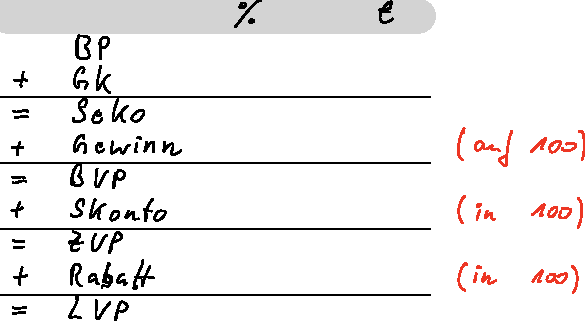
\includegraphics[width=.80\textwidth]{images/01_Verkaufskalkulation_Skizze.pdf}%
  \caption{01_Verkaufskalkulation_Skizze}%\label{fig:01_Verkaufskalkulation_Skizze}%% anpassen
\end{figure}

%\newpage
%\section{02_Umsatzerloese_Skizze}
%
%02_Umsatzerloese_Skizze (\autoref{fig:02_Umsatzerloese_Skizze}).% Referenz
%
\begin{figure}[!hb]% hier: !hb
    \centering
  \includegraphics[width=.80\textwidth]{images/02_Umsatzerloese_Skizze.pdf}%
  \caption{02_Umsatzerloese_Skizze}%\label{fig:02_Umsatzerloese_Skizze}%% anpassen
\end{figure}

%\newpage
%\section{03_Kalkulationsfaktor_Skizze}
%
%03_Kalkulationsfaktor_Skizze (\autoref{fig:03_Kalkulationsfaktor_Skizze}).% Referenz
%
\begin{figure}[!hb]% hier: !hb
    \centering
  \includegraphics[width=.80\textwidth]{images/03_Kalkulationsfaktor_Skizze.pdf}%
  \caption{03_Kalkulationsfaktor_Skizze}%\label{fig:03_Kalkulationsfaktor_Skizze}%% anpassen
\end{figure}

%\newpage
%\section{Arbeitszeitermittlung}
%
%Arbeitszeitermittlung (\autoref{fig:Arbeitszeitermittlung}).% Referenz
%
\begin{figure}[!hb]% hier: !hb
    \centering
  \includegraphics[width=.80\textwidth]{images/Arbeitszeitermittlung.pdf}%
  \caption{Arbeitszeitermittlung}%\label{fig:Arbeitszeitermittlung}%% anpassen
\end{figure}

%\newpage

%\chapter{Quellcode-files}
%% ---------------------------------
% Quellcode 'code/' in Latex speichern. 
% 'archiv/Quellcode-files.tex' 
% HTML, Python, Bash, C, C++, TeX 
% ju 17-Jul-2022 Quellcode-files.tex
% ---------------------------------
%

\section{Python_keywords}

%Python_keywords.py (\autoref{code:Python_keywords-1}).% Referenz
%
\lstset{language=Python}% HTML, Python, Bash, C, C++, TeX
\lstinputlisting[% anpassen
    caption={Quellcode in Python: Python_keywords.py}, %label={code:Python_keywords-1}
]{code/Python_keywords.py}% file

\newpage


%%%%%%%%%%%%%%%%%%%%%%%%%%%%%%%%%%%%%%%%%%%%%%%%%%

% Tabellen/

%\chapter{PDFs}
%% ju 15-5-2022 input-PDFs.txt 

\chapter{Rechenbeispiele}% book, print anpassen

% -------
\section{Umsatzerlöse}\label{sec:01-Umsatzerloese}\index{01-Umsatzerloese}
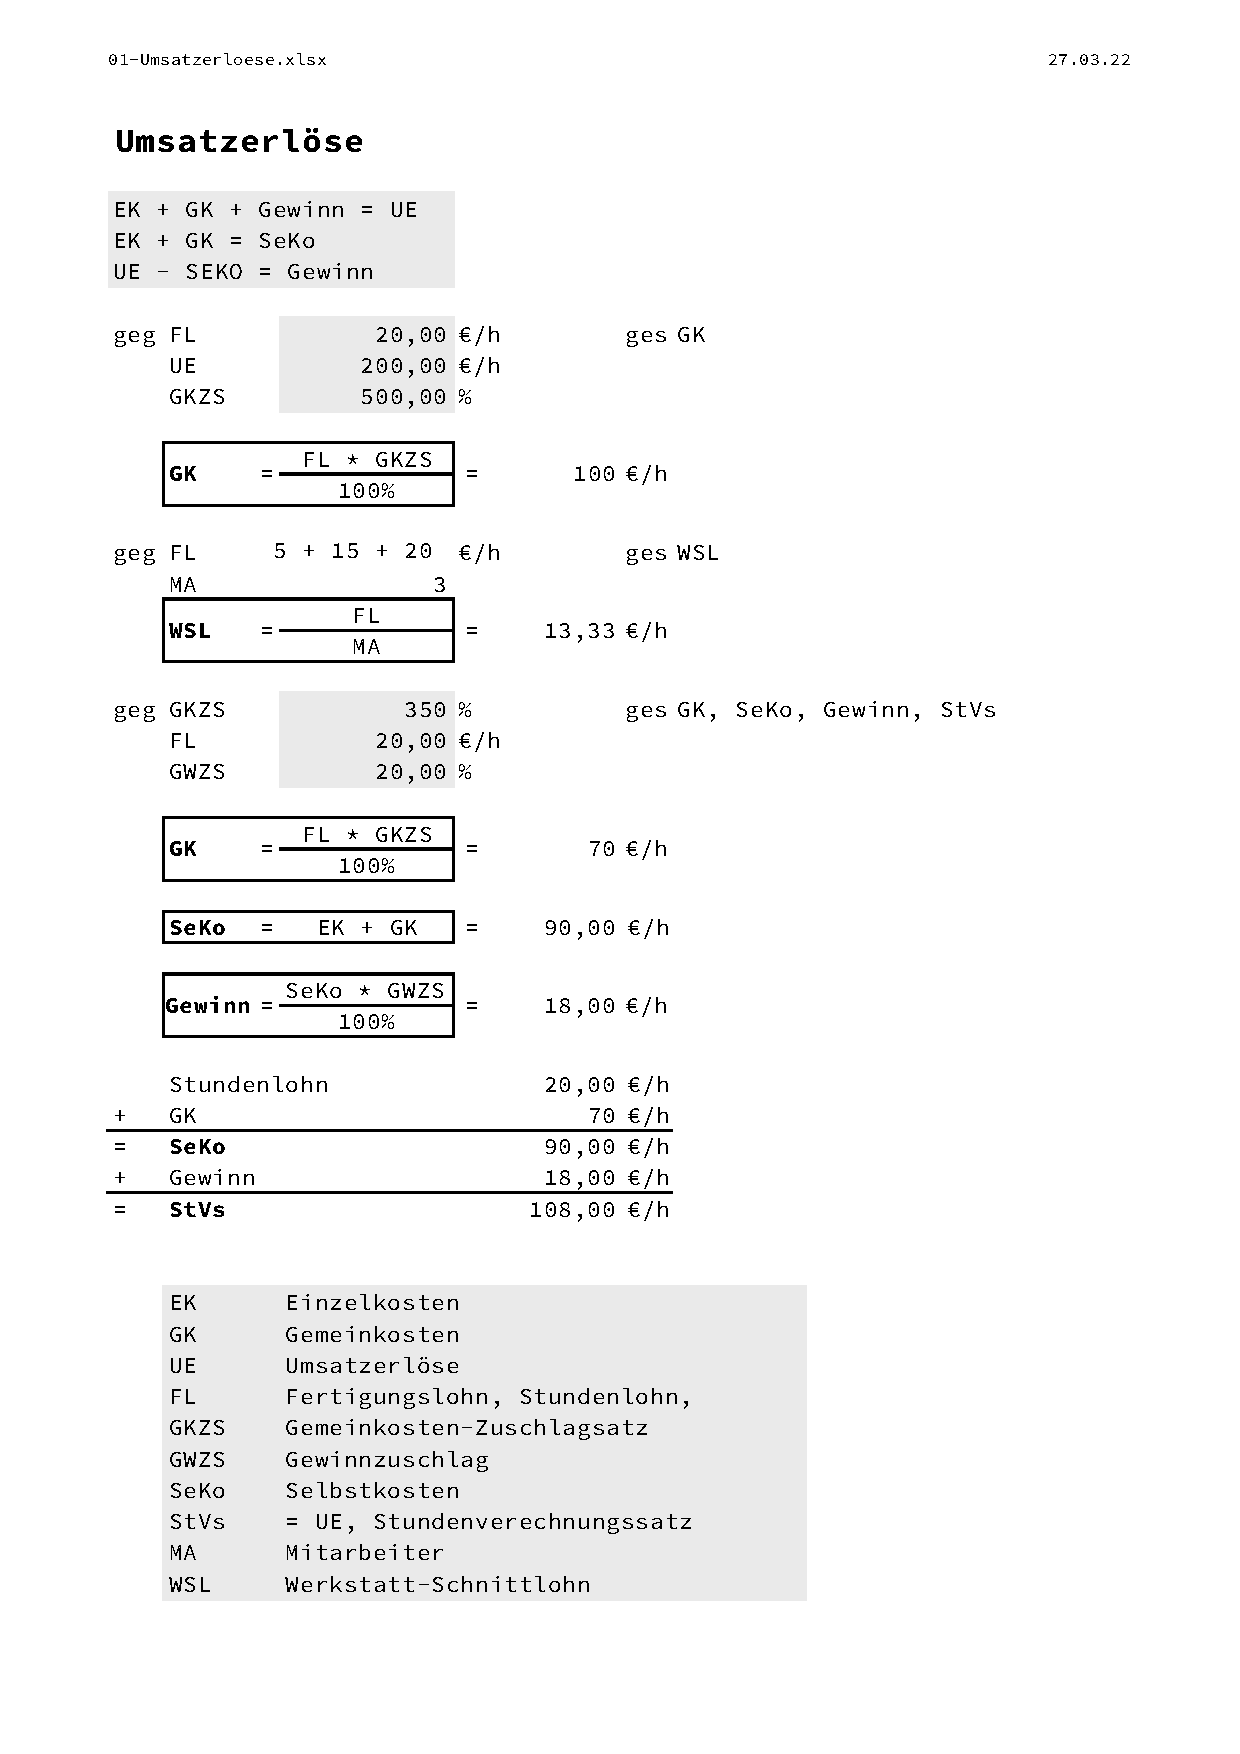
\includepdf[pages=-]{Tabellen/PDF/01-Umsatzerloese.pdf}

% -------
\section{AT-Steuer}\label{sec:02-AT-Steuer}\index{02-AT-Steuer}
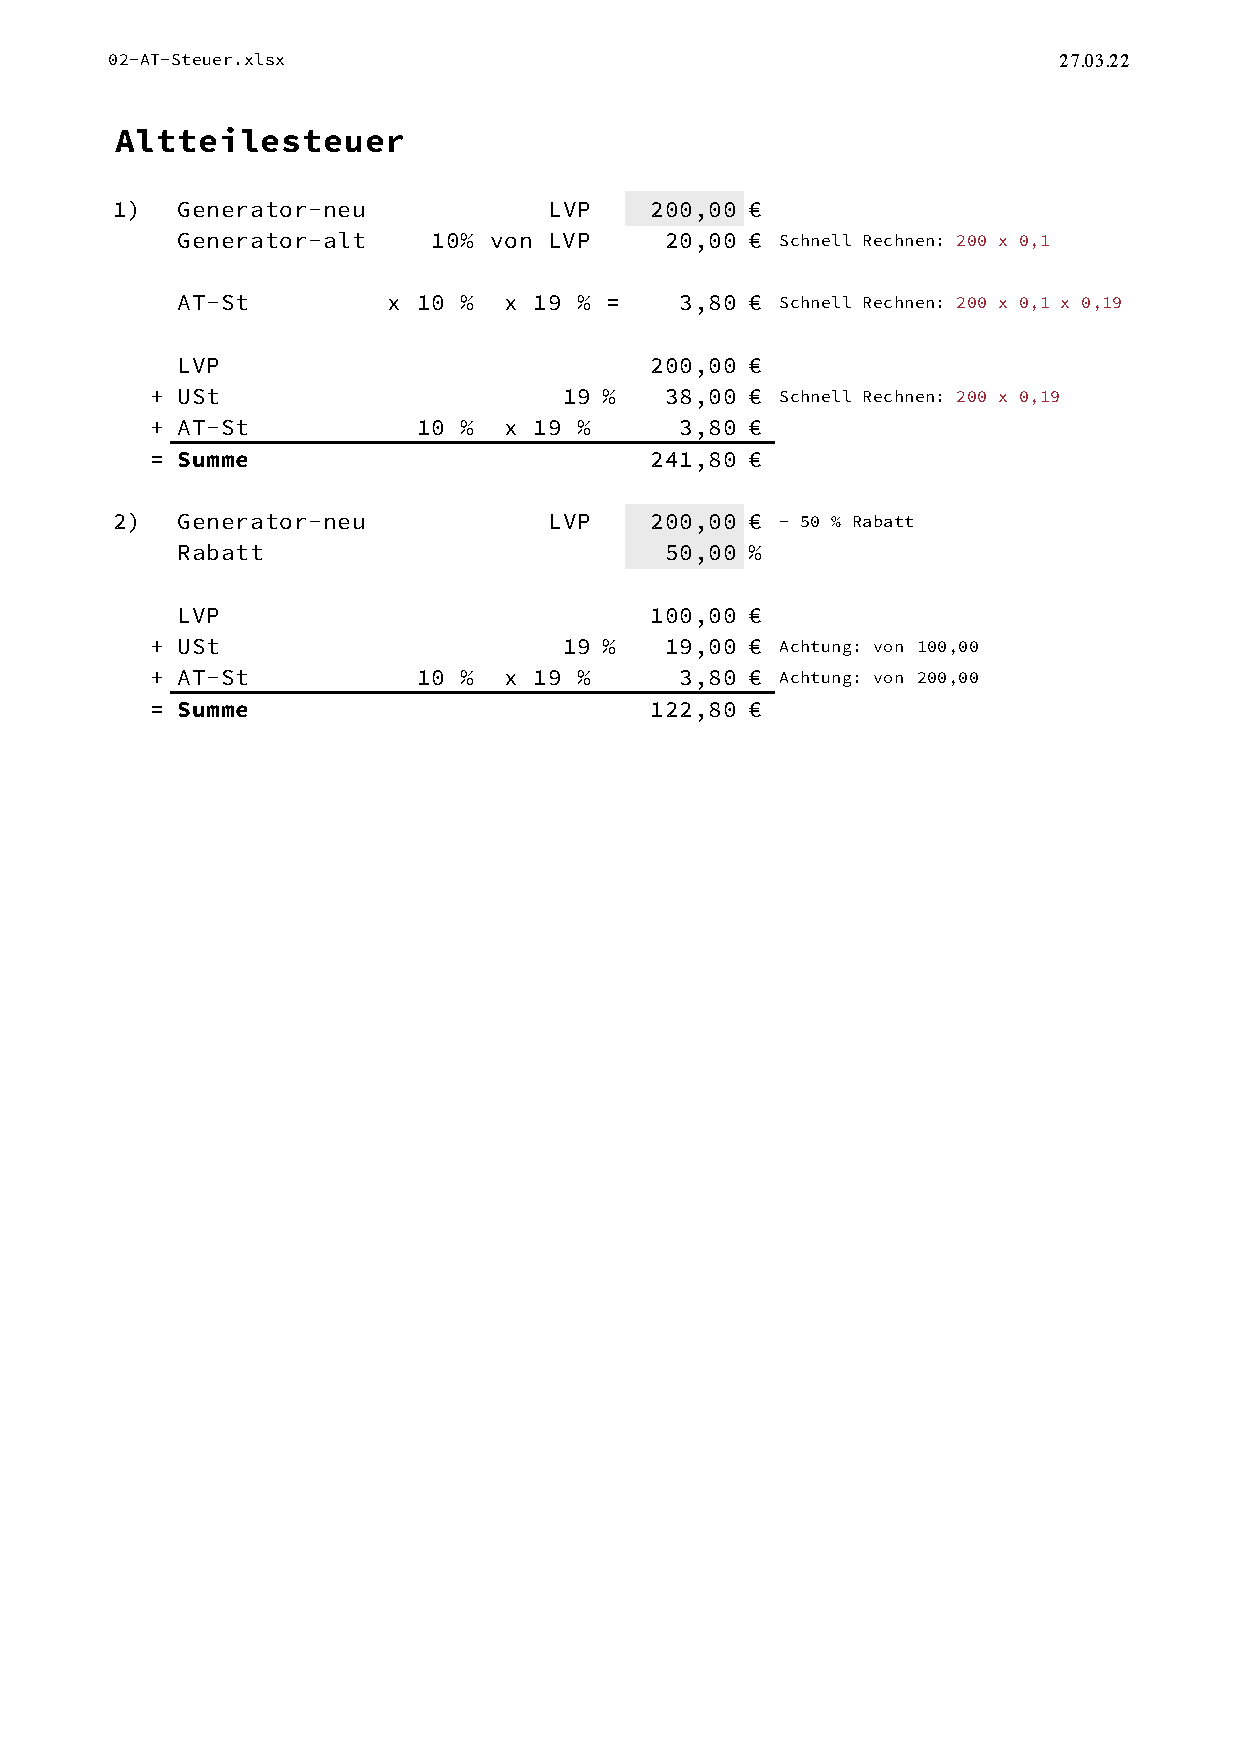
\includepdf[pages=-]{Tabellen/PDF/02-AT-Steuer.pdf}

% -------
\section{Ersatzteilpreiskalkulation}\label{sec:03-Ersatzteilpreiskalkulation}\index{03-Ersatzteilpreiskalkulation}
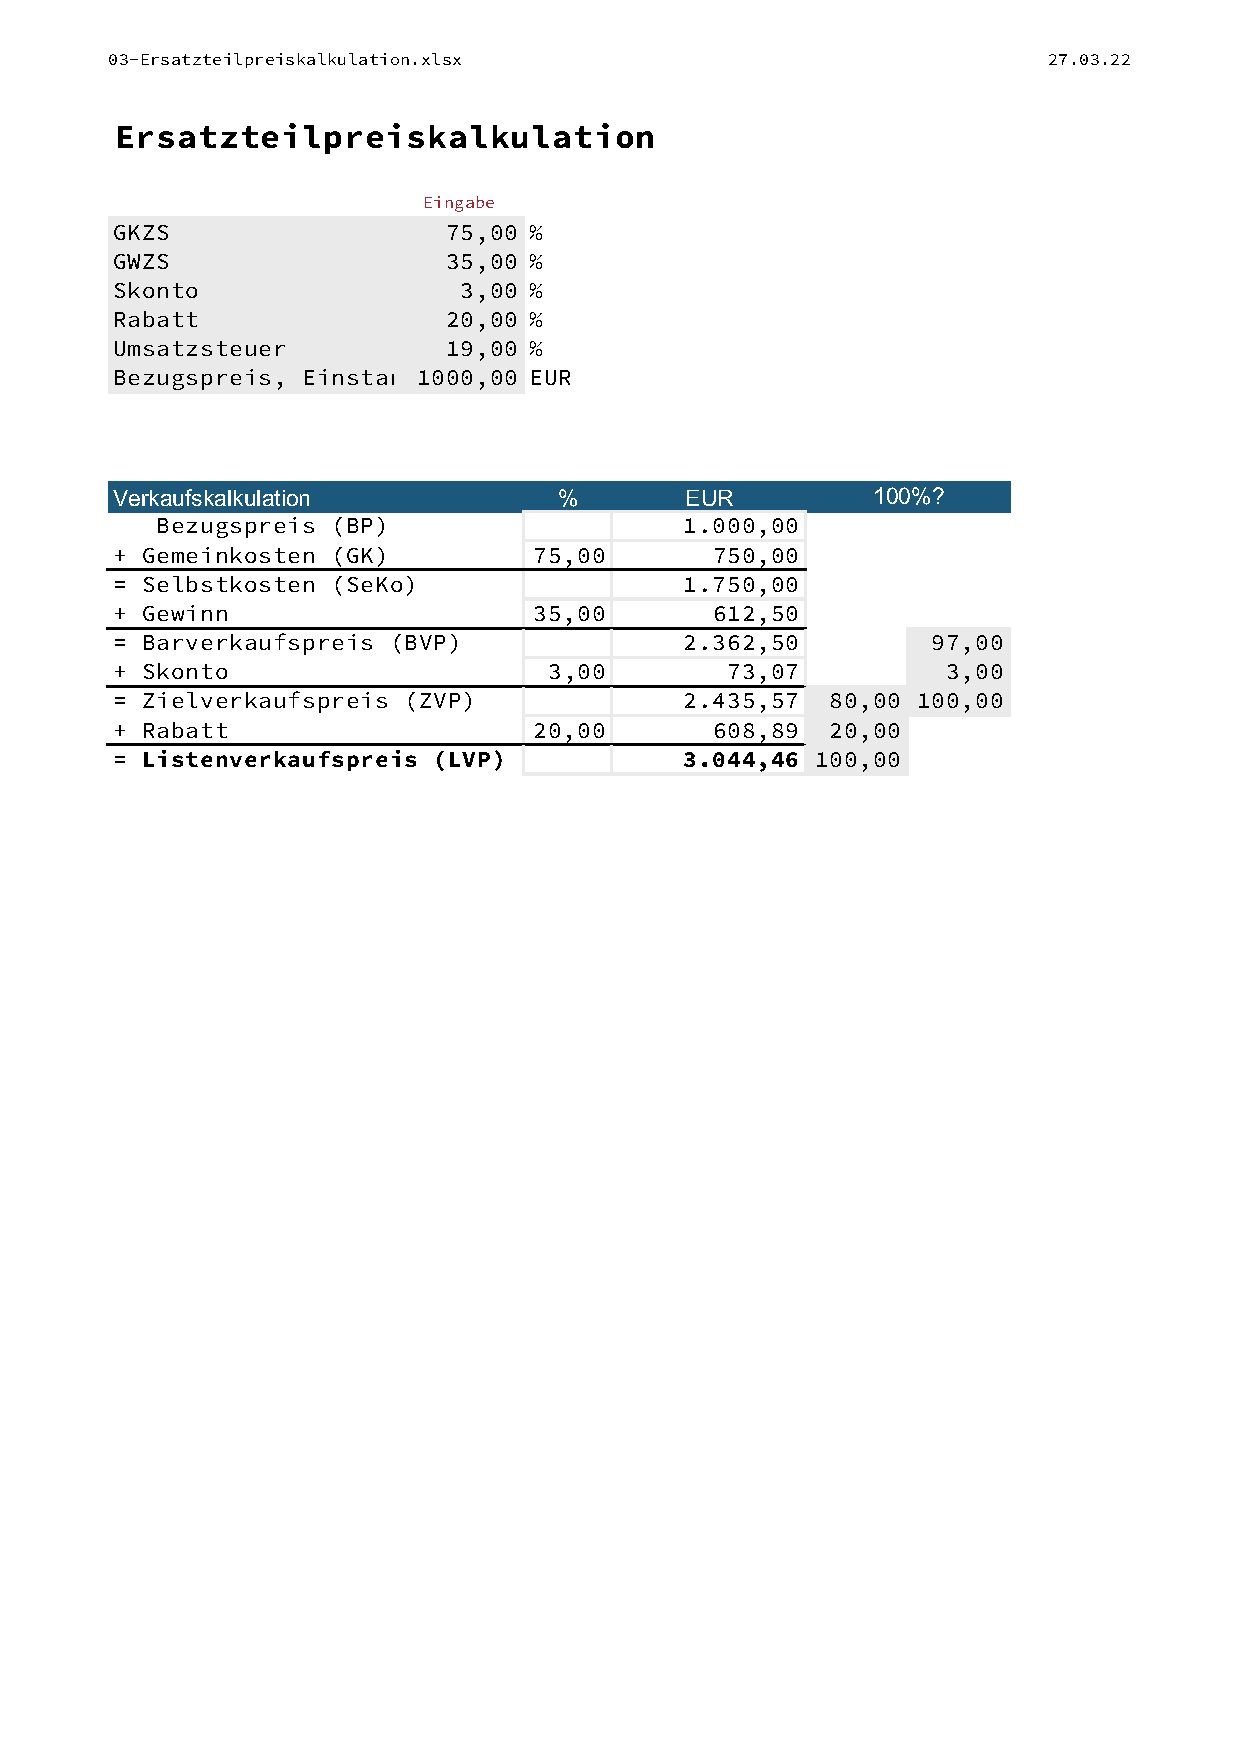
\includepdf[pages=-]{Tabellen/PDF/03-Ersatzteilpreiskalkulation.pdf}




\chapter{Übungsaufgaben}

% -------
\section{U01 - Ersatzteilpreiskalkulation - KI - HSP - KF}\label{sec:U01-Ersatzteilpreiskalkulation-KI-HSP-KF}\index{U01-Ersatzteilpreiskalkulation-KI-HSP-KF}
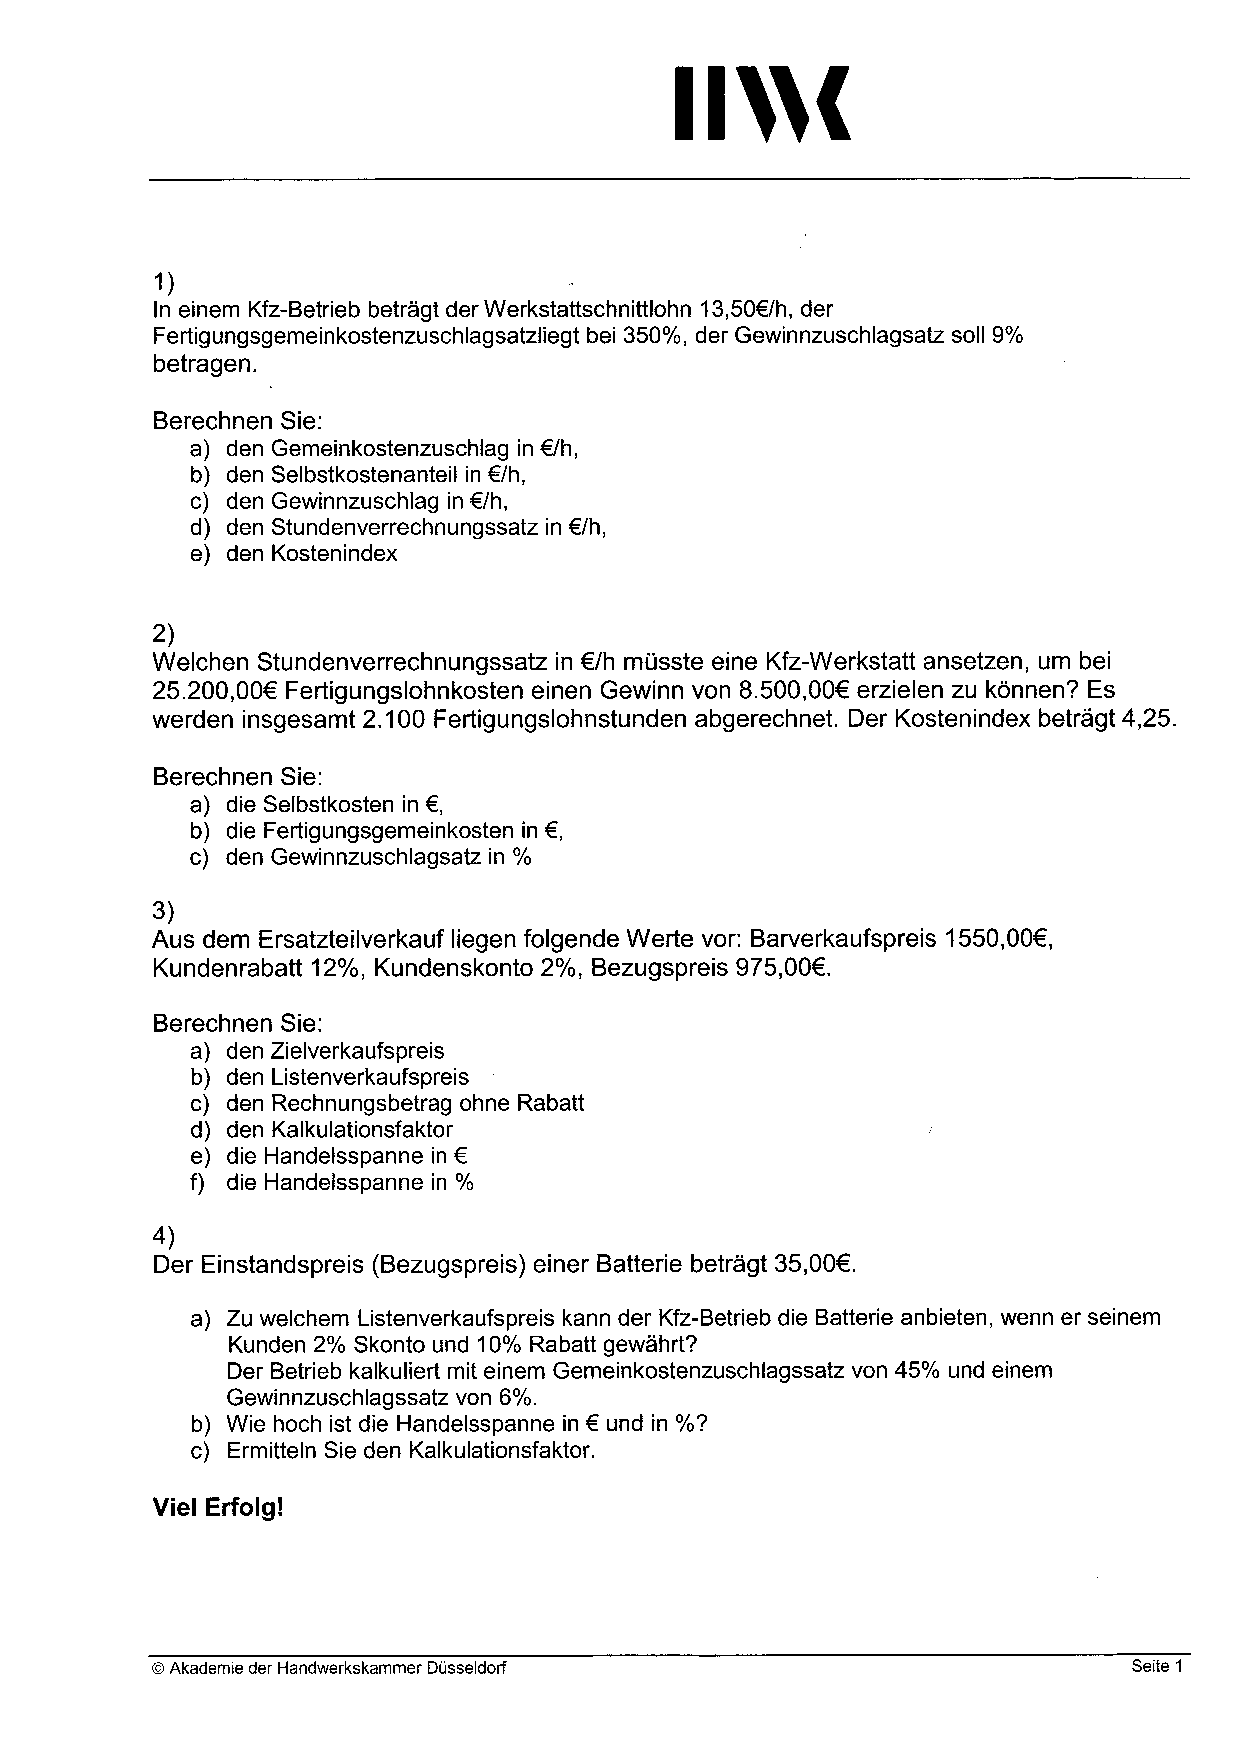
\includepdf[pages=-]{Tabellen/PDF/U01-Ersatzteilpreiskalkulation-KI-HSP-KF.pdf}
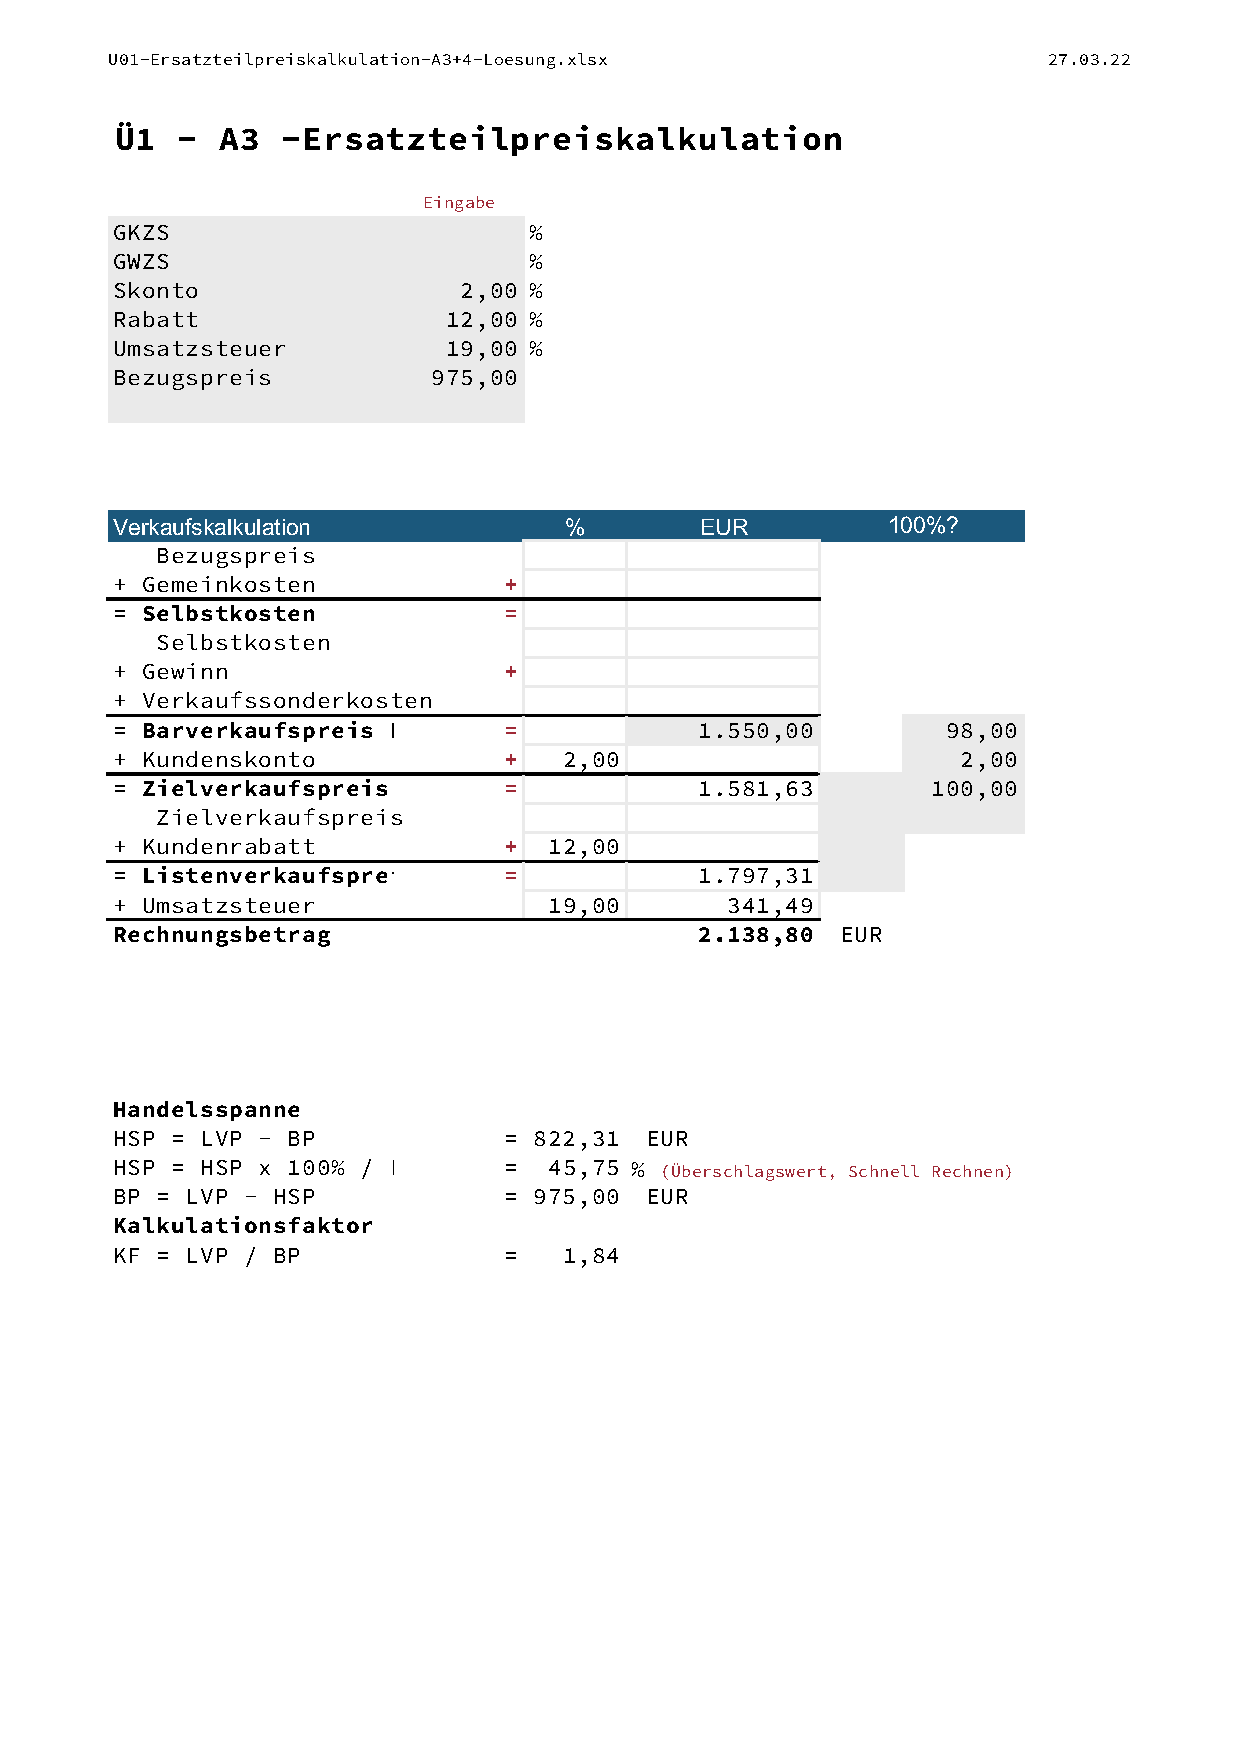
\includepdf[pages=-]{Tabellen/PDF/U01-Ersatzteilpreiskalkulation-A3+4-Loesung.pdf}

% -------
\section{U02 - StVs - WI - KI - Kostenvoranschlag}\label{sec:U02-StVs-WI-KI-Kostenvoranschlag}\index{U02-StVs-WI-KI-Kostenvoranschlag}
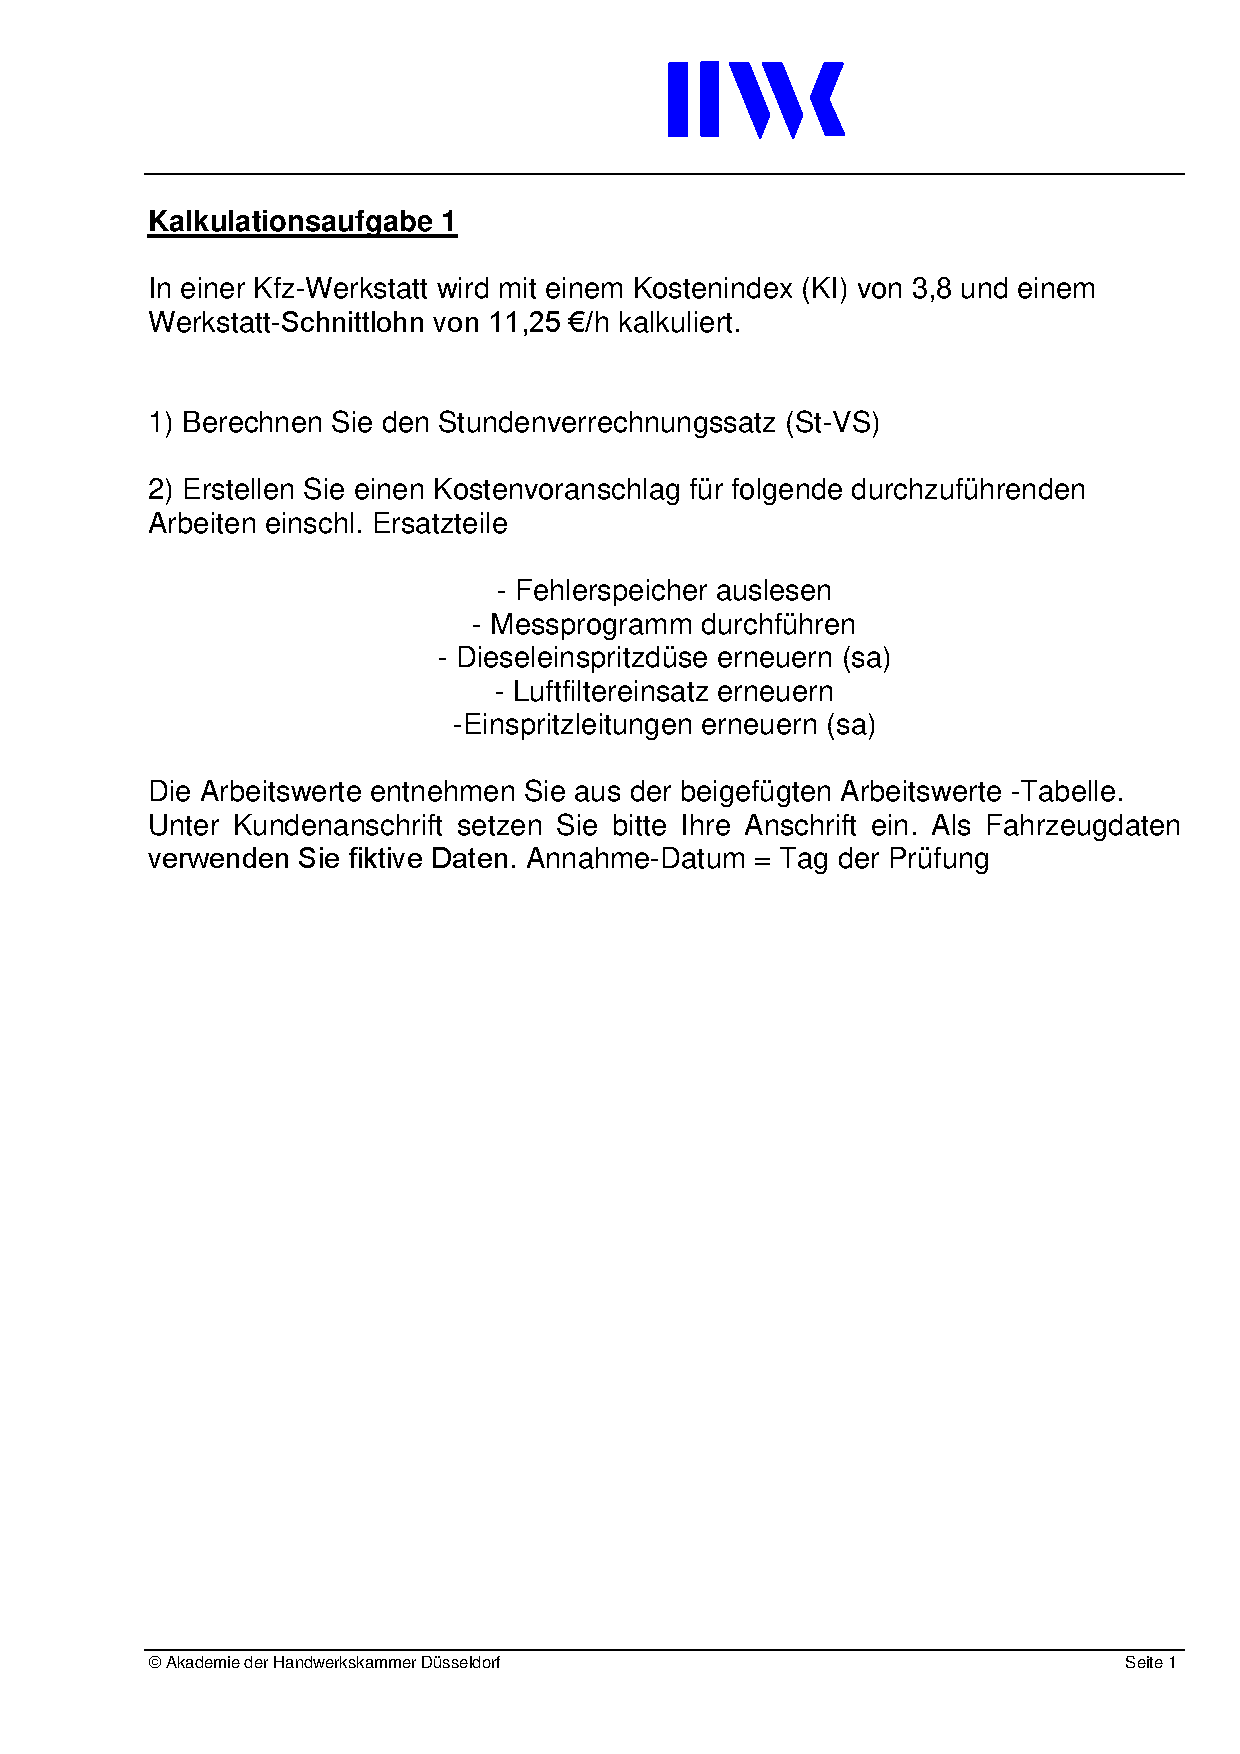
\includepdf[pages=-]{Tabellen/PDF/U02-StVs-WI-KI-Kostenvoranschlag.pdf}
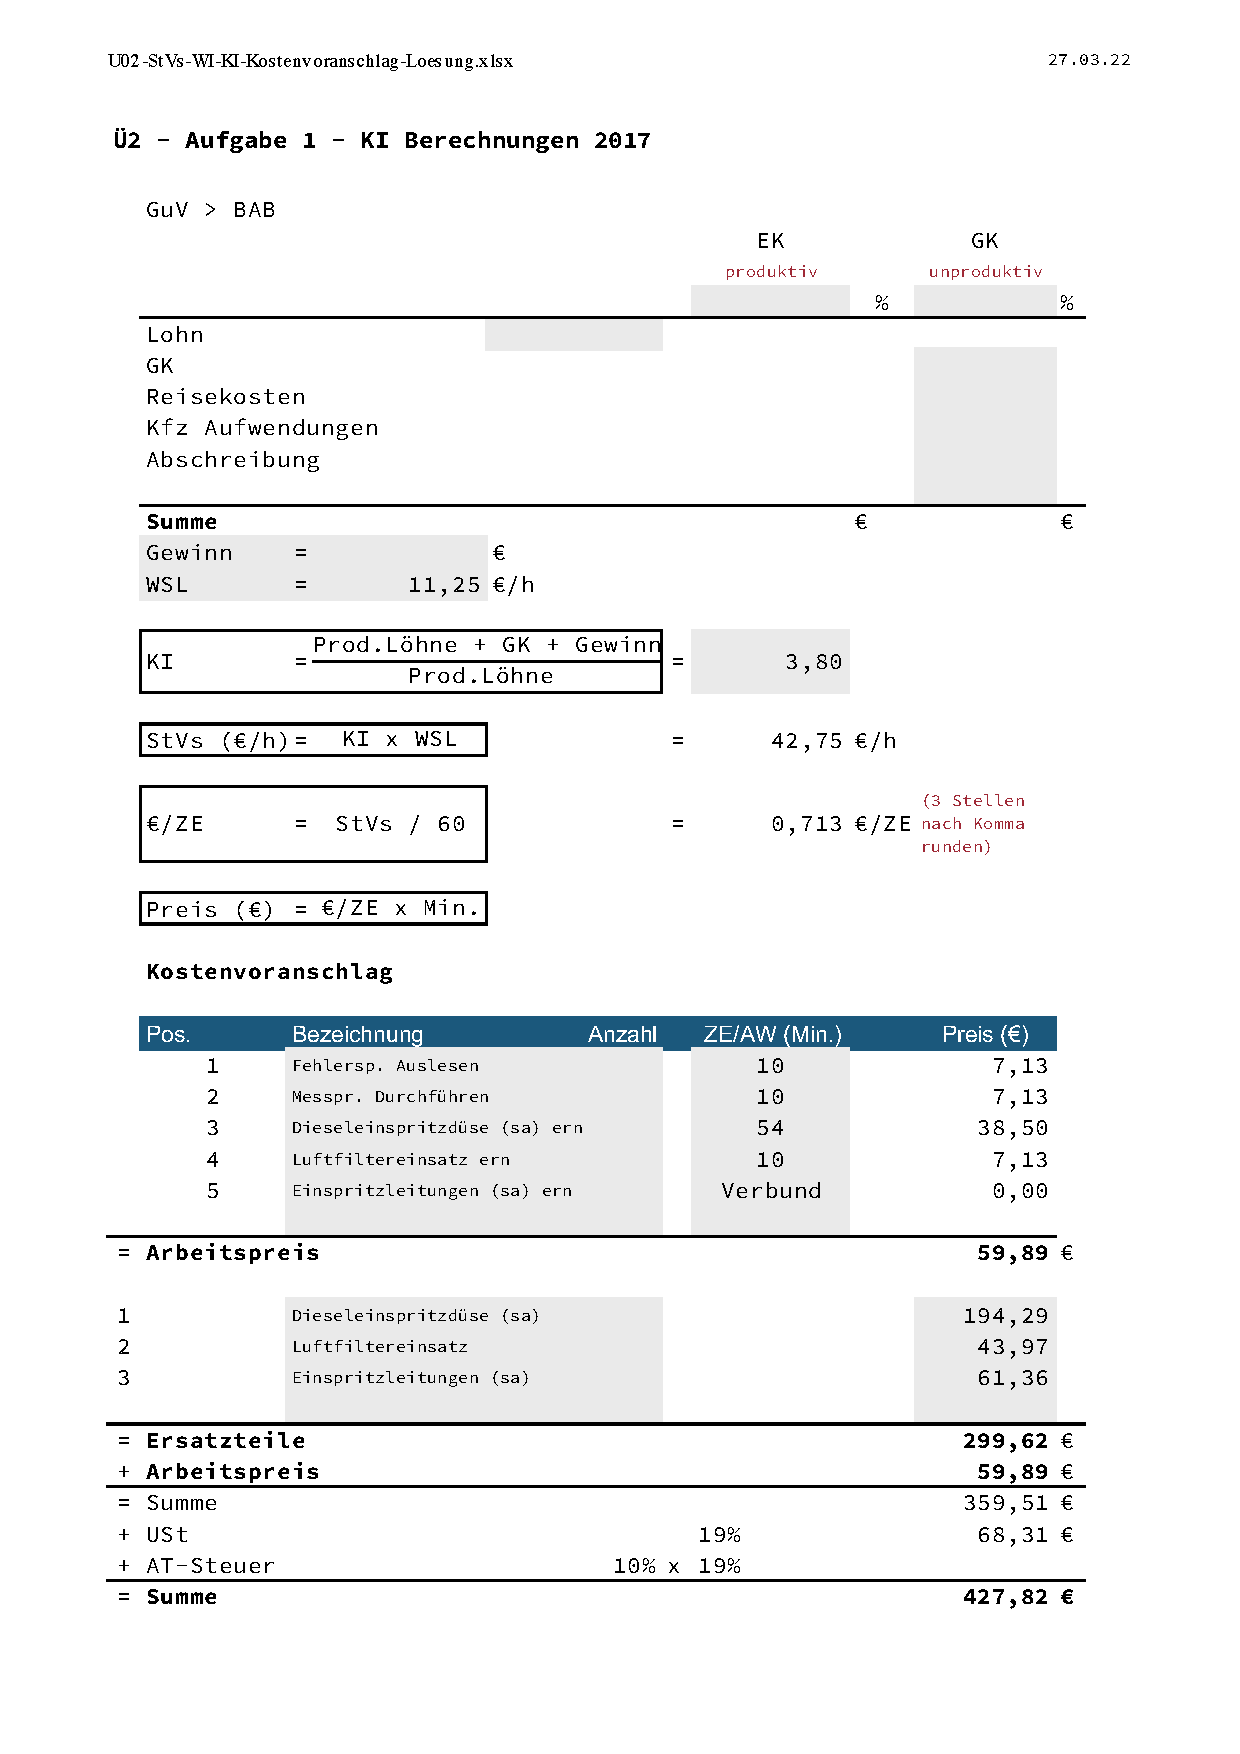
\includepdf[pages=-]{Tabellen/PDF/U02-StVs-WI-KI-Kostenvoranschlag-Loesung.pdf}

% -------
\section{U03 - Kundenrechnung - Kostenvoranschlag - AW-Vs - UR - WI}\label{sec:U03-Kundenrechnung-Kostenvoranschlag-AW-Vs-UR-WI}\index{U03-Kundenrechnung-Kostenvoranschlag-AW-Vs-UR-WI}
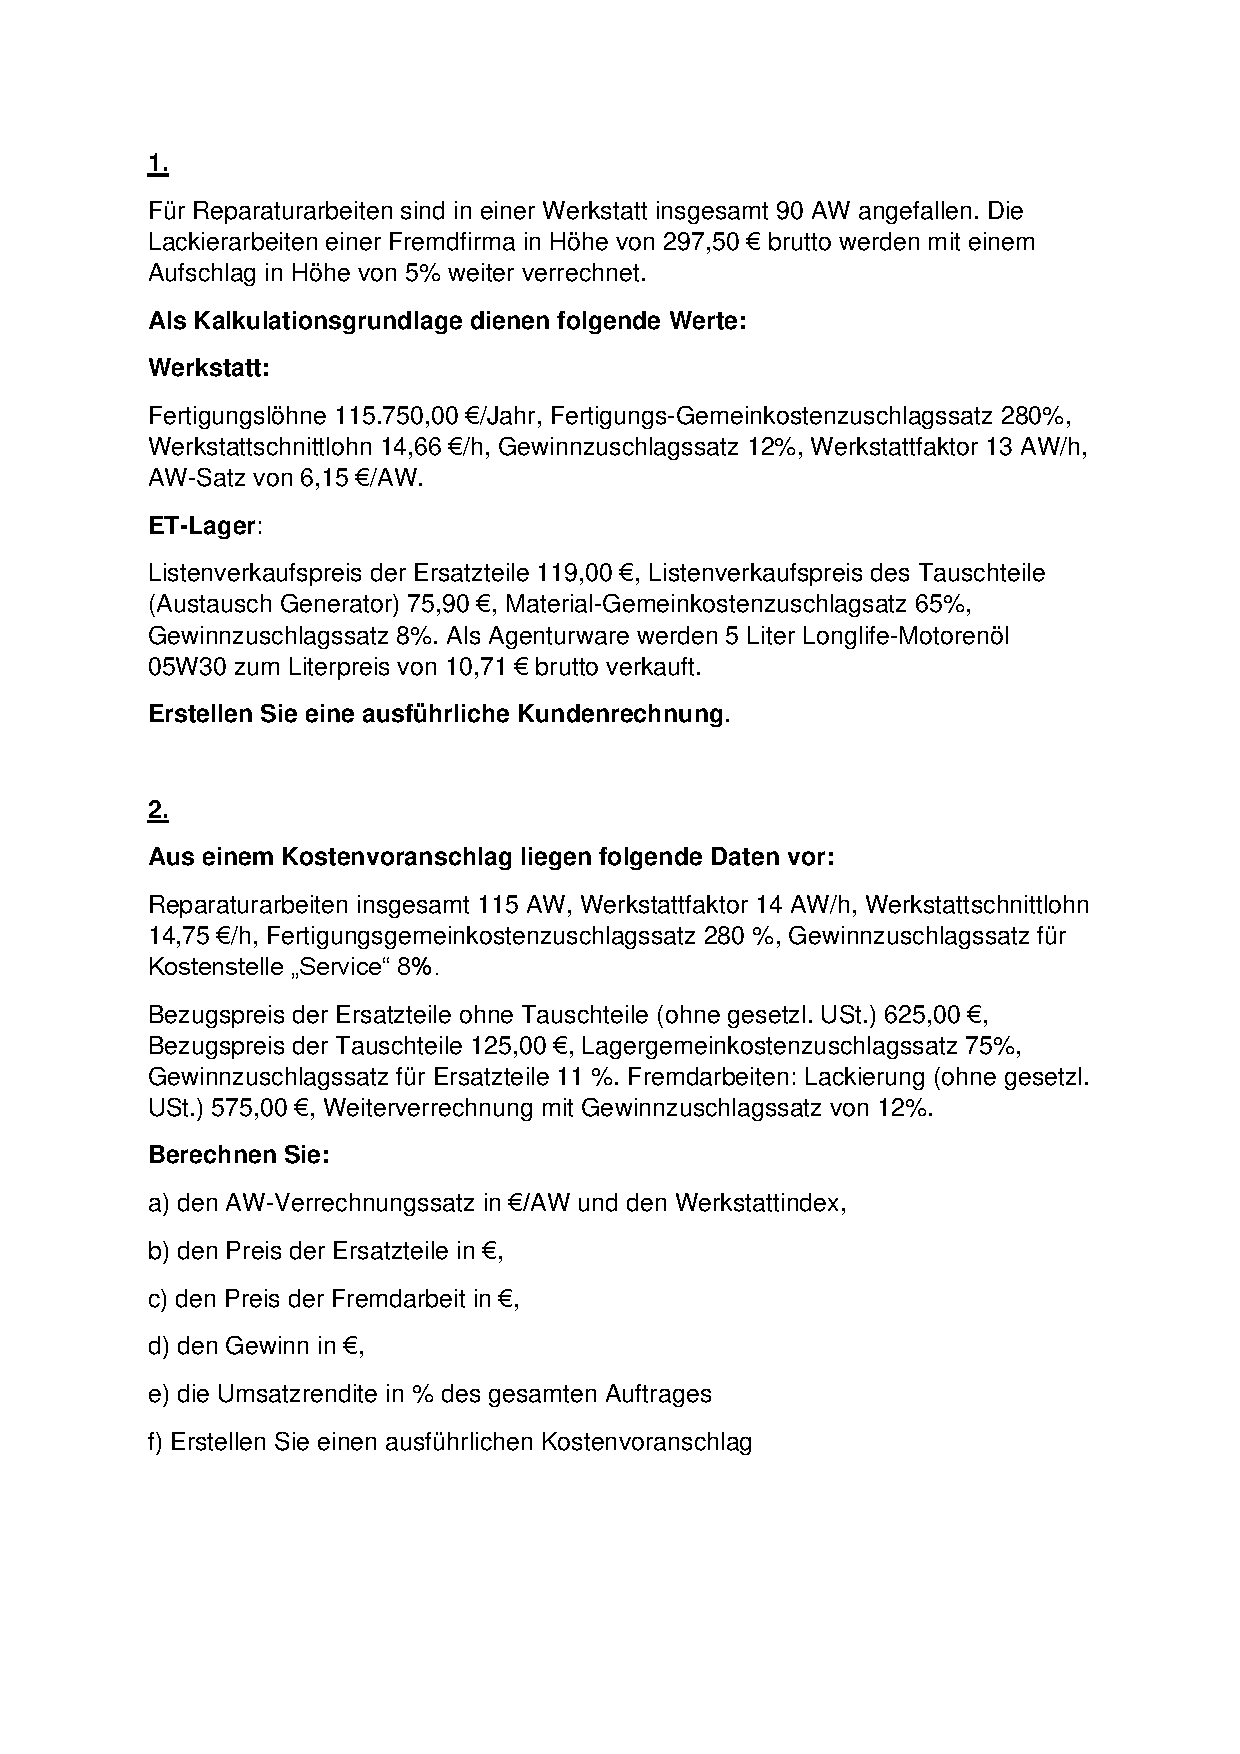
\includepdf[pages=-]{Tabellen/PDF/U03-Kundenrechnung-Kostenvoranschlag-AW-Vs-UR-WI.pdf}}
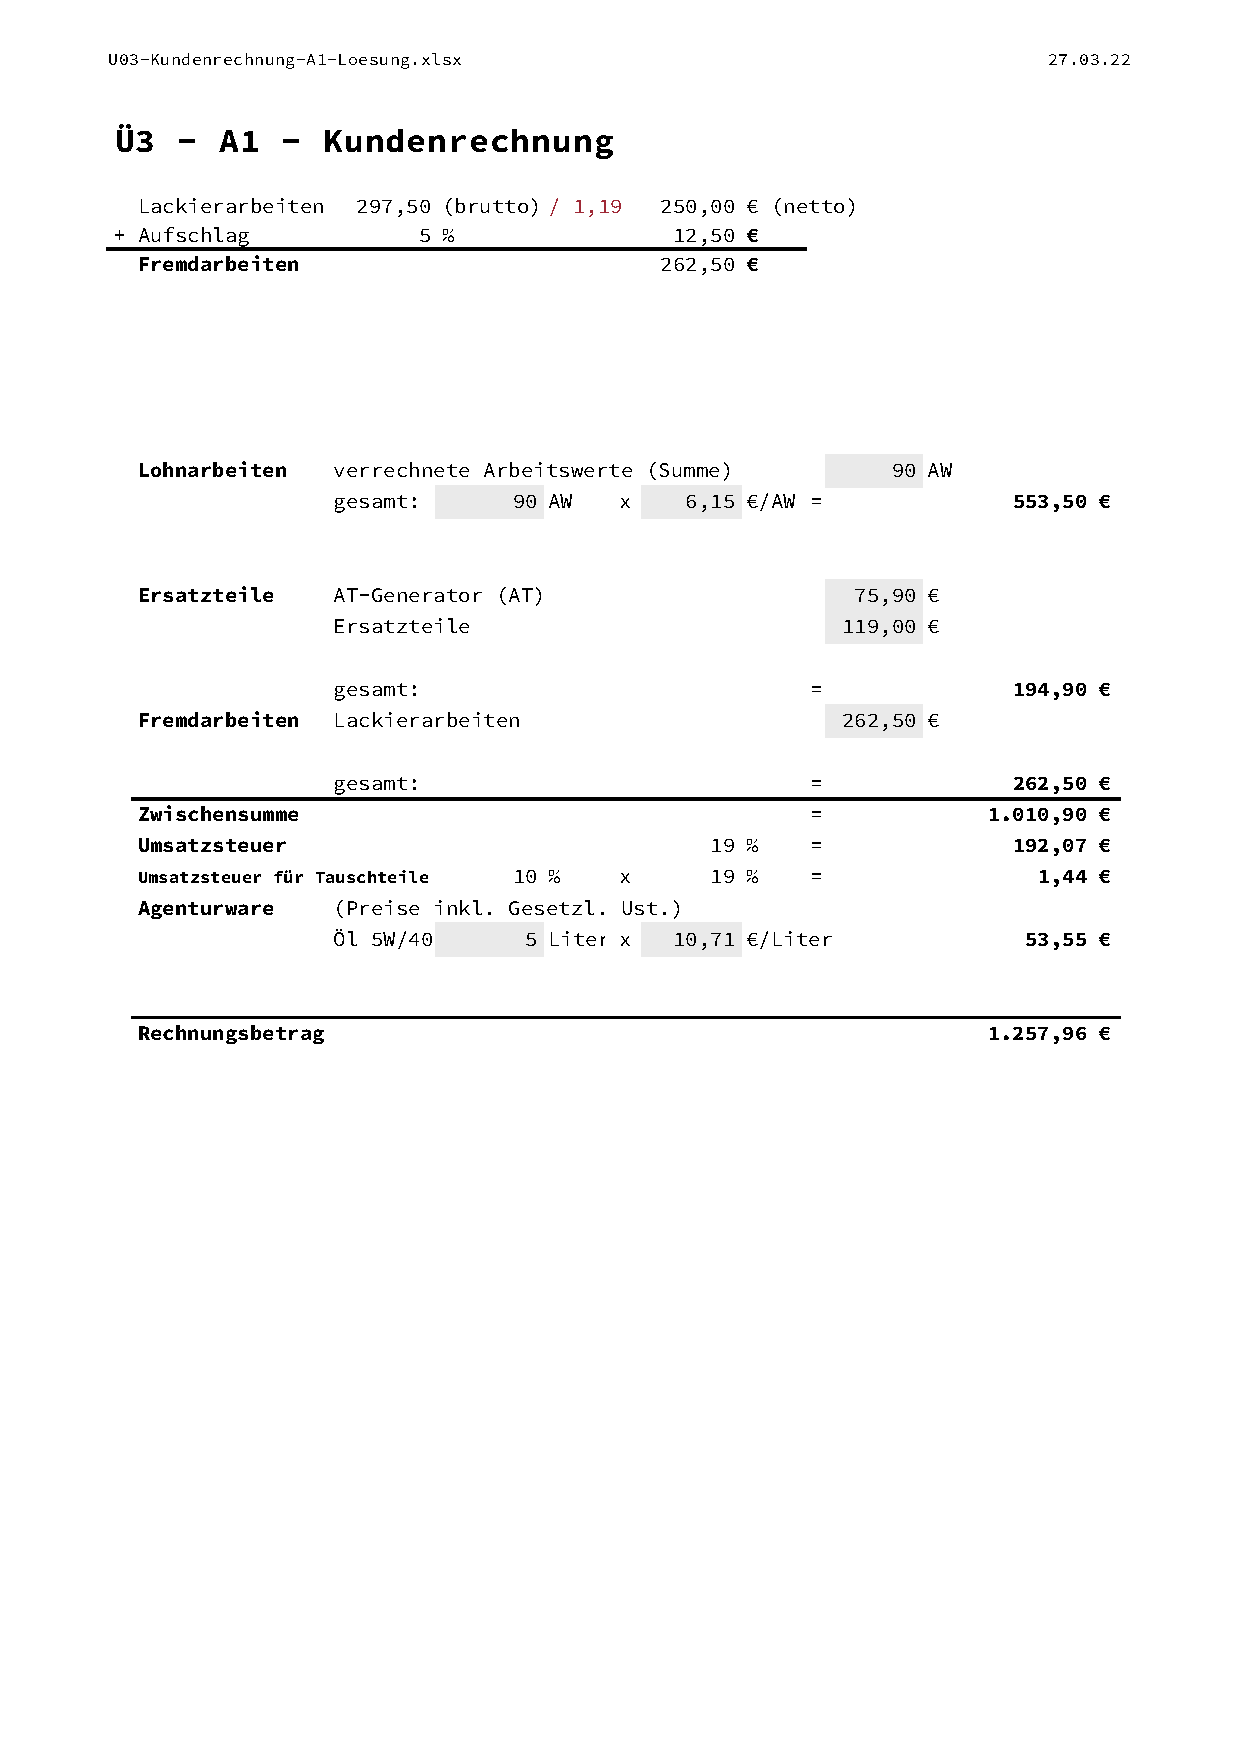
\includepdf[pages=-]{Tabellen/PDF/U03-Kundenrechnung-A1-Loesung.pdf}

% -------
\section{U04 - Werkstattabrechnung - Arbeitszeit - A1 - 4 von 10}\label{sec:U04-Werkstattabrechnung-Arbeitszeit_1-4_von10}\index{U04-Werkstattabrechnung-Arbeitszeit_1-4_von10}
\includepdf[pages=-]{Tabellen/PDF/U04-Werkstattabrechnung-Arbeitszeit_1-4_von10.pdf}

% -------
\section{U05 - Gesamtarbeitszeit - StVs - AW-Vs - Flh}\label{sec:U05-Gesamtarbeitszeit-StVs-AW-Vs-Flh}\index{U05-Gesamtarbeitszeit-StVs-AW-Vs-Flh}
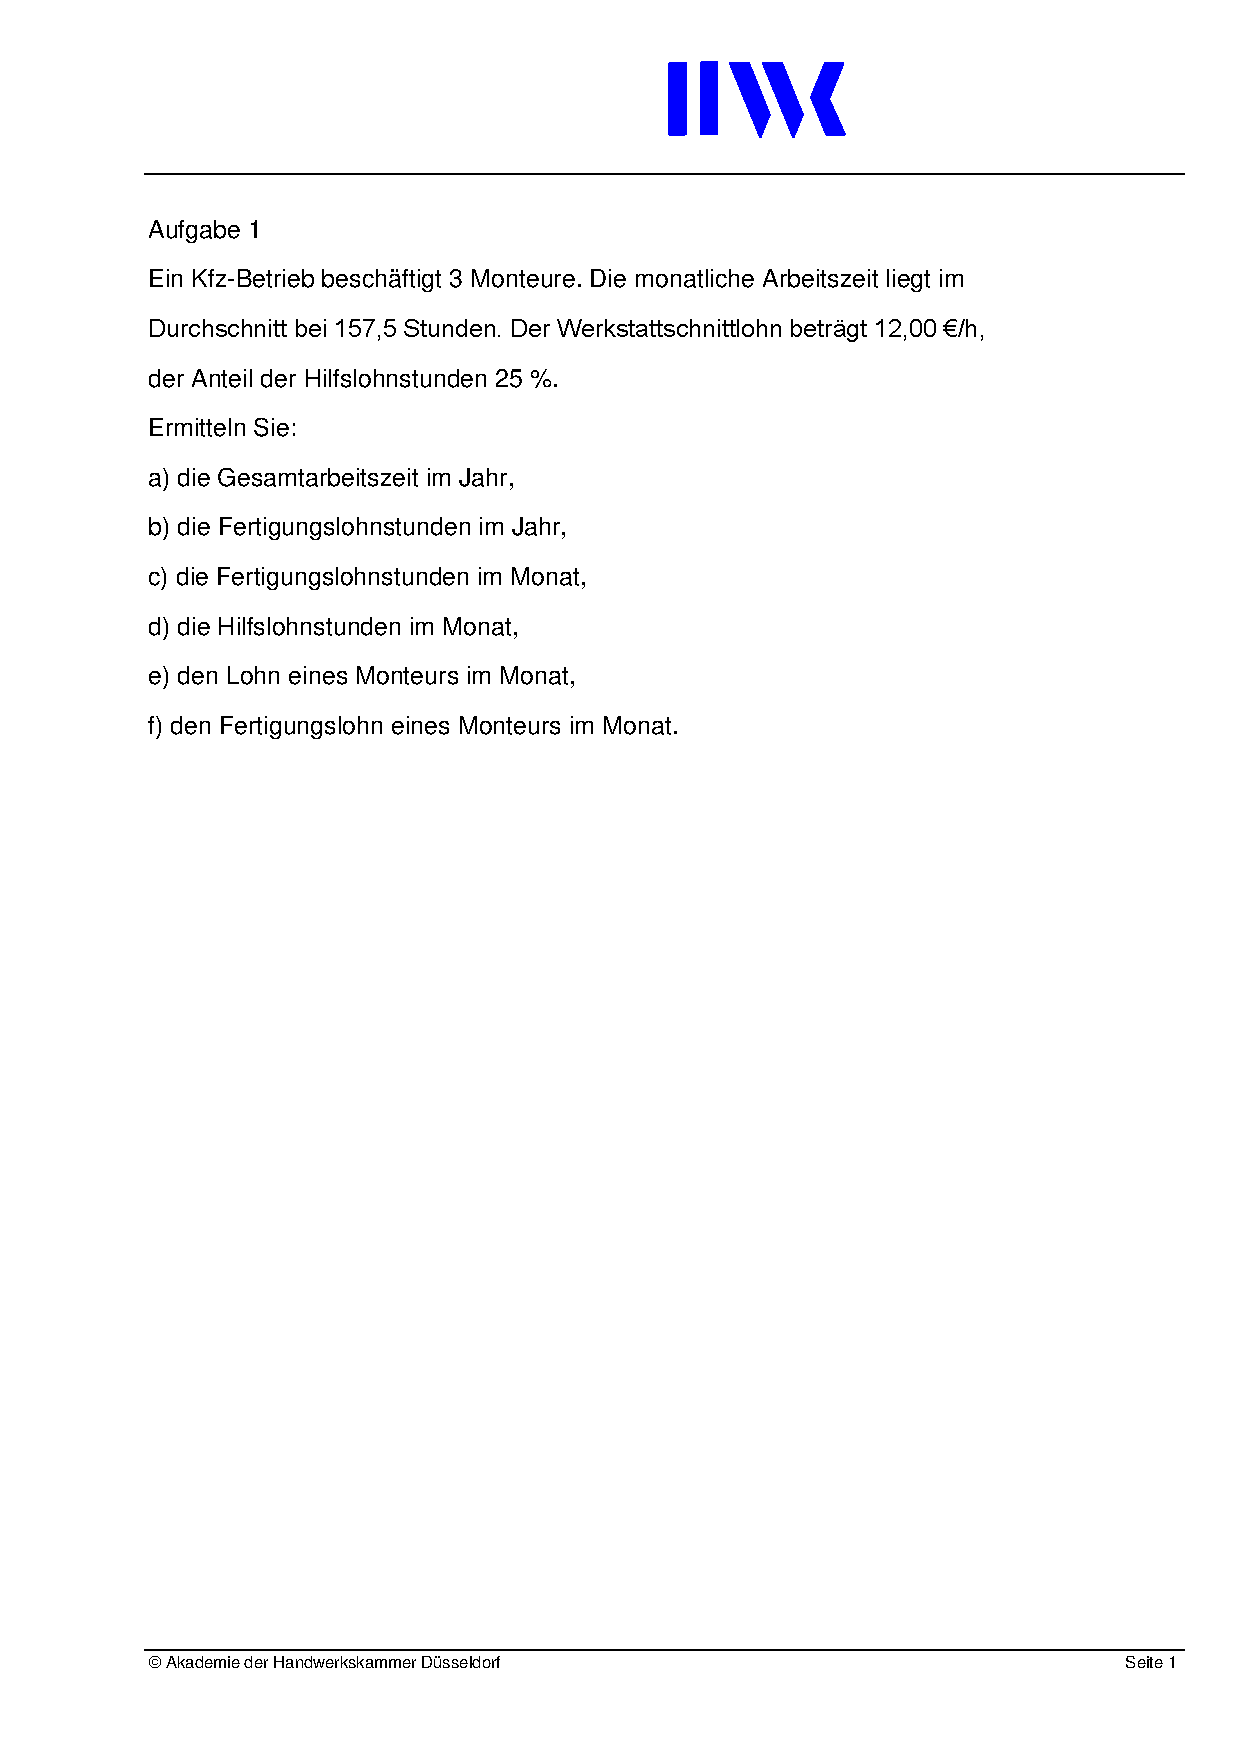
\includepdf[pages=-]{Tabellen/PDF/U05-Gesamtarbeitszeit-StVs-AW-Vs-Flh.pdf}

% -------
\section{U06 - Situationsaufgabe - Fritz}\label{sec:U06-Situationsaufgabe-Fritz-Loesung}\index{U06-Situationsaufgabe-Fritz-Loesung}
%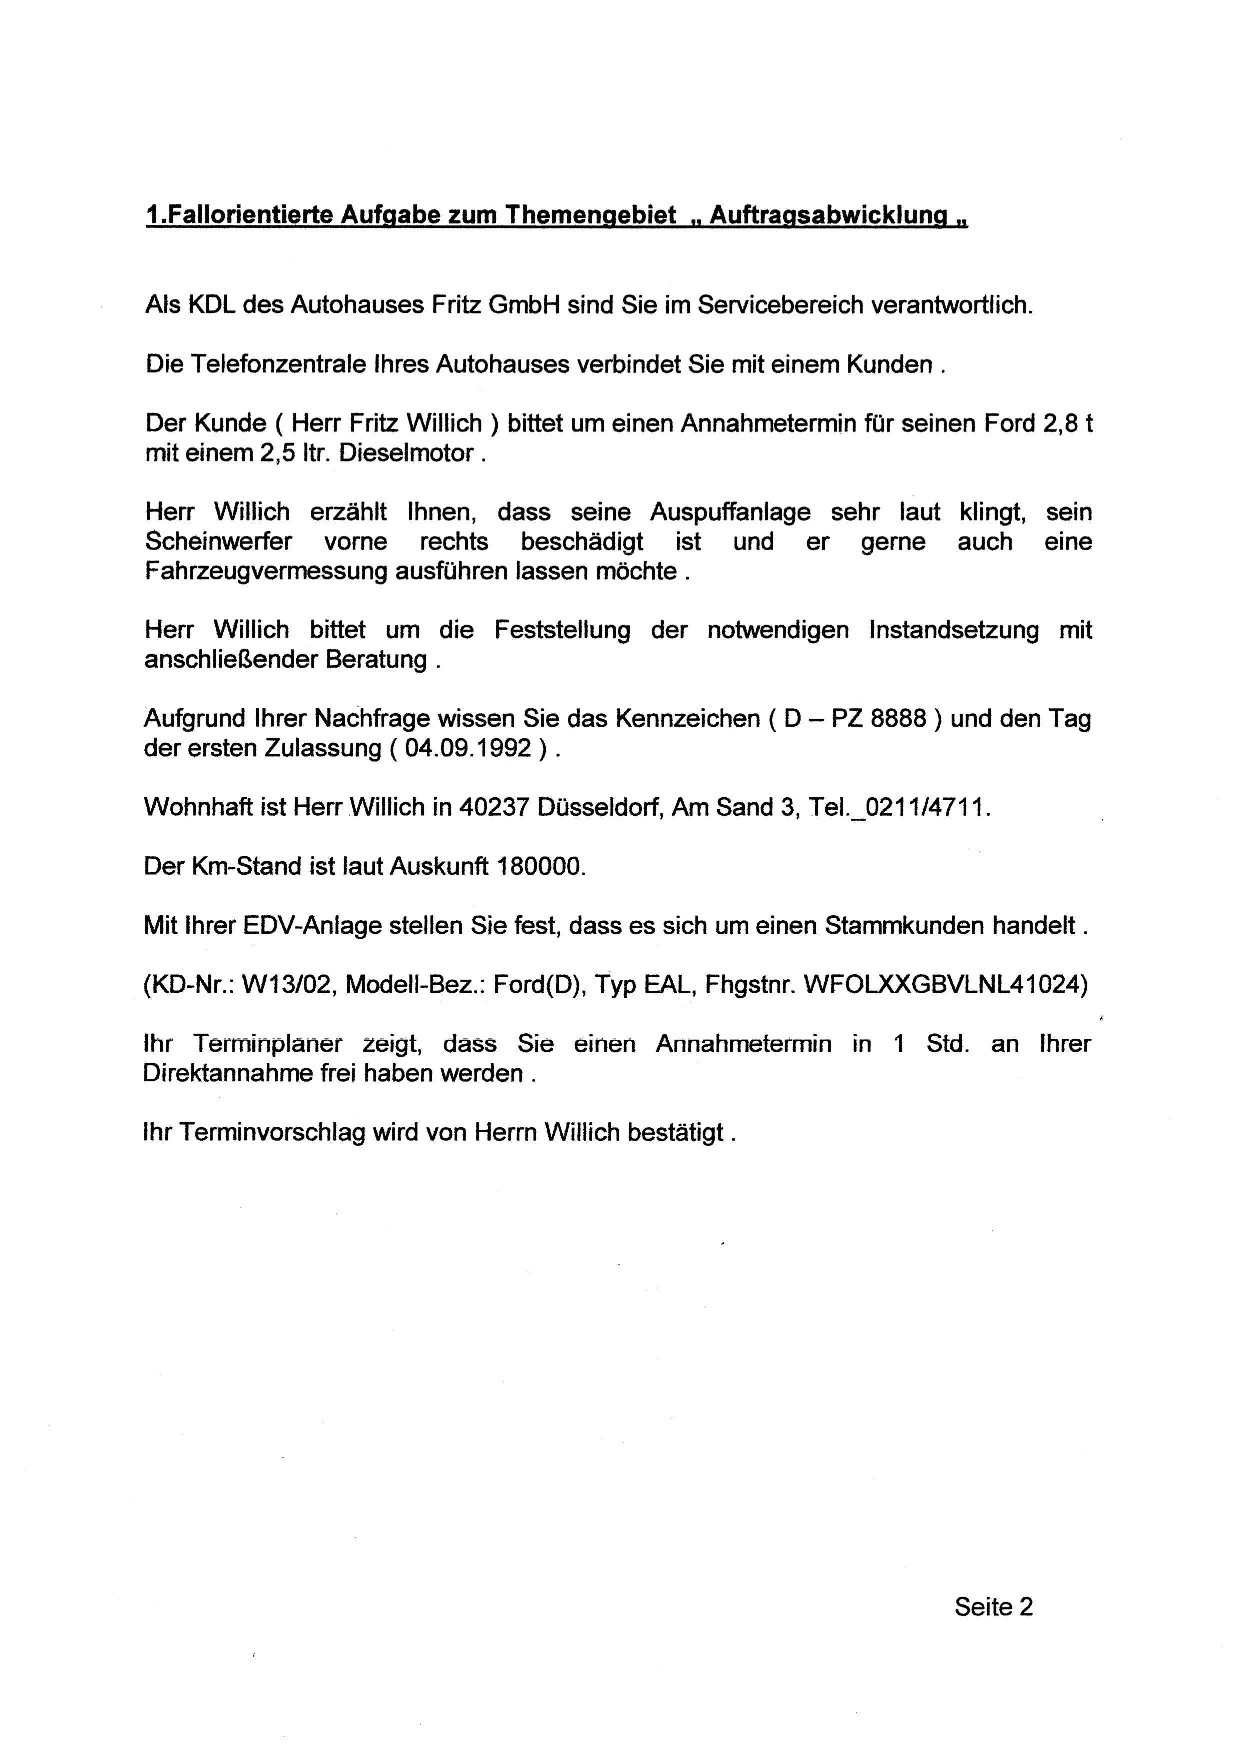
\includepdf[pages=-]{Tabellen/PDF/U06-Situationsaufgabe-Fritz-Loesung.pdf}
%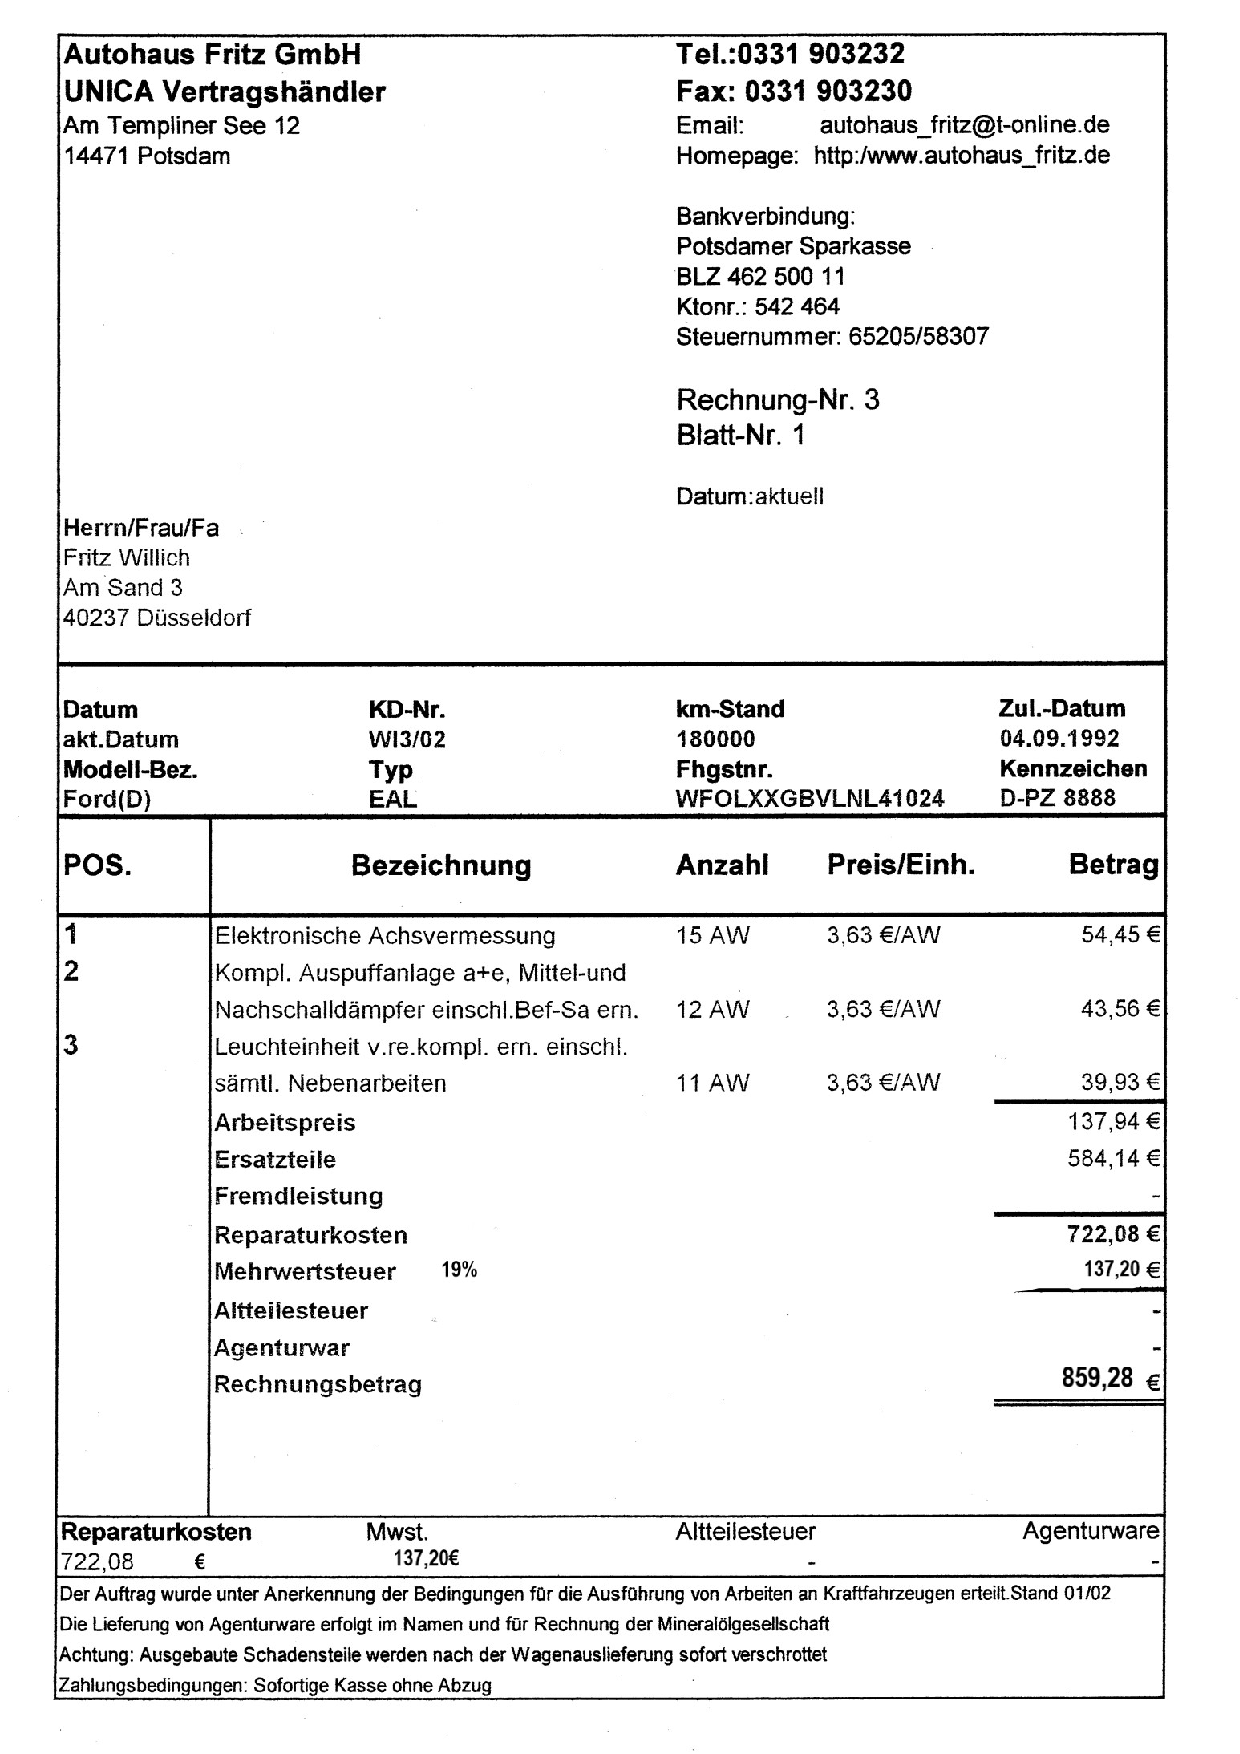
\includepdf[pages=-]{Tabellen/PDF/U06-Situationsaufgabe-Fritz-Rechnung.pdf}
%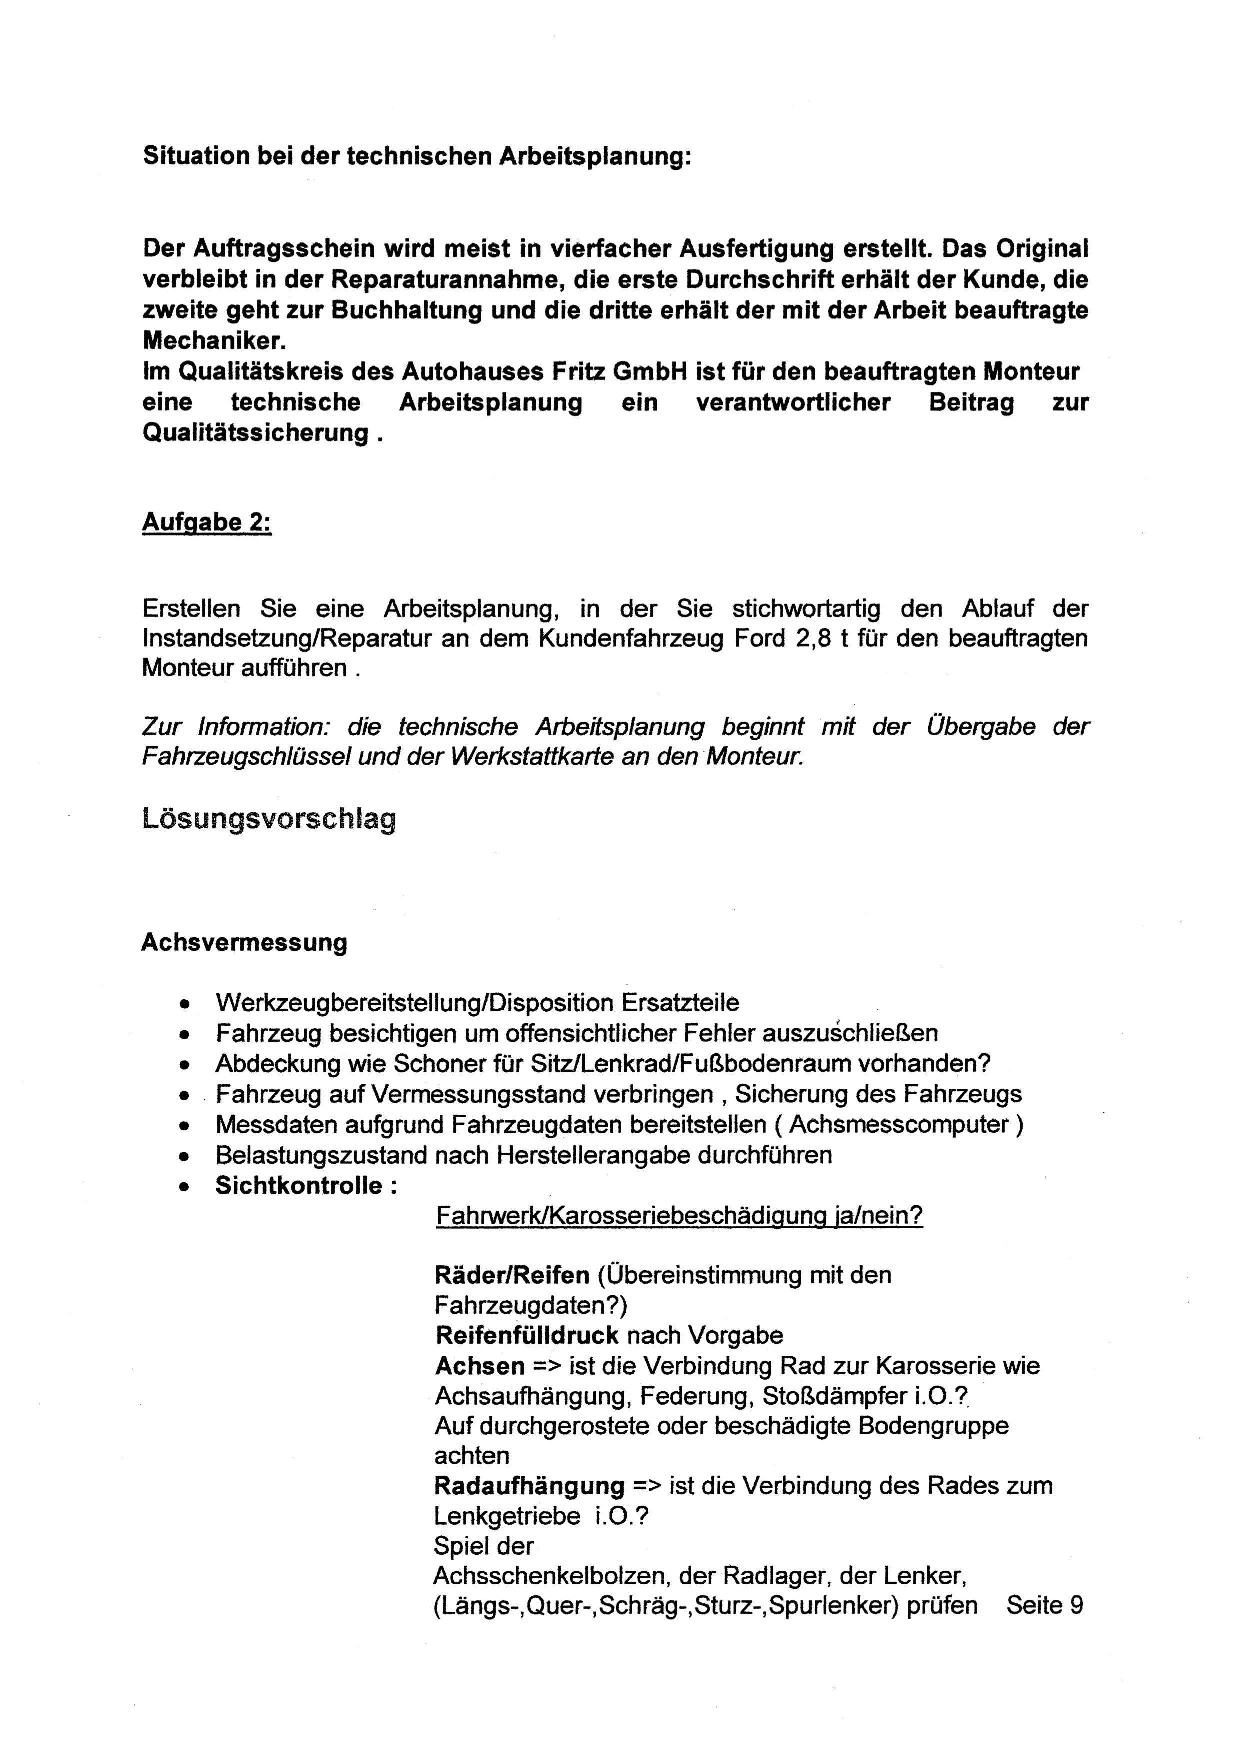
\includepdf[pages=-]{Tabellen/PDF/U06-Situationsaufgabe-Fritz-Arbeitsplanung.pdf}


% -------
\section{U07 - Aufgabe - KV1 - Stauscheibenpoti - AT}\label{sec:U07-Aufgabe-KV1-Stauscheibenpoti-AT}\index{U07-Aufgabe-KV1-Stauscheibenpoti-AT}
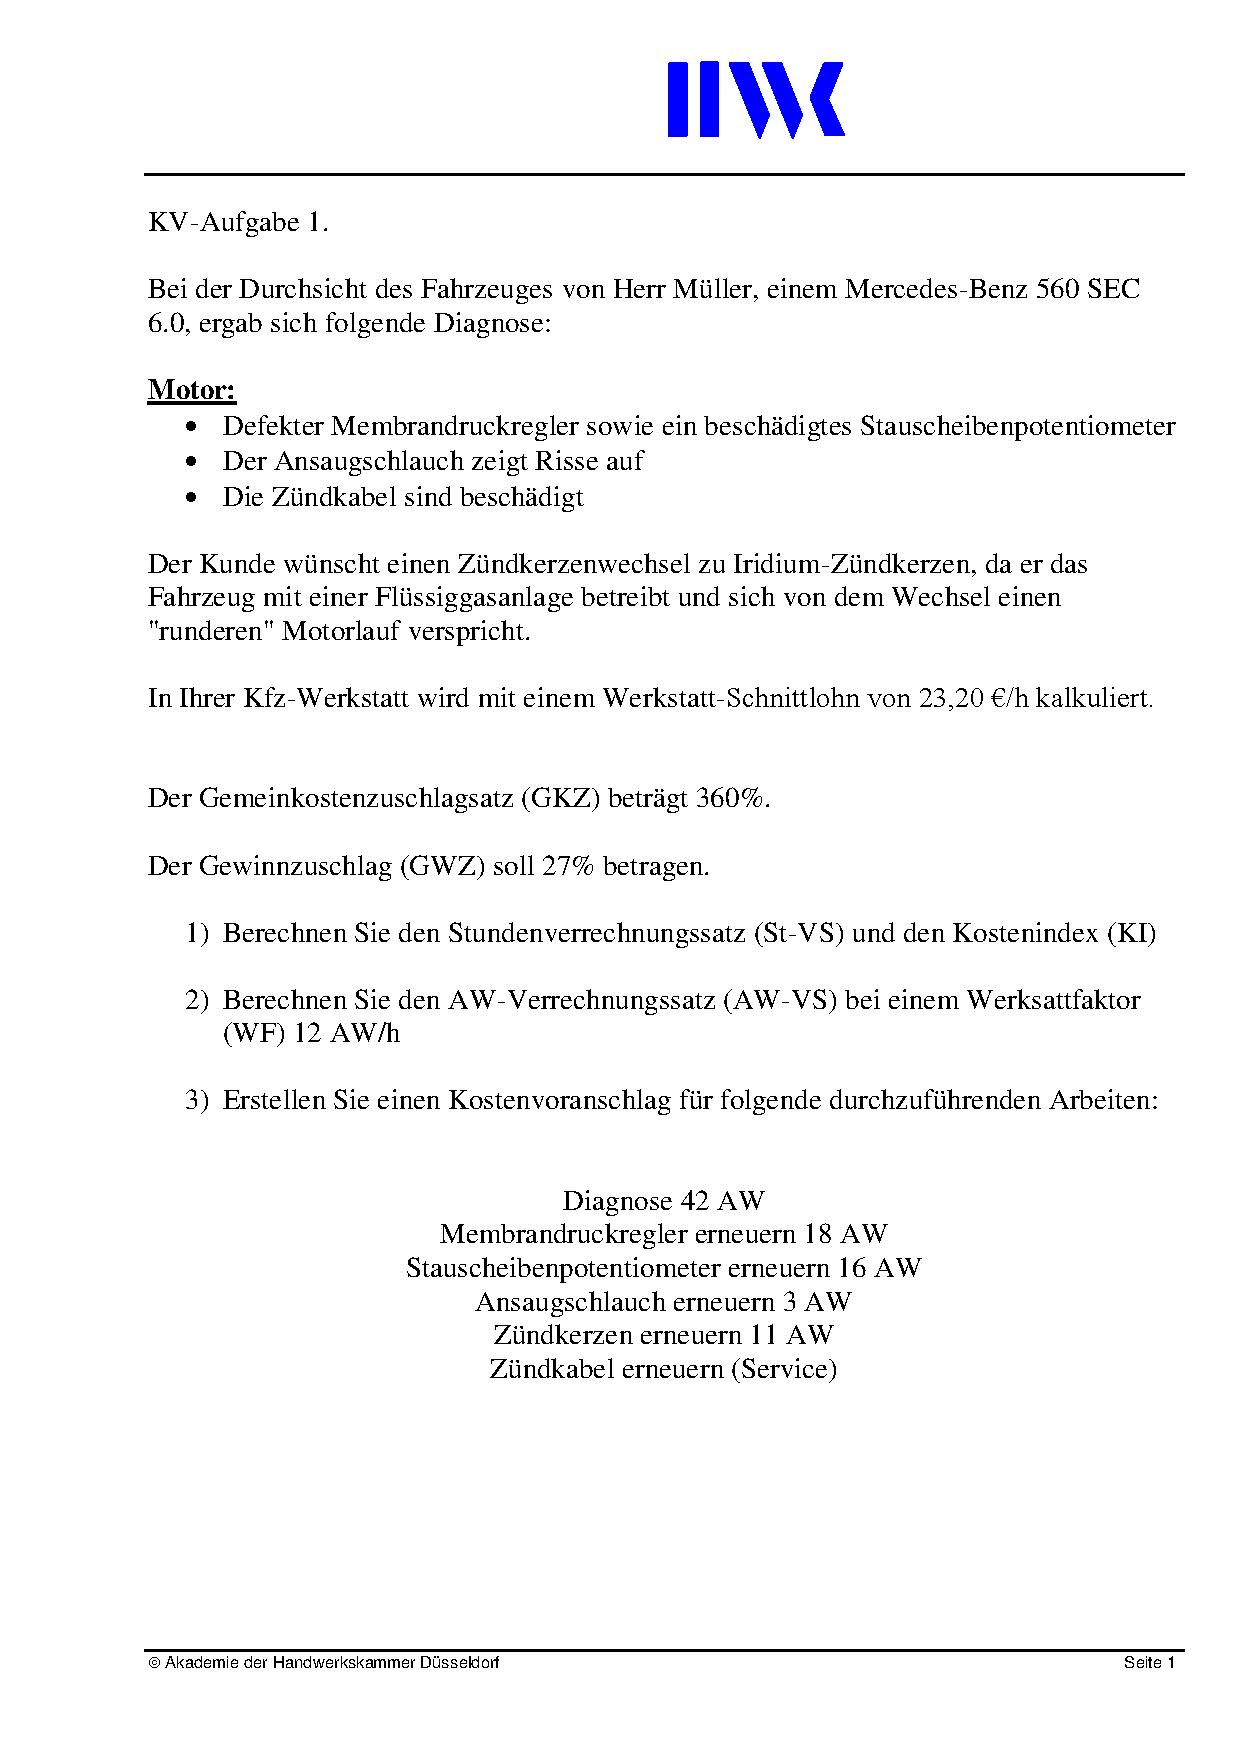
\includepdf[pages=-]{Tabellen/PDF/U07-Aufgabe-KV1-Stauscheibenpoti-AT.pdf}
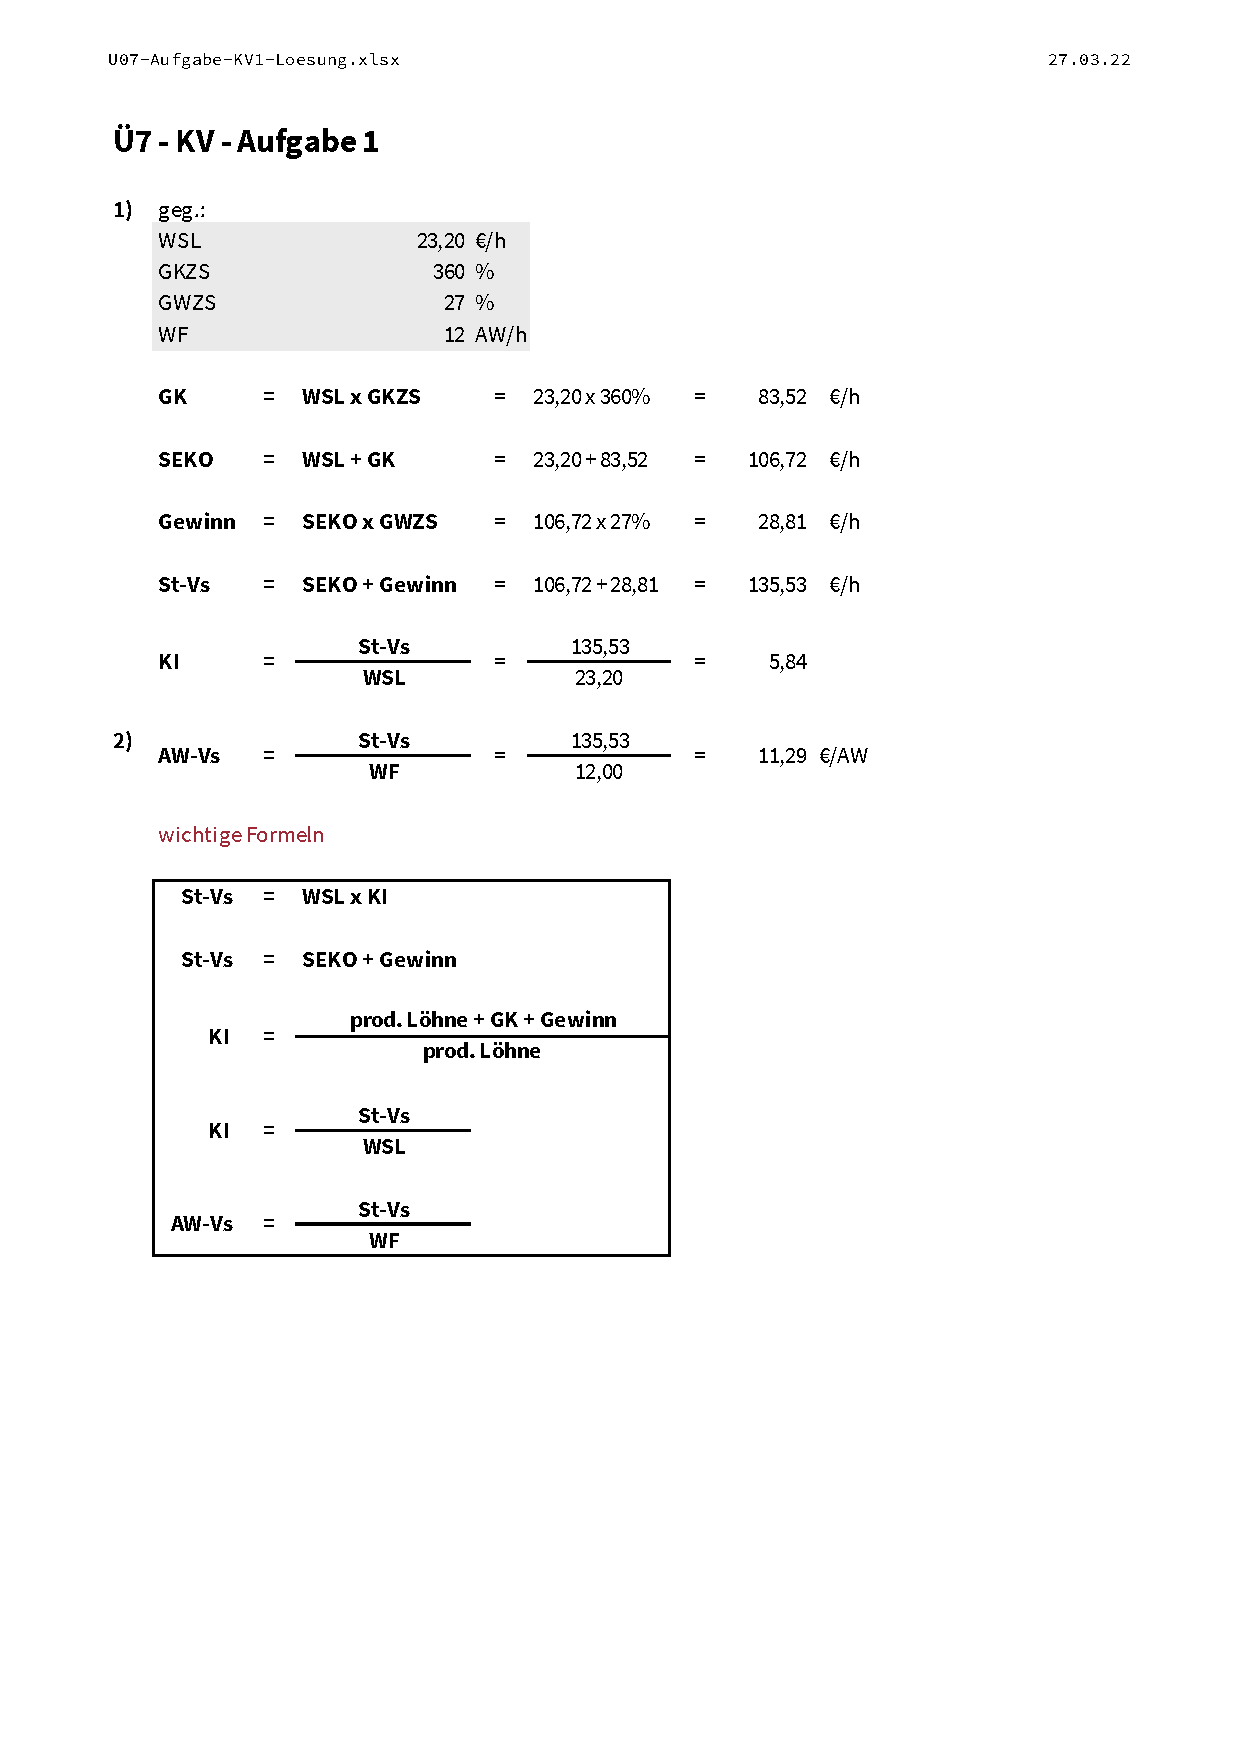
\includepdf[pages=-]{Tabellen/PDF/U07-Aufgabe-KV1-Loesung.pdf}

% -------
\section{U08 - Aufgabe - KV2 - HFM}\label{sec:U08-Aufgabe-KV2-HFM}\index{U08-Aufgabe-KV2-HFM}
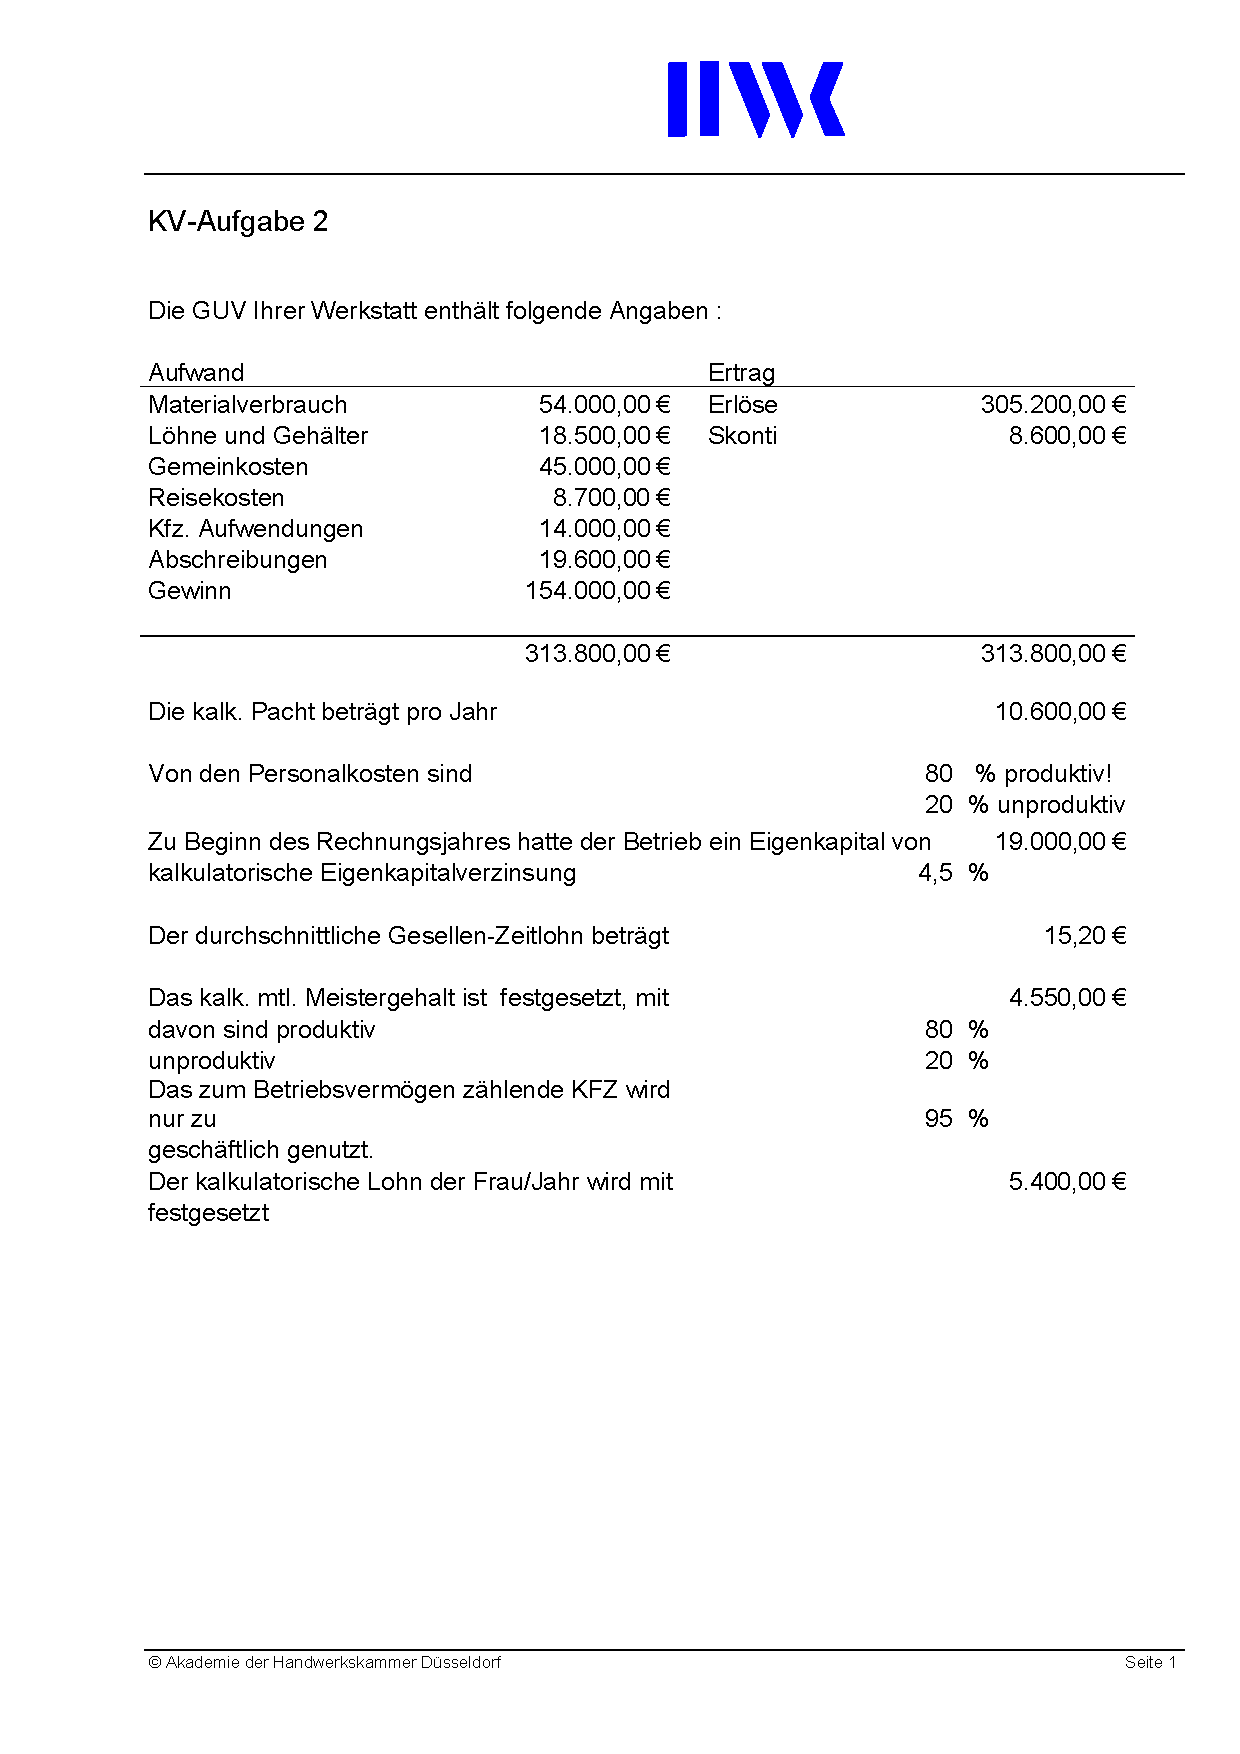
\includepdf[pages=-]{Tabellen/PDF/U08-Aufgabe-KV2-HFM.pdf}
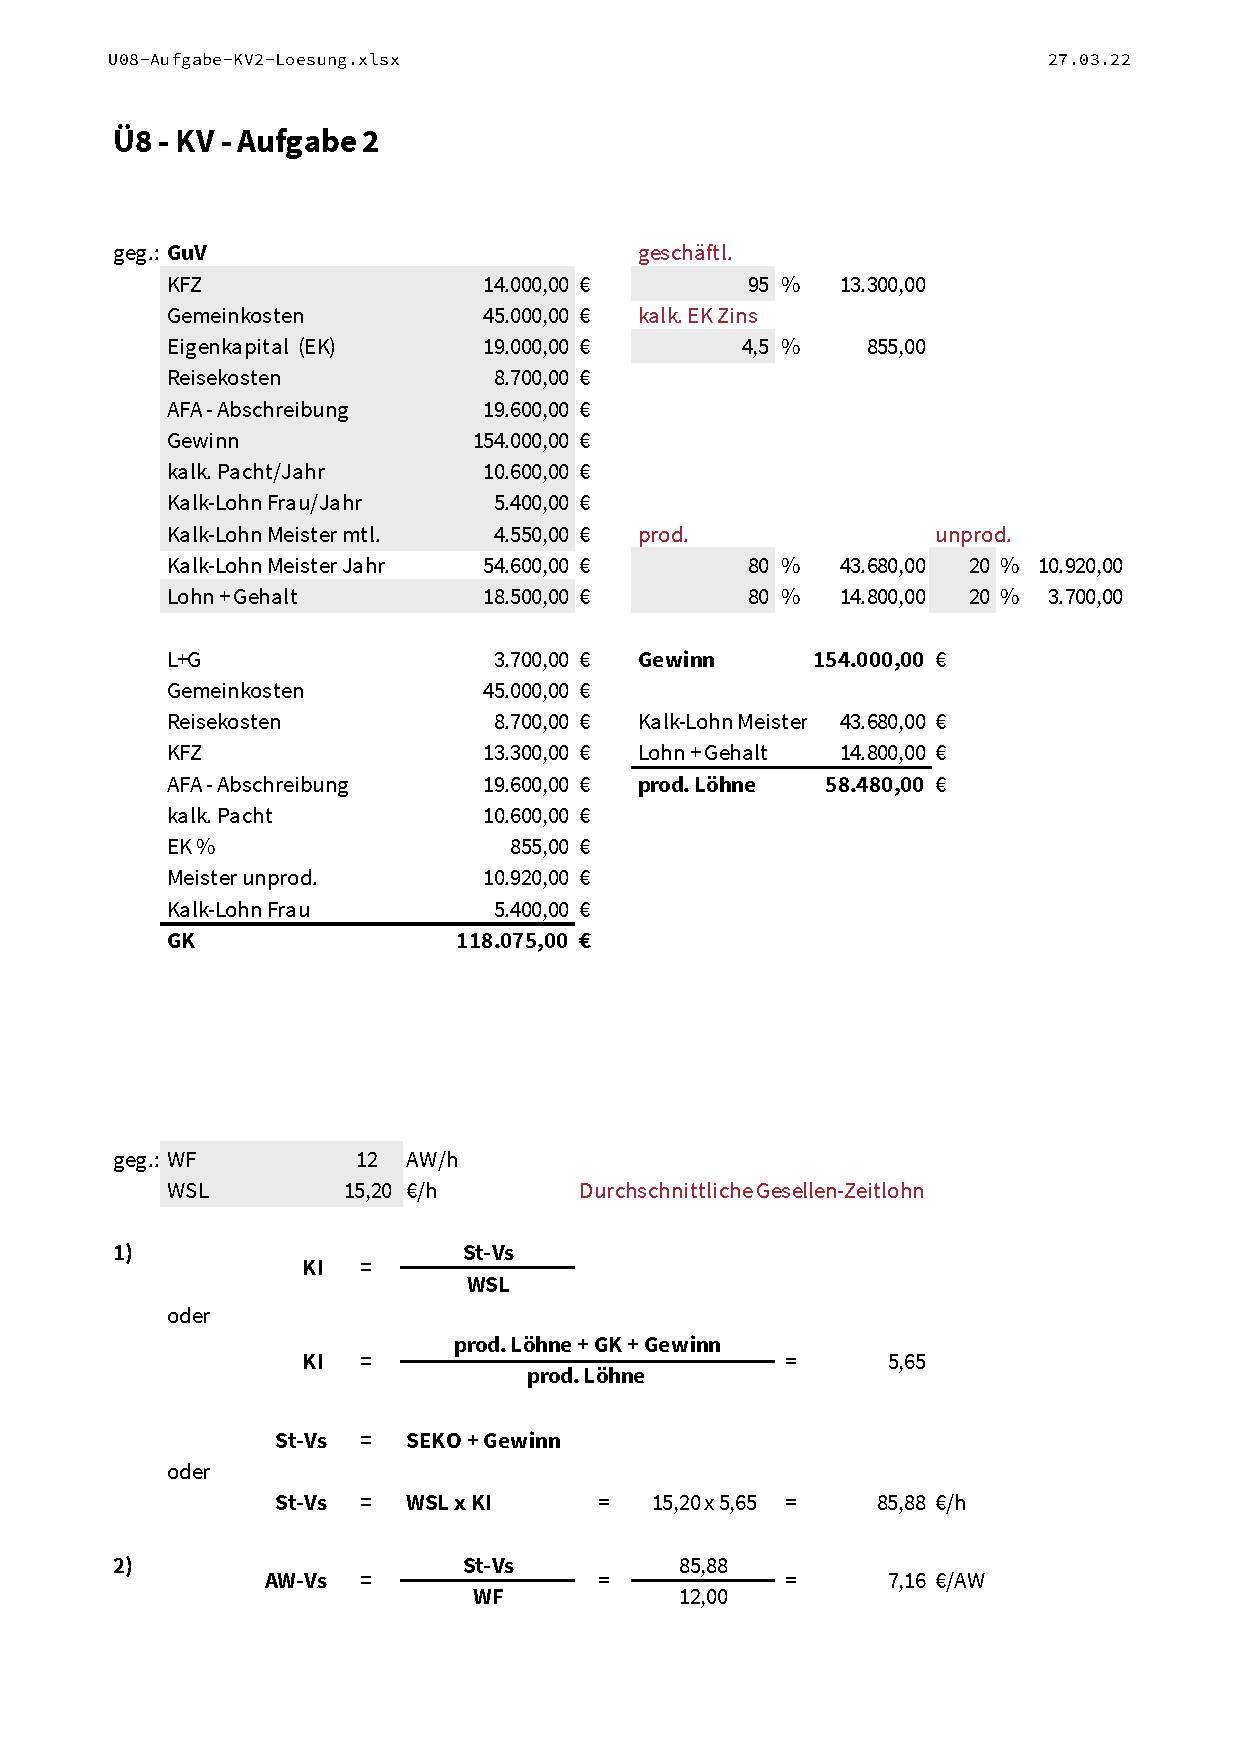
\includepdf[pages=-]{Tabellen/PDF/U08-Aufgabe-KV2-Loesung.pdf}

% -------
\section{U09 - Aufgabe - KV3}\label{sec:U09-Aufgabe-KV3}\index{U09-Aufgabe-KV3}
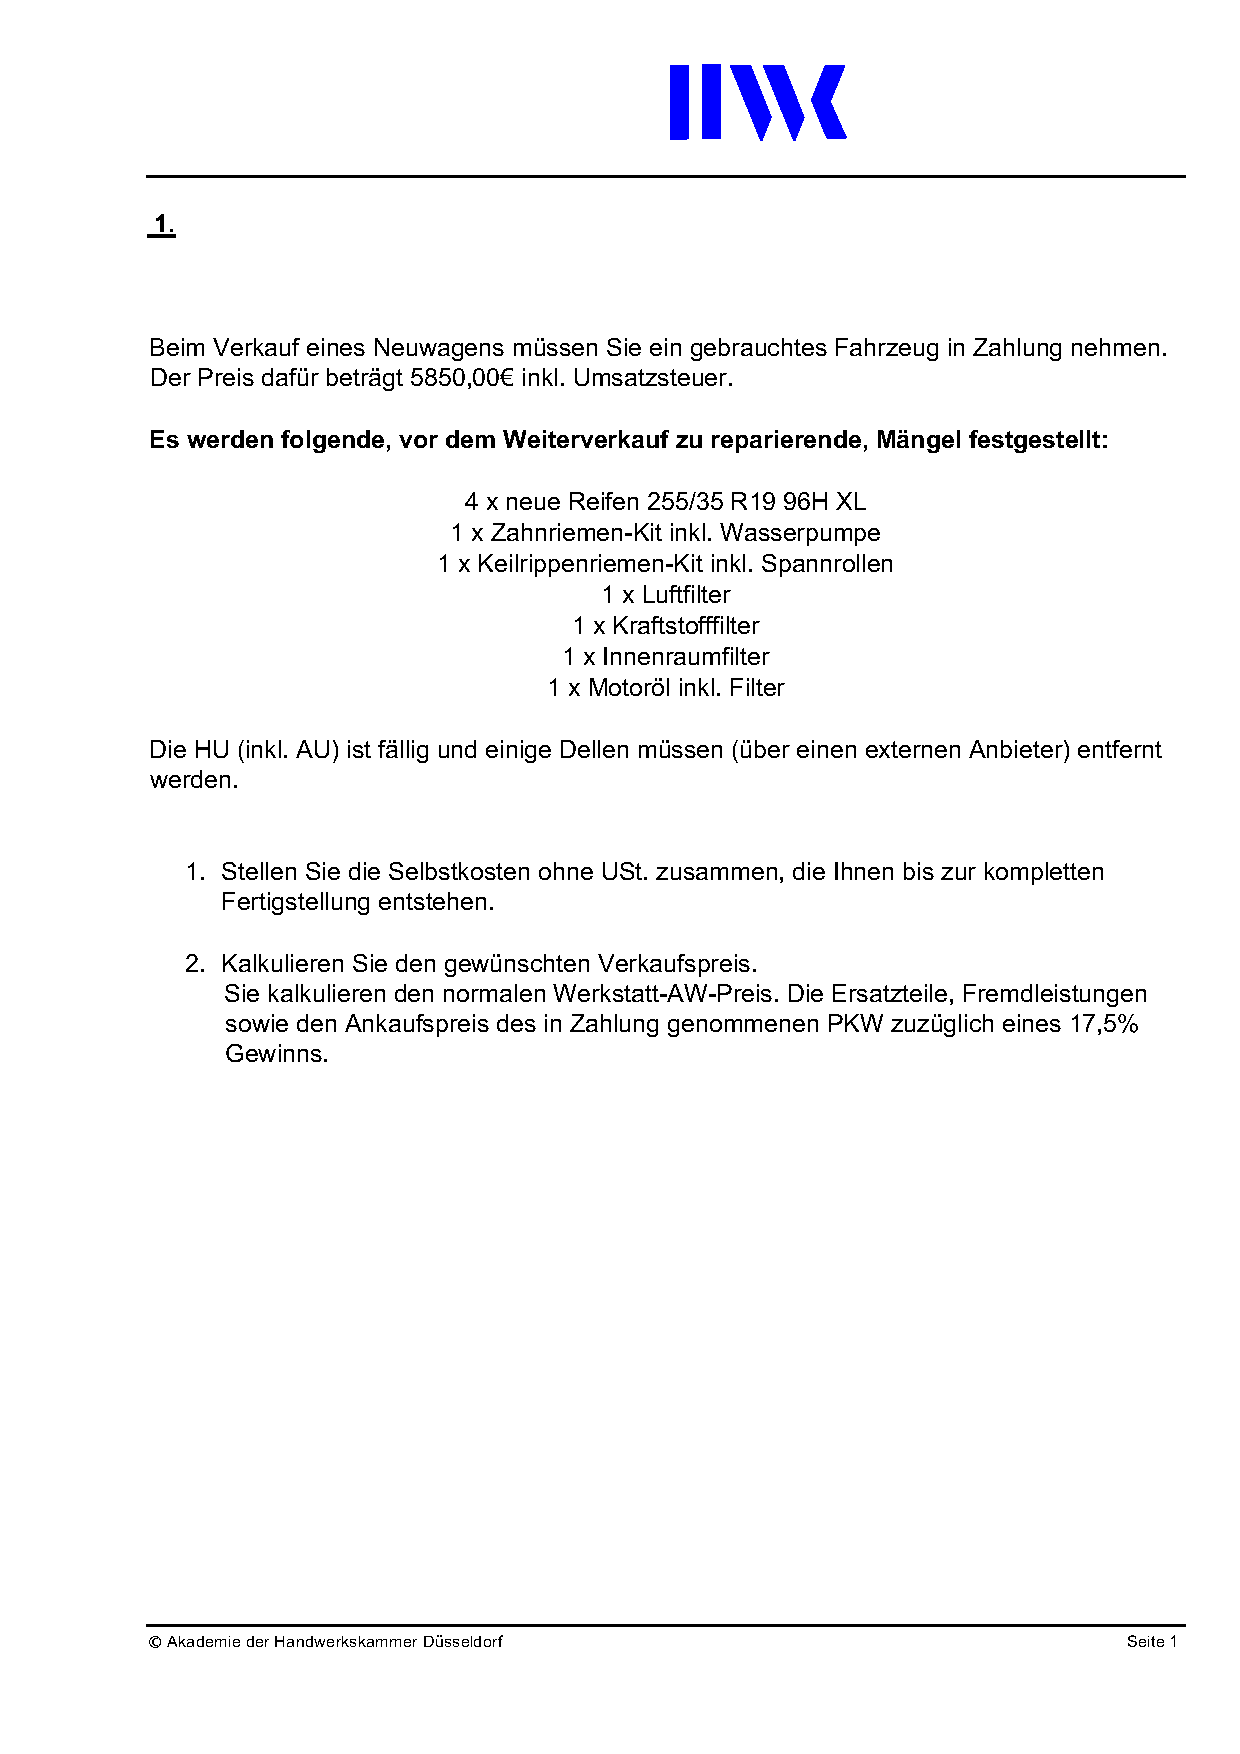
\includepdf[pages=-]{Tabellen/PDF/U09-Aufgabe-KV3.pdf}
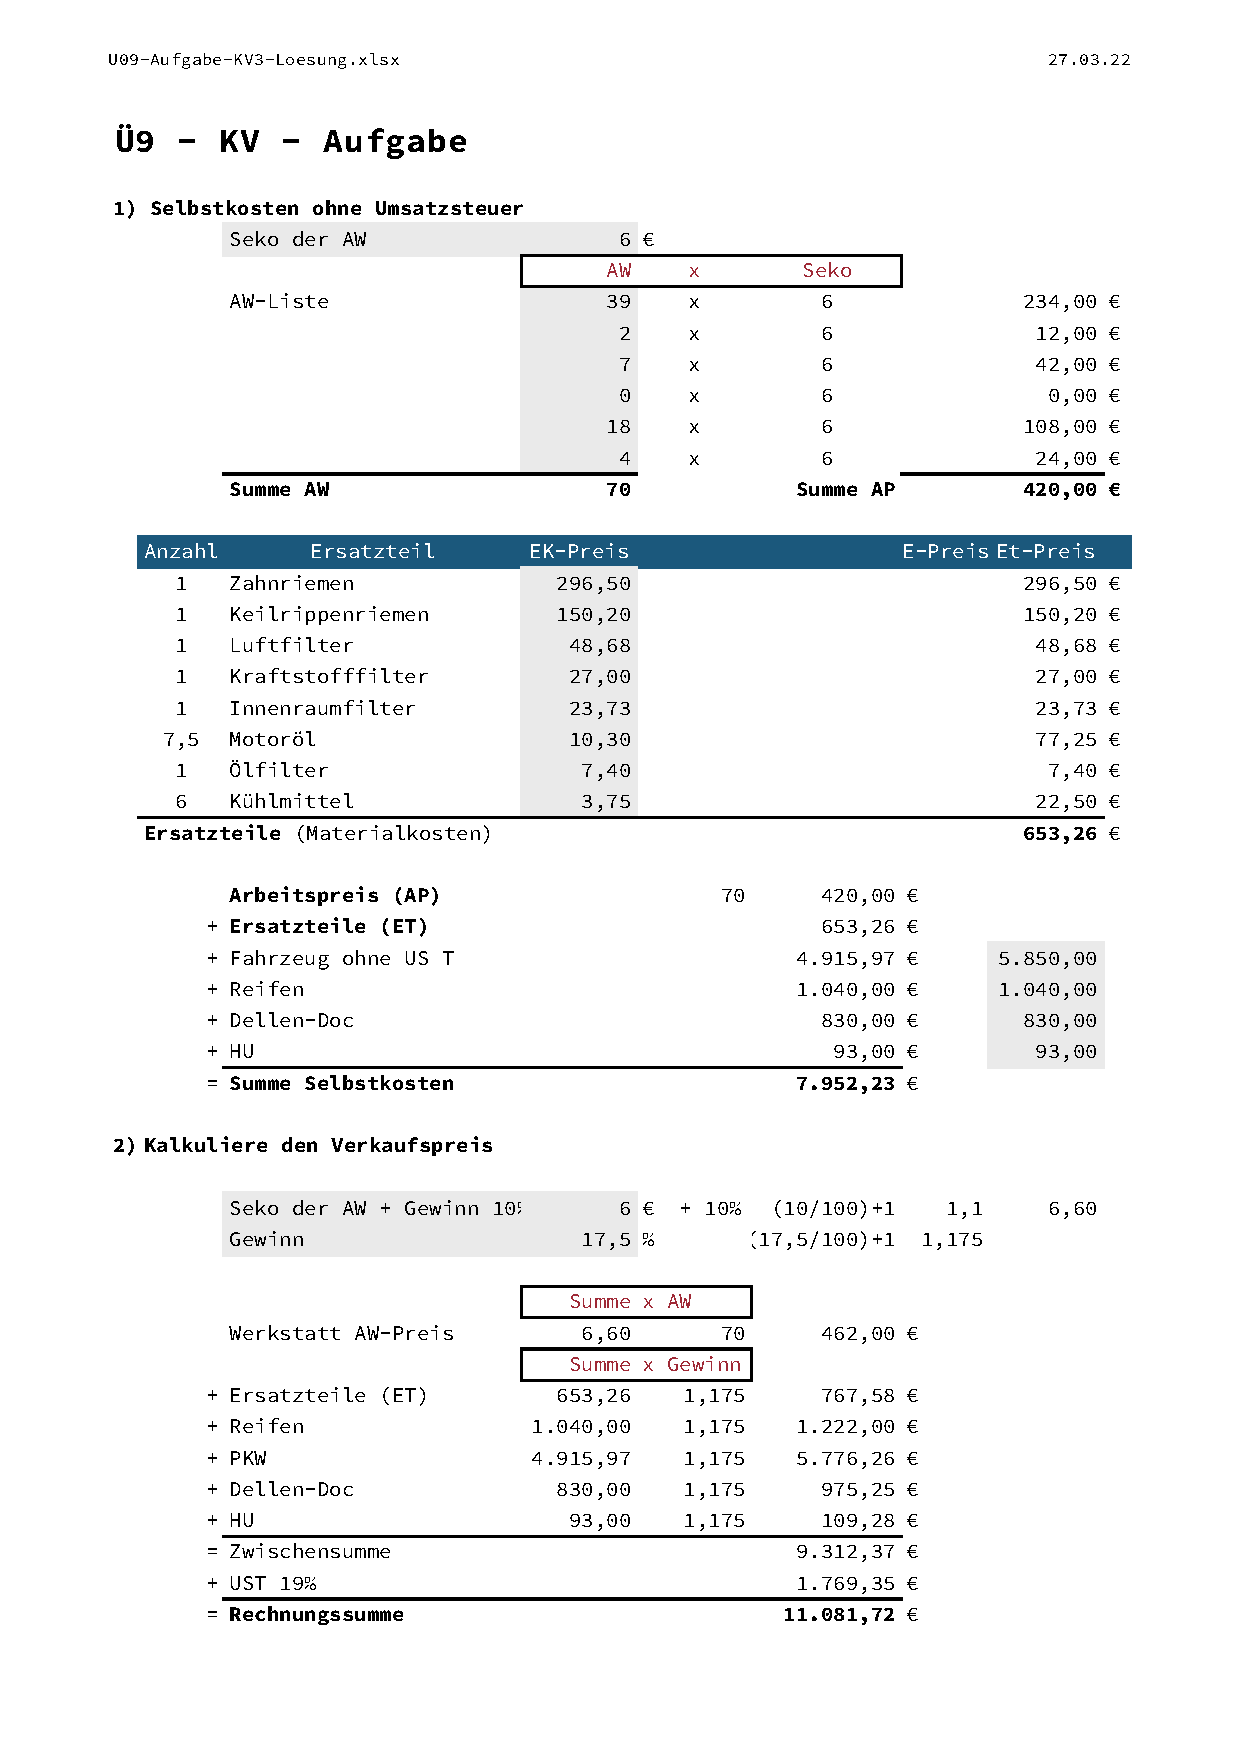
\includepdf[pages=-]{Tabellen/PDF/U09-Aufgabe-KV3-Loesung.pdf}

% -------
\section{U10 - Prüfungsaufgabentraining}\label{sec:U10-Pruefungsaufgabentraining}\index{U10-Pruefungsaufgabentraining}
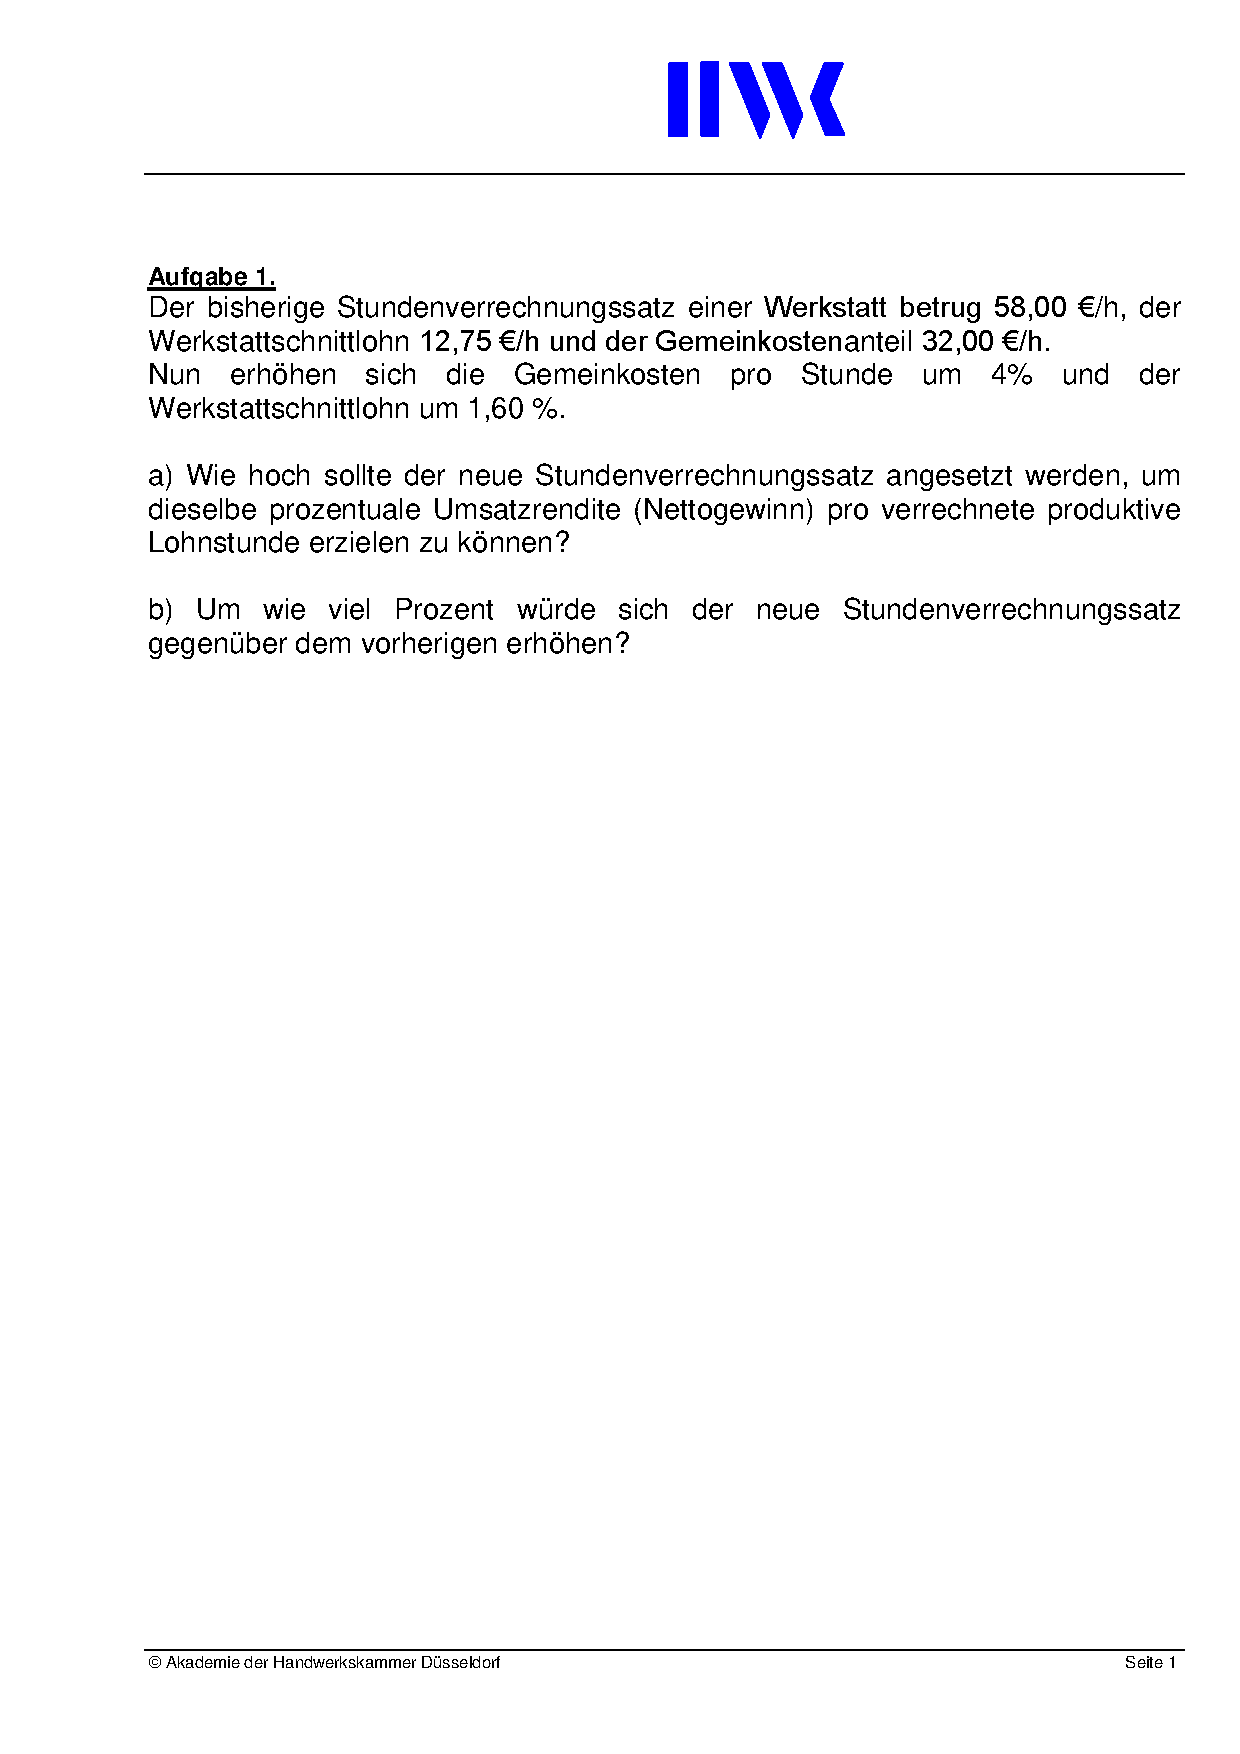
\includepdf[pages=-]{Tabellen/PDF/U10-Pruefungsaufgabentraining.pdf}
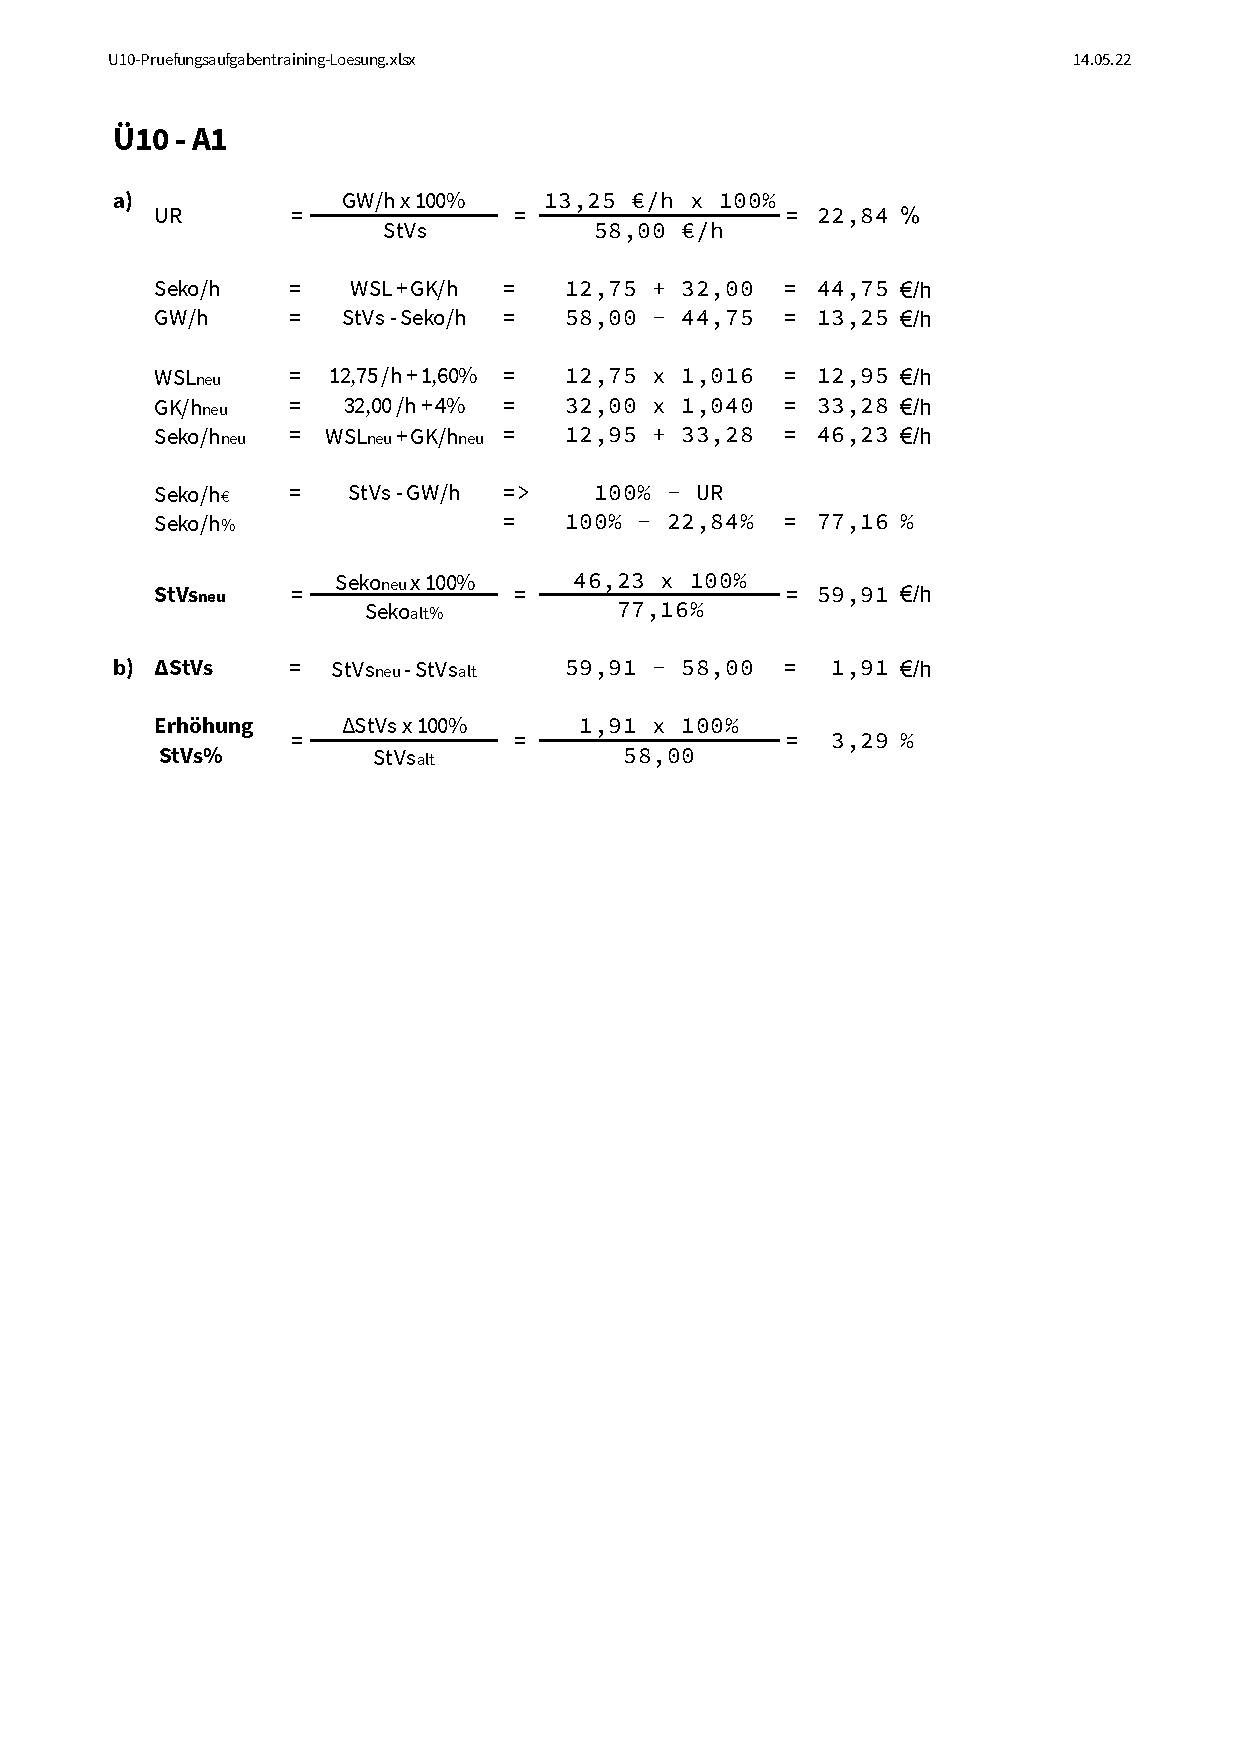
\includepdf[pages=-]{Tabellen/PDF/U10-Pruefungsaufgabentraining-Loesung.pdf}

% -------
\section{U11 - Aufgabe - Afa}

siehe Script

% -------
\section{U12 - Aufgabe - Leistungslohnsatz}\label{sec:U12-Aufgabe-Leistungslohnsatz}\index{U12-Aufgabe-Leistungslohnsatz}
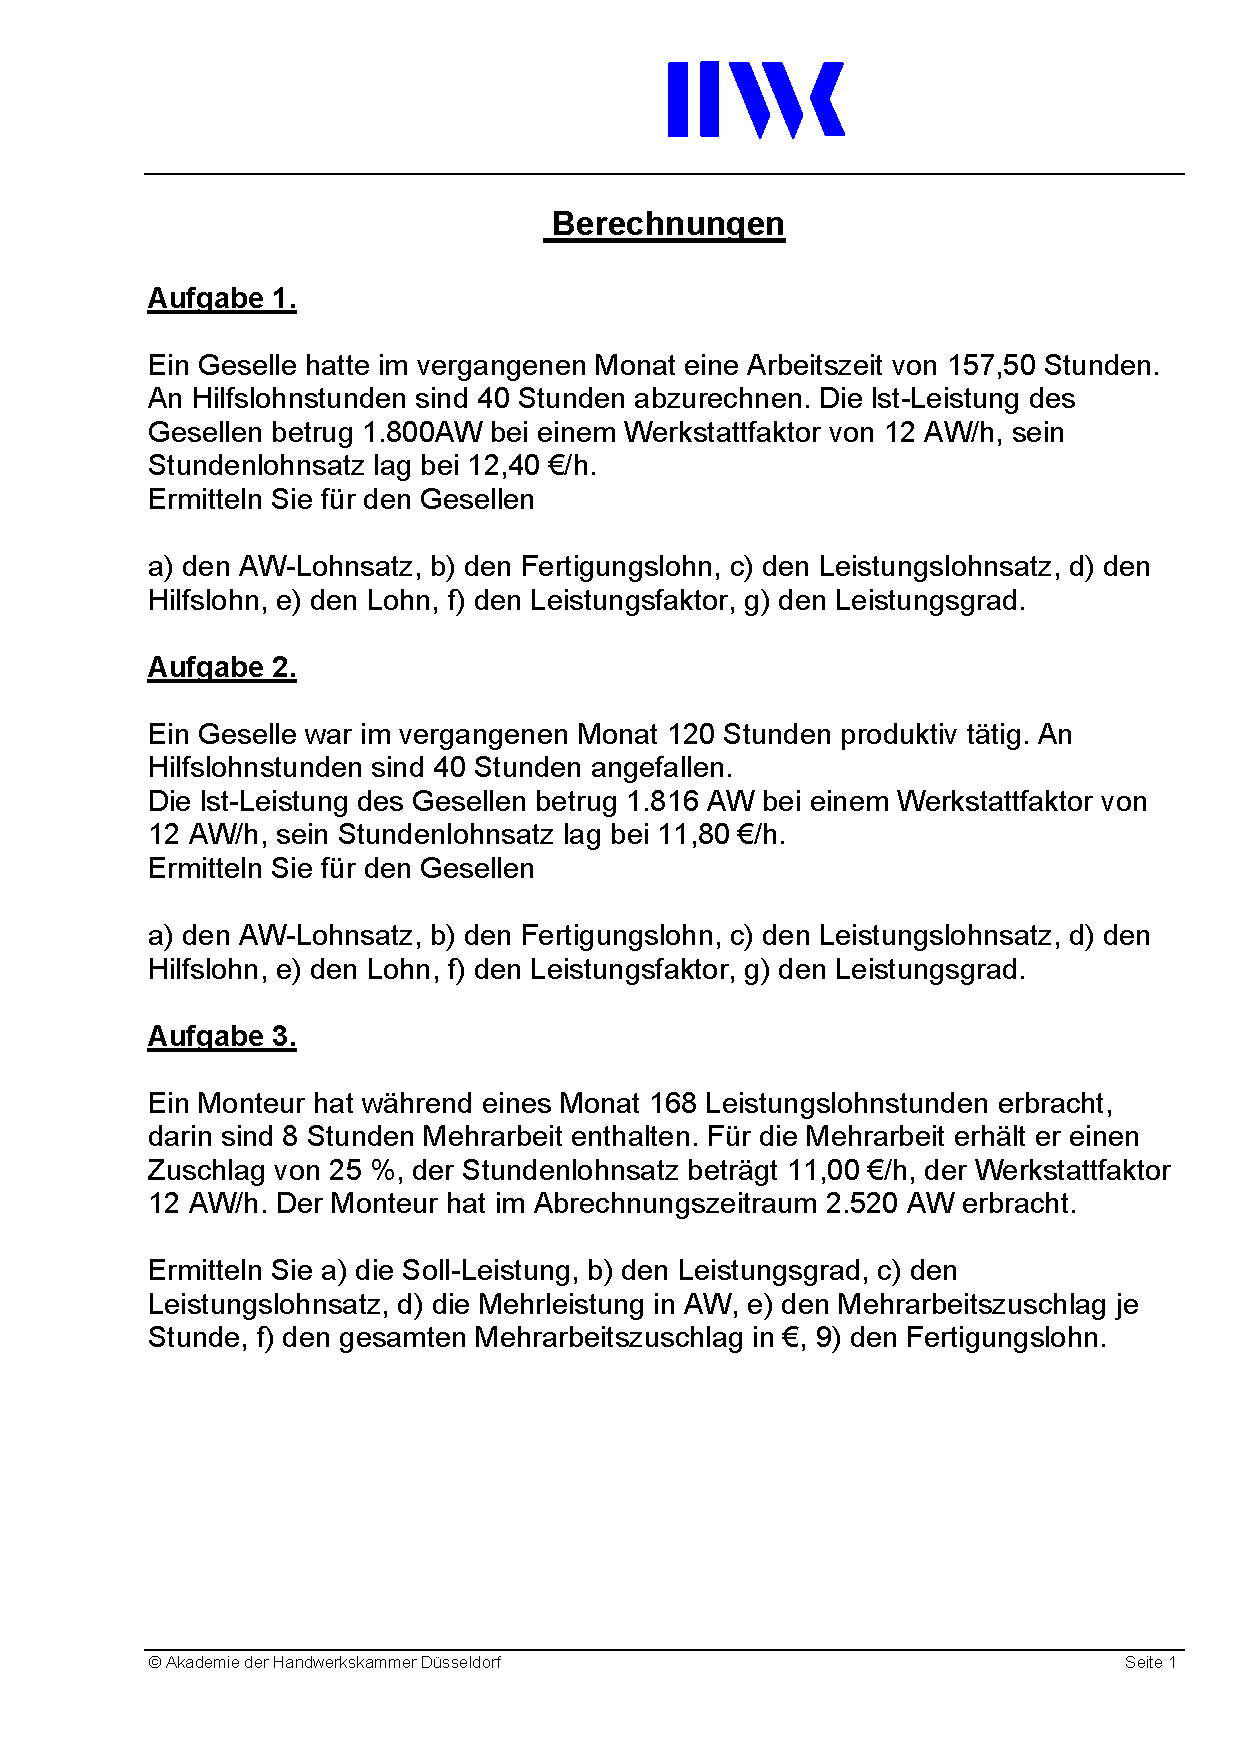
\includepdf[pages=-]{Tabellen/PDF/U12-Aufgabe-Leistungslohnsatz.pdf}
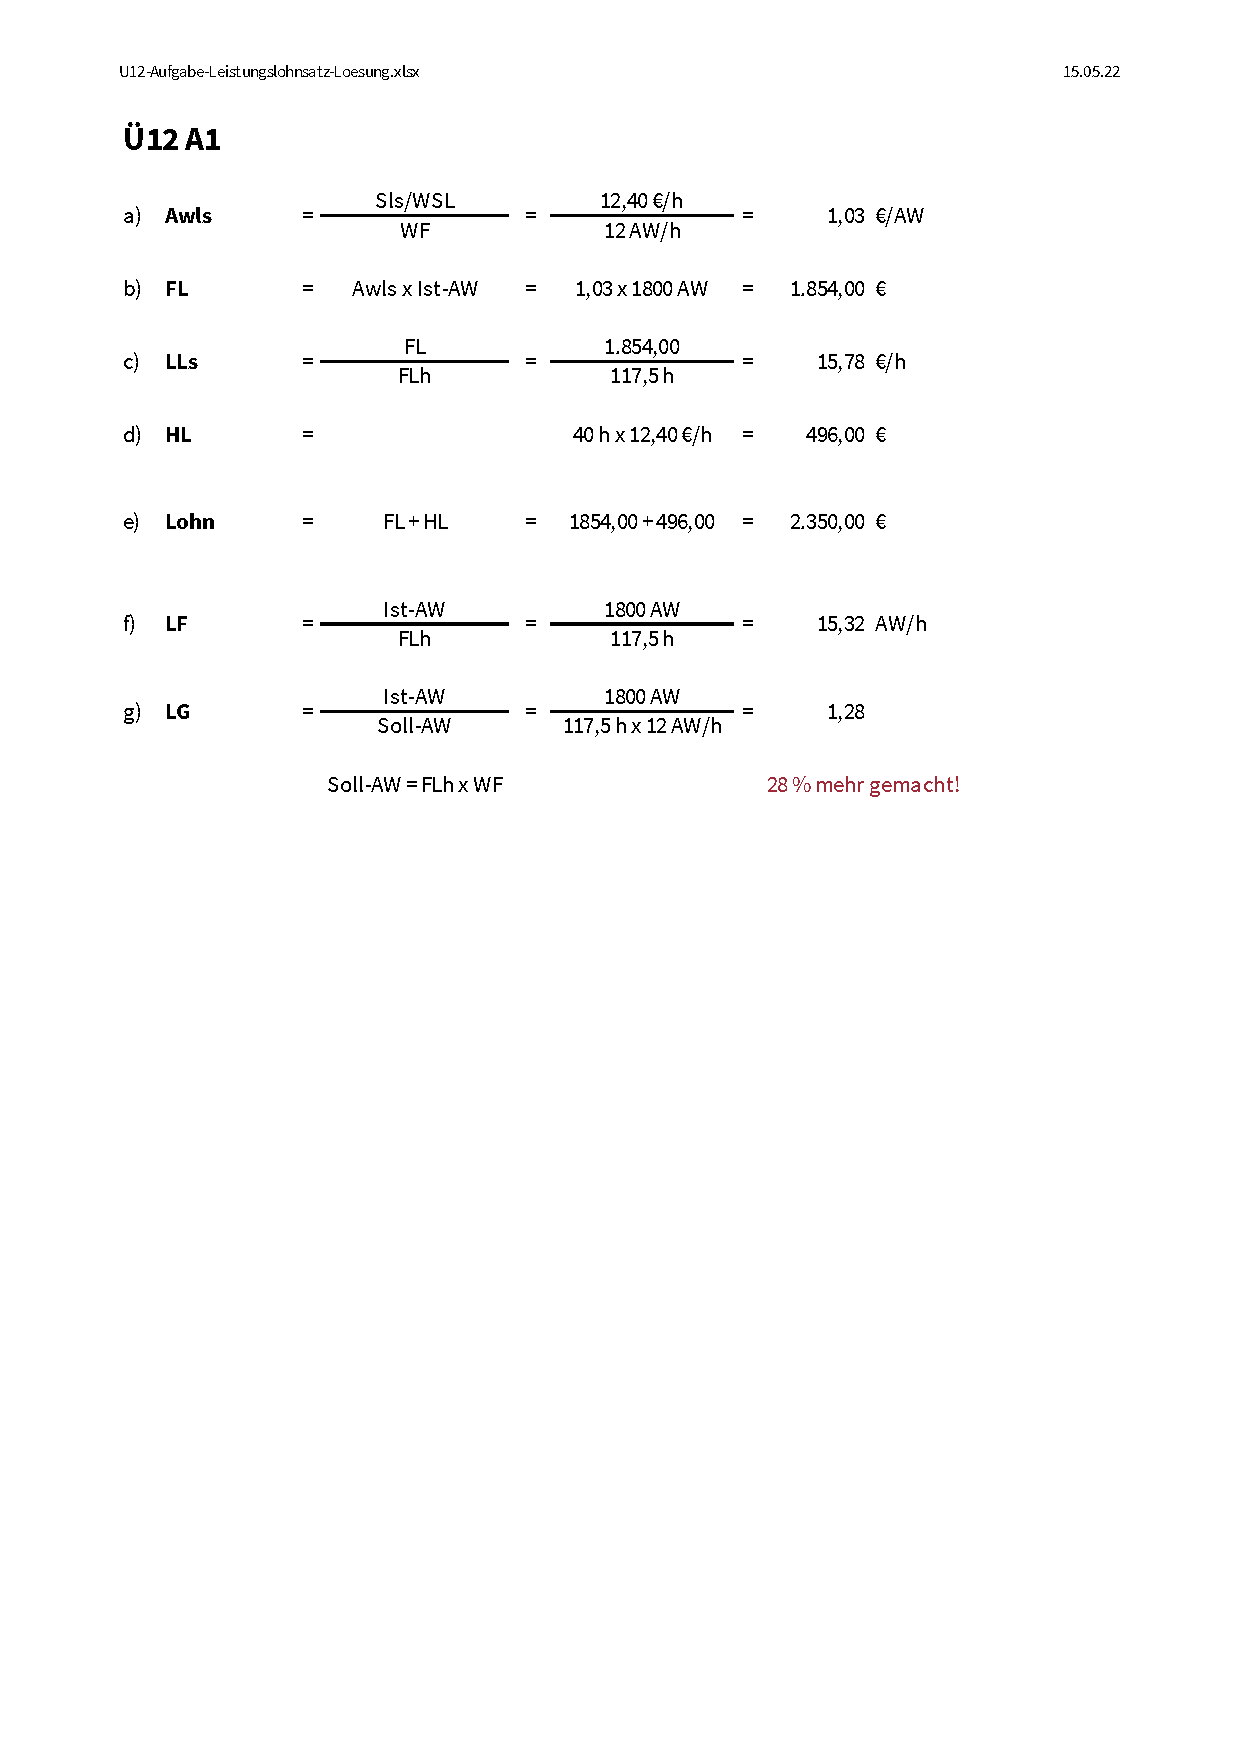
\includepdf[pages=-]{Tabellen/PDF/U12-Aufgabe-Leistungslohnsatz-Loesung.pdf}

% -------
\section{U13 - Kundenblätter - test Lösung}\label{sec:U13-Kundenblaetter-test-Loesung}\index{U13-Kundenblaetter-test-Loesung}
%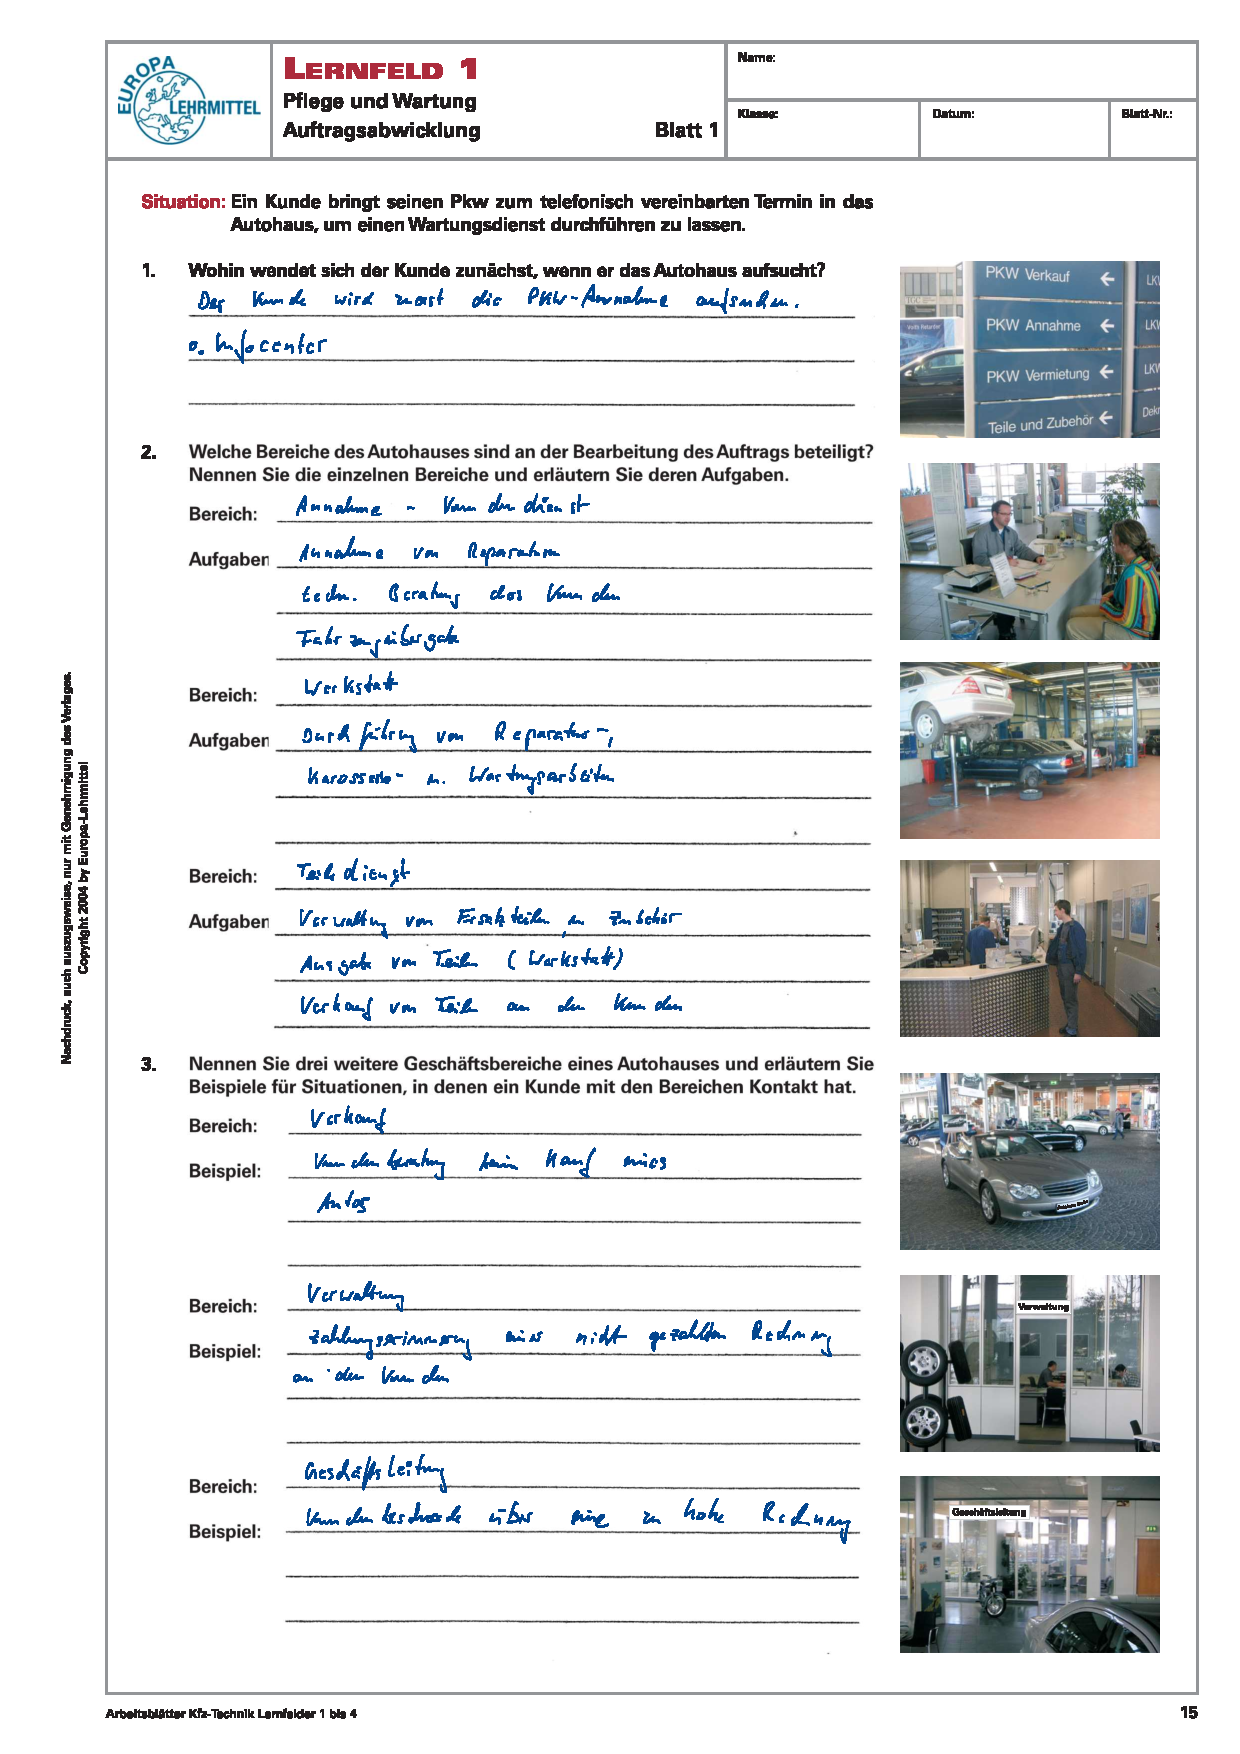
\includepdf[pages=-]{Tabellen/PDF/U13-Kundenblaetter-test-Loesung.pdf}

siehe Script









%%%%%%%%%%%%%%%%%%%%%%%%%%%%%%%%%%%%%%%%%%%%%%%%%%

% content/beispiele/tex/

%\chapter{Aufbau-der-Arbeit}
%%\chapter{Aufbau der Arbeit}

Jede Arbeit besteht in der Regel aus einer \textbf{Problemstellung}, einem \textbf{definitorischen Abschnitt}, der eigentlichen \textbf{Behandlung der Problemstellung} sowie einer \textbf{Zusammenfassung der zentralen Ergebnisse}.

\begin{description}

	\item[Einleitung] Im Zentrum des erstens Teils stehen die Darstellung des Themas der Arbeit und die genaue Auflistung der Fragestellungen (Wieso ist das Thema relevant?). Ebenso sollten schon einzelne Aspekte des Problems herausgearbeitet werden. Dabei ist es hilfreich, die zentralen Fragen aufzulisten, die im Rahmen der Arbeit beantwortet werden sollen.
	
	Außerdem sollte ein knapper Überblick gegeben werden, in welchen Schritten die Problembehandlung erfolgt: Hinführung zum Thema, Herleitung und Ausformulierung der Fragestellung, Abgrenzung des Themas (Angabe von Aspekten, die zum Thema gehören, aber ausgeklammert werden) und Aufbau der Arbeit (Begründung der Gliederung).
	
	\item[Grundlagen (definitorischer Teil)] Im zweiten Teil sollen zentrale Begriffe definiert und eingeordnet werden. Es geht dabei nicht darum, Definitionen aus Lexika zu suchen; stattdessen sollten problemorientierte Definitionen verwendet werden. Häufig können einzelne Begriffe unterschiedlich weit oder eng definiert werden, sodass auch eine Diskussion unterschiedlicher Definitionsansätze hilfreich sein kann, bevor eine für die weitere Arbeit verbindliche Definition gewählt wird. Zudem sollte ein Überblick über die in der Literatur vorhandenen Methoden bzw. Lösungsansätze, der aktuelle Stand der Technik und verwandte Arbeiten gegeben werden.
	
	\item[Hauptteil] Im Hauptteil der Arbeit (der in der Gliederung selbstverständlich nicht so zu benennen ist\ldots) erfolgt die eigentliche eigentliche Auseinandersetzung mit der Problemstellung. In diesem Teil kommt es darauf an, nicht nur Lehrbuchwissen zusammenzutragen, sondern die Problemstellung reflektiert zu bearbeiteten. Aussagen sollten durch herangezogene Literatur gestützt und belegt werden. Bitte darauf achten, in logischen, nachvollziehbaren Schritten vorzugehen.
	
	\item[Schlussbetrachtung] Die Antwort auf die in der Problemstellung aufgeworfenen Fragen soll kurz und prägnant zusammengefasst werden. Ebenso sollte ein Ausblick auf offen gebliebene Fragen sowie auf interessante Fragestellungen, die sich aus der Arbeit ergeben, gegeben werden. Eine kritische Betrachtung der eigenen Arbeit ist an dieser Stelle ebenfalls sinnvoll.

\end{description}

\noindent
Eine Sammlung unserer Tipps für das Schreiben von Ausarbeitungen befindet sich online unter \url{https://www.dcl.hpi.uni-potsdam.de/media/theses/}.

%\chapter{LaTeX-Beispiel-beamer}
%% ju 23-Jul-21
\section*{Einleitung}

\emph{Sonderzeichen}  wie <<\& oder \%>> müssen mit einem Backslash \verb|\& oder \%| maskiert werden, 
damit sie von LaTeX nicht als Befehle missverstanden werden.


\emph{Website} \footnote{\url{https://golatex.de/wiki/Hauptseite}} \verb|\footnote{\url{https://golatex.de/wiki/Hauptseite}}| 

\emph{PDF Datei einbinden} \verb|
\includepdf[landscape=false]{images/logo.eps}| 

\includepdf[landscape=false]{images/logo.eps} 

\clearpage
\subsection*{Stand der Forschung}

Während die traditionelle Latexproduktion bereits hinreichend erforscht ist (\autoref{fig:latex}) \\
\verb|(\autoref{fig:latex})|, bleibt das wissenschaftliche Verständnis elektronischer Verarbeitungsprozesse dieses 
vielseitigen Materials weiterhin lückenhaft. 


\begin{figure}[!ht]% hier: !ht
	\centering
	
\includegraphics[width=0.25\textwidth]{images/logo.eps}
	\caption{Traditionelle Latexproduktion}\label{fig:latex}%
\end{figure}

\lstset{language=TeX}% C, TeX, Bash, Python 
\begin{lstlisting}[
	%caption={}, label={code:}%% anpassen
]
% Optionen
scale = Wert, Vergrösserungsfaktor
width/height = Wert für die Einstellung der Breite/Höhe
angle = Wert, Winkel (in Grad)
b = bottom - Seitenende 
t = top - Seitenanfang
h = here
p = page - komplette Seite  
% Abbildung
\begin{figure}[!ht]% hier: !ht
	\centering
	
\includegraphics[width=0.25\textwidth]{images/logo.eps}
	\caption{Traditionelle Latexproduktion}\label{fig:latex}%
\end{figure}
\end{lstlisting}


\clearpage
\section*{Methodik}

Unter Zuhilfenahme der Formeln \autoref{eq:ekin} \verb|\autoref{eq:ekin}| und \autoref{eq:impuls} \verb|\autoref{eq:impuls}| werden wir 
diese Forschungslücke schließen.  
$E_{kin}$ \verb|$E_{kin}$| ist die kinetische Energie, $m$ \verb|$m$| die Masse und $\vec{v}$ \verb|$\vec{v}$| die Geschwindigkeit.

Wurzel $\sqrt{2}$ \verb|$\sqrt{2}$|

Bruch $\frac{\text{Zähler}}{\text{Nenner}}$ \verb|$\frac{\text{Zähler}}{\text{Nenner}}$|

\begin{equation}
	\label{eq:ekin}% 
	\sum E_{kin} = \sum E'_{kin}
\end{equation}

\begin{equation}
	\label{eq:impuls}% 
	\vec{v_1} - \vec{v_1'} = \frac{m_2}{m_1} (\vec{v_2'} - \vec{v_2})
\end{equation}

\lstset{language=TeX}% C, TeX, Bash, Python 
\begin{lstlisting}[
	%caption={}, label={code:}%% anpassen
]
% Mathe
\begin{equation}
	\label{eq:ekin}% 
	\sum E_{kin} = \sum E'_{kin}
\end{equation}
\end{lstlisting}


\clearpage
\section*{Ausblick}

Daraus ergeben sich gemäß (\autoref{tab:schritte}) \verb|(\autoref{tab:schritte})| folgende nächste Schritte, 
deren sequenzielle Ausführung von essenzieller Bedeutung ist.

\begin{table}[!ht]% hier: !ht
	\centering
	\begin{tabular}{@{}cl@{}}% lcr
		\toprule
		\textbf{Nr.} & \textbf{Vorgehen} \\
		\midrule
		1 & Aktuellen Forschungsstand recherchieren \\
		2 & Methoden entwickeln \\
		3 & Schlussfolgerung aufstellen \\
		\bottomrule
	\end{tabular}
	\caption{Nächste Schritte}\label{tab:schritte}
\end{table}

\clearpage
\lstset{language=TeX}% C, TeX, Bash, Python 
\begin{lstlisting}[
	%caption={}, label={code:}%% anpassen
]
% Tabelle
\begin{table}[!ht]% hier: !ht
	\centering
	\begin{tabular}{@{}cl@{}}% lcr
		\toprule
		\textbf{Nr.} & \textbf{Vorgehen} \\
		\midrule
		1 & Aktuellen Forschungsstand recherchieren \\
		2 & Methoden entwickeln \\
		3 & Schlussfolgerung aufstellen \\
		\bottomrule
	\end{tabular}
	\caption{Nächste Schritte}\label{tab:schritte}
\end{table}
\end{lstlisting}
%\chapter{Latex-install-Ubuntu}
%% letztes Update: 27-Jul-20
Quelle: Dr.~Uwe Ziegenhagen -- Anleitung zur TEX Live Installation

\section{TEX Live Download}\label{tex-live-download}

Download \footnote{\url{http://mirror.ctan.org/systems/texlive/tlnet}}

Download-texlive vgl.~(\autoref{code:Download-texlive}).

\lstset{language=C}% C, TeX, Bash, Python 
\begin{lstlisting}[%% anpassen
caption={Download-texlive},label={code:Download-texlive}
]
cd Downloads
tar xvfz install-tl-unx.tar.gz
cd install-tl-20200114
perl install-tl
perl install-tl -gui
\end{lstlisting}

\section{TeX Version}\label{tex-version}

tex --version

\section{TEX Live Installation}\label{tex-live-installation}

Install-texlive vgl.~(\autoref{code:Install-texlive}).

\lstset{language=C}% C, TeX, Bash, Python 
\begin{lstlisting}[%% anpassen
caption={Install-texlive},label={code:Install-texlive}
]
sudo apt install texlive texlive-latex-recommended texlive-fonts-recommended \
    texlive-latex-base texlive-base texlive-latex-extra texlive-lang-german

# Verbesserte Schriftarten bei T1-Kodierung
sudo apt-get install cm-super 
\end{lstlisting}

\section{Umgebungsvariablen für
Unix}\label{umgebungsvariablen-fuer-unix}

Umgebungsvariable vgl.~(\autoref{code:Umgebungsvariable}).

\lstset{language=C}% C, TeX, Bash, Python 
\begin{lstlisting}[%% anpassen
caption={Umgebungsvariable},label={code:Umgebungsvariable}
]
vi ~/.profile
# Datei 
PATH=/usr/local/texlive/2019/bin/x86_64-linux:$PATH; export PATH
MANPATH=/usr/local/texlive/2019/texmf-dist/doc/man:$MANPATH; export MANPATH
INFOPATH=/usr/local/texlive/2019/texmf-dist/doc/info:$INFOPATH; export INFOPATH

sudo vi /etc/manpath.config
# Datei 
MANPATH_MAP /usr/local/texlive/2019/bin/x86_64-linux \
  /usr/local/texlive/2019/texmf-dist/doc/man  
\end{lstlisting}

%\chapter{Mathe-Aufgaben}
%
\textbf{Aufgabe 1:} \enspace Jasmin hat ihre Freunde Nico, Laura und Anna zum Geburtstag eingeladen. Nico will nicht kommen, wenn Laura nicht kommt. Laura und Anna kommen beide oder kommen beide nicht. Aber Anna sagt: >>Wenn Nico und Laura beide nicht kommen, dann komme ich.<< Wer von den dreien wird unter diesen Bedingungen tatsächlich zum Geburtstag erscheinen?


\textbf{Aufgabe 2:} \enspace In der Anwaltsserie >>Suits<< (Staffel 4, Folge 1) kommt es zu Folgendem Gespräch zwischen Mike und seiner Sekräterin Amy.


\begin{enumerate}[label={\protect\ding{\value*}},start=192]
    \item Amy: >>Und wie lief dein Treffen mit dem geheimnisvollen Harvey Specter?<<
    \item Mike: >>Ein Arsch zu sein macht einen nicht geheimnisvoll.<<
    \item Amy: >>Na dann bist du ja ein ganz offenes Buch.<<
\end{enumerate}

Untersuchen Sie das Gespräch aussagenlogisch und prüfen Sie den Wahrheitswert von Amys Aussage.


\textbf{Aufgabe 3:} \enspace Formalisieren Sie die folgenden Aussagen und verneinen Sie sie anschließend (ohne das Wort nicht davor zu setzen) und übersetzen Sie wieder in Umgangssprache:

\begin{enumerate}[label=(\alph*)]
    \item Volksmund: >>Bei Nacht sind alle Katzen grau.<<
    \item Plakatwerbung: >>Wenn einer hochguckt, dann gucken alle.<<
    \item Gorbatschov: >>Wer zu spät kommt, den bestraft das Leben.<<
\end{enumerate}

\textbf{Aufgabe 4:} \enspace Wurzel

\begin{multicols}{3}
    \begin{enumerate}[label=(\alph*)]
        \item $\sqrt{169}$
        \item $\sqrt{0,36}$
        \item $\frac{\sqrt{45}}{\sqrt{80}}$
        \item $\sqrt{32}$
        \item $\sqrt{2}$
        \item $\sqrt{1,44}$
        \item $\sqrt{\frac{75}{12}}$
    \end{enumerate}
\end{multicols}
%\chapter{Mathe-Latex}
%\section{\textbf{Text Unterstreichen}}
    \underline{wichtiger Text} und \emph{kursiver Text} und \textbf{fetter Text}

 
\section{\textsc{Kapitaelchen}}  
    Text in Grossbuchstaben setzen durch \LaTeX
    \begin{itemize} % \item[] avoids bullet
        \item[] Einen längeren Satz\\ einrücken.
    \end{itemize}

\section{Vor- und Nachteile}
    \begin{tabular}[h]{ll}
        {\textbf{Vorteile}}   &  {\textbf{Nachteile}} \\
        Argument 1            &  Argument 2 \\
        Argument A            &  Argument B \\
    \end{tabular} 

\section{Summe}
    \begin{tabular}[h]{clrr}
        & Betrag &               &  $1.000,00$ \\
    $-$ & Skonto & $2\%$         &     $20,00$ \\
        \hline
    $=$ & $\sum$ &               &    $980,00$  
    \end{tabular} 
    
\section{Division Zinsen}
    $
        \frac{\text{ Betrag } \cdot \text{ Prozentsatz } \cdot \text{ Zeit } }{100 \cdot \text{ Zeitgröße }} 
        = \frac{12.597,90 \cdot 12 \cdot 20 \text{ T } }{100 \cdot 360} 
        = 83,99 \text{ \euro }
    $

    \begin{align*}
        \frac{\text{ Betrag } \cdot \text{ Prozentsatz } \cdot \text{ Zeit } }{100 \cdot \text{ Zeitgröße }} 
        = \frac{12.597,90 \cdot 12 \cdot 20 \text{ T } }{100 \cdot 360} 
        = 83,99 \text{ \euro }
    \end{align*} 

\section{Tabelle 2}
    \begin{table}[!ht]% hier: !ht 
        \begin{tabular}{@{}lcr@{}}
        \toprule 
        \textbf{Großbuchstaben} & \textbf{Kleinbuchstaben} & \textbf{Name}\\
        \midrule
        21 \euro & 22000 & 230.000 \\
        $31$ \euro & $32000$ & $330.000$ \\
        \bottomrule
        \end{tabular}
    \end{table}

\section{Checkliste}
    Meine Liste
    \begin{itemize} \itemsep -2pt  % reduce space between items
        \item[$\Box$]   Punkt 1
        \item[$\Box$]   Aufgabe 2 
    \end{itemize}

    \begin{itemize}[label=\checkmark] \itemsep -2pt
        \item Check 1
        \item Check 2   
    \end{itemize}

\section{\textcolor{rot5}{Nenne 4x Lerzielstufen (Taxonomien)}}
    \begin{enumerate}[label={\protect\ding{\value*}},start=192]
        \item Reproduktion
        \item Reorganisieren
        \item Transfer
        \item Kreativ
    \end{enumerate}

\section{Wurzel berechnen}
    \begin{multicols}{3}
        \begin{enumerate}[label=(\alph*)]
            \item $\sqrt{169}$
            \item $\sqrt{0,36}$
            \item $\frac{\sqrt{45}}{\sqrt{80}}$
        \end{enumerate}
    \end{multicols}

\section{Aufgabe Logik}
    Formalisieren Sie die folgenden Aussagen und verneinen Sie sie anschließend (ohne das Wort nicht davor zu setzen) und übersetzen Sie wieder in Umgangssprache:

    \begin{enumerate}[label=(\alph*)]
        \item Volksmund: >>Bei Nacht sind alle Katzen grau.<<
        \item Plakatwerbung: >>Wenn einer hochguckt, dann gucken alle.<<
        \item Gorbatschov: >>Wer zu spät kommt, den bestraft das Leben.<<
    \end{enumerate}

\section{Quotientenregel}
    \begin{itemize} % \item[] ohne bullet
        \item[] $\left(\frac{u}{v}\right)^{\prime} = \frac{u^{\prime} \cdot v-u \cdot v^{\prime}}{v^{2}}$
        
        \item[] $\frac{\text{ Ableiten } \cdot \text{ Stehen lassen } - \text{ Stehen lassen } \cdot \text{ Ableiten }}{\text{ Nenner}^2}$
    \end{itemize}

    
\section{Logarithmus}
    \begin{align}
        ln(a \cdot b)   &= ln(a) + ln(b) \\
        ln(\frac{a}{b}) &= ln(a) - ln(b) \\
        ln(a^b)         &= b \cdot ln(a)
    \end{align}

    \newpage
\section{\LaTeX - Assistent}
    Formeleditor~\footnote{\url{https://www.matheretter.de/rechner/latex}}
    \begin{align}
        \text{ Matrix }       &= \begin{pmatrix} a & b \\ c & d \end{pmatrix} \\
        \text{ Vektor }       &= \begin{pmatrix} x\\y \end{pmatrix} \\
        \text{ Vektorbuchstabe } &= \vec{x} \\
        \text{ Wurzel }       &= \sqrt[n]{a} \text{ Potenz } a^{b} \\
        \text{ Bruch }        &= \frac{a}{b} \\
        \text{ Log }          &= \log_{b}{a} \\
        \text{ Summe }        &= \sum \limits_{n=0}^{\infty} \\
        \text{ Index }        &= x_{1,2} \\
        \text{ Klammern }     &= \left\{x, y\right\} \\
        \text{ Alphabet kl. } &= +\\%α β γ δ ε ζ η θ ι κ λ μ ν ξ ο π ρ σ τ υ φ χ ψ ω \\
        \text{ Alphabet gr. } &= +\\%Α Β Γ Δ Ε Ζ Η Θ Ι Κ Λ Μ Ν Ξ Ο Π Ρ Σ Τ Υ Φ Χ Ψ Ω \\
        \text{ Element }      &= \in \notin \sum \quad \prod \quad () \quad \to \quad \infty\\
        \text{ Mengen }       &= \mathbb{N} \mathbb{Z} \mathbb{Q} \mathbb{R} \mathbb{I} \mathbb{C} \mathbb{L} \\
        \text{ Relation }     &= < > \geq \leq \neq \subset \subseteq \approx \in \supset \supseteq \notin \\
        \text{ Pfeile }       &= +\\%\rightarrow \leftarrow \Longleftrightarrow \Longrightarrow \Longleftarrow \\
    \end{align}

\section{Formeln in einer Zeile}
    $
        u = \bar{u} + \epsilon \cdot u_1 \quad
        v = \bar{v} + \epsilon \cdot v_1 \quad
        w = \bar{w} + \epsilon \cdot w_1 \quad
    $

    $
        \left( \begin{array}{rrr}
            1 & 0 & 0 \\                                              
            0 & 1 & 0 \\
            0 & 0 & 1 \\                                              
        \end{array}\right)
    $

\section{Sonderzeichen}
    \textbackslash \{...\} \$ \& \# \textdegree \^{} \_ \textasciitilde \%

\section{Währungszeichen}
    \euro 100 \textdollar 100 \textsterling 100 $1.000,00 \text{ \euro }$ 1.000,00 \euro

\section{Leerzeichen}
\begin{itemize} % \item[] avoids bullet
    \item[] [a\,b] ($0.16667em$)
    \item[] [a\:b] ($0.2222em$)
    \item[] [a\enspace b] ($0.5em$)
    \item[] [a\quad b] ($1em$)
    \item[] [a\hspace{5em} b] (5em)
\end{itemize}

\newpage
\section{Griechisches Alphabet}
    \begin{table}[!ht]% hier: !ht 
        \begin{tabular}{@{}ccl@{}}
        \toprule 
        \textbf{Großbuchstaben} & \textbf{Kleinbuchstaben} & \textbf{Name}\\
        \midrule
        A & $\alpha$ & Alpha\\
        B & $\beta$ & Beta\\
        $\Gamma$ & $\gamma$ & Gamma \\
        $\Delta$ & $\delta$ & Delta\\
        E & $\epsilon$, $\varepsilon$ & Epsilon\\
        Z & $\zeta$ & Zeta\\
        H & $\eta$ & Eta\\
        $\Theta$ & $\theta$, $\vartheta$ & Theta\\
        I & $\iota$ & Iota\\
        K & $\kappa$, $\varkappa$ & Kappa\\
        $\Lambda$ & $\lambda$ & Lambda\\
        M & $\mu$ & My\\
        N & $\nu$ & Ny\\
        $\Xi$ & $\xi$ & Xi\\
        O & o & Omikron\\
        $\Pi$ & $\pi$, $\varpi$ & Pi\\
        P & $\rho$, $\varrho$ & Rho\\
        $\Sigma$ & $\sigma$, $\varsigma$ & Sigma\\
        T & $\tau$ & Tau\\
        Y & $\upsilon$ & Ypsilon\\
        $\Phi$ & $\phi$, $\varphi$ & Phi\\
        X & $\chi$ & Chi\\
        $\Psi$ & $\psi$ & Psi\\
        $\Omega$ & $\omega$ & Omega\\
        \bottomrule
        \end{tabular}
    \end{table}

\section{Tabelle 3}
    Tabellengenerator~\footnote{\url{https://www.tablesgenerator.com/}} 
    und Rechner~\footnote{\url{https://www.matheretter.de/rechner/latex}}

    \begin{multicols}{2}
        \begin{tabular}[h]{ll|l}
            &  A     & B     \\ 
        \hline
        1)* &  $a_1$ & $b_1$ \\
        2)  &  $a_2$ & $b_2$ \\
        3)  &  $a_3$ & $b_3$ 
        \end{tabular}
        
        \columnbreak% Spalte
        *Beachte: $\sqrt[n]{x} = x^\frac{1}{n}$       
    \end{multicols}

\section{Tabelle und Grafik}
    \begin{multicols}{2}
        \begin{tabular}[h]{l|c|r}
            Spalte 1 & Spalte 2 & Spalte 3 \\
            \hline
            heise & tipps & tricks \\
        \end{tabular}    

        \columnbreak% Spalte

        
\includegraphics[width=2.0cm]{images/logo.eps}% Logo   
    \end{multicols}  

\newpage
\section{Farben}
    \begin{testcolors}[rgb,cmyk,HTML,gray]
        \testcolor{black}
        \testcolor{white}
        \testcolor{darkgray}
        \testcolor{gray}
        \testcolor{lightgray}
        \testcolor{red}
        \testcolor{green}
        \testcolor{blue}
        \testcolor{cyan}
        \testcolor{magenta}
        \testcolor{yellow}
        \testcolor{brown}
        \testcolor{lime}
        \testcolor{olive}
        \testcolor{orange}
        \testcolor{pink}
        \testcolor{purple}
        \testcolor{teal}
        \testcolor{violet}
        \testcolor{rot5}
        \testcolor{blau5}  
        \testcolor{grau2}    
        \testcolor{orange}                       
    \end{testcolors}
    
\section{Farbenfolgen}
    \definecolorseries{test}{rgb}{step}[rgb]{.95,.85,.55}{.17,.47,.37}
    \definecolorseries{test}{hsb}{step}[hsb]{.575,1,1}{.11,-.05,0}
    \definecolorseries{test}{rgb}{grad}[rgb]{.95,.85,.55}{3,11,17}
    \definecolorseries{test}{hsb}{grad}[hsb]{.575,1,1}{.987,-.234,0}
    \definecolorseries{test}{rgb}{last}[rgb]{.95,.85,.55}[rgb]{.05,.15,.55}
    \definecolorseries{test}{hsb}{last}[hsb]{.575,1,1}[hsb]{-.425,.15,1}
    \definecolorseries{test}{rgb}{last}{red!50}{blue}
    \definecolorseries{test}{hsb}{last}{yellow!50}{black}
    \definecolorseries{test}{cmy}{last}{orange!50}{green}

    \resetcolorseries[12]{test}
    \rowcolors[\hline]{1}{test!!+}{test!!+}
    \setlength{\tabcolsep}{5mm} % Abstände zwischen den Spalten
    \begin{tabular}[h]{c||c||c||c||c||c||c||c||c||c}
        $S_1$ & $S_2$ & $G_1$ & $G_2$ & $L_1$ & $L_2$ & $L_3$ & $L_4$ & $L_5$ \\
        \hline \hline
        \number\rownum & \number\rownum & \number\rownum & \number\rownum & \number\rownum & \number\rownum & \number\rownum & \number\rownum & \number\rownum \\
        \number\rownum & \number\rownum & \number\rownum & \number\rownum & \number\rownum & \number\rownum & \number\rownum & \number\rownum & \number\rownum \\
        \number\rownum & \number\rownum & \number\rownum & \number\rownum & \number\rownum & \number\rownum & \number\rownum & \number\rownum & \number\rownum \\
        \number\rownum & \number\rownum & \number\rownum & \number\rownum & \number\rownum & \number\rownum & \number\rownum & \number\rownum & \number\rownum \\
        \number\rownum & \number\rownum & \number\rownum & \number\rownum & \number\rownum & \number\rownum & \number\rownum & \number\rownum & \number\rownum \\
        \number\rownum & \number\rownum & \number\rownum & \number\rownum & \number\rownum & \number\rownum & \number\rownum & \number\rownum & \number\rownum \\
        \number\rownum & \number\rownum & \number\rownum & \number\rownum & \number\rownum & \number\rownum & \number\rownum & \number\rownum & \number\rownum \\
        \number\rownum & \number\rownum & \number\rownum & \number\rownum & \number\rownum & \number\rownum & \number\rownum & \number\rownum & \number\rownum \\
        \number\rownum & \number\rownum & \number\rownum & \number\rownum & \number\rownum & \number\rownum & \number\rownum & \number\rownum & \number\rownum \\
        \number\rownum & \number\rownum & \number\rownum & \number\rownum & \number\rownum & \number\rownum & \number\rownum & \number\rownum & \number\rownum \\
        \number\rownum & \number\rownum & \number\rownum & \number\rownum & \number\rownum & \number\rownum & \number\rownum & \number\rownum & \number\rownum \\
        \number\rownum & \number\rownum & \number\rownum & \number\rownum & \number\rownum & \number\rownum & \number\rownum & \number\rownum & \number\rownum \\
        \number\rownum & \number\rownum & \number\rownum & \number\rownum & \number\rownum & \number\rownum & \number\rownum & \number\rownum & \number\rownum \\
        \number\rownum & \number\rownum & \number\rownum & \number\rownum & \number\rownum & \number\rownum & \number\rownum & \number\rownum & \number\rownum \\
        \number\rownum & \number\rownum & \number\rownum & \number\rownum & \number\rownum & \number\rownum & \number\rownum & \number\rownum & \number\rownum \\ 
    \end{tabular}
%\chapter{Sprachlich-formale-Aspekte}
%%\chapter{Sprachlich-formale Aspekte}

Wissenschaftliche Ausarbeitungen dienen der Wissensvermittlung -- es ist überaus wichtig, Lesenden die Informationsaufnahme möglichst einfach zu machen, Inhalte logisch zu gliedern und in guter sprachlicher Form darzustellen.


\section{Textverständlichkeit}

Der Text ist logisch aufzubauen und so zu formulieren, dass er auch für den nicht an der Durchführung der Arbeit beteiligten Lesenden verständlich und nachvollziehbar ist. Die behandelten Themen müssen leicht erkennbar sein. Größere Abschnitte sollten einen kurzen Überblick über ihre Inhalte geben. Die Verständlichkeit des Textes kann durch die Verwendung von kurzen Sätzen, einer einfachen, aber fachsprachlich korrekten Wortwahl und durch die Vermeidung von Füllworten und überflüssigen Fremdworten wesentlich erhöht werden.

\begin{itemize}
\item Keine Prosa, sondern präzise Begriffe und Sätze!
\item Eine einheitliche Terminologie verwenden, damit Begriffe wiedererkannt werden können.
\item Zentrale Begriffe klären und die Arbeit für interessierte Laien verständlich halten.
\item Pure Textblöcke, die sich über mehrere Seiten erstrecken, sind ein Zeichen für mangelnde strukturelle Leseunterstützung. Weiter unterteilen oder variantenreichere Inhaltsarten (Schriftarten, Listen, Diagramme, Tabellen, \ldots) einsetzen.
\item Das schnelle überfliegen des Textes und das Springen in der Arbeit muss aktiv unterstützt werden. Lesende müssen jederzeit die wesentlichen gerade diskutierten Themen schnell erkennen und auch bestimmte vorher schon einmal gelesene Fakten schnell wiederfinden können.
\item Kurz einen Gesamtüberblick (Einordnung ins >>große Bild<<, eine Tabelle) geben und dann tiefer in die Details. Z. B. vor dem Start einer Reihe von Subsections die verschiedene Ausprägungen eines Sachverhalts diskutieren, diese Sachverhalte vorher alle aufzählen und kurz erläutern.
\item Fremdworte/Fachbegriffe nicht einfach ohne weitere Erläuterung verwenden und als bekannt voraussetzen. Selbst wenn der Begriff etabliert und bekannt scheint -- das ist oft auch nur in einem Teilgebiet (der Informatik) so. Deshalb generell Fachbegriffe und Fremdworte erläutern.
\item Die einzelnen Abschnitte sollten entsprechend auf einander verweisen. Überleitungen und Zusammenfassungen zwischen Kapiteln sind hilfreich.
\item Zu Beginn eines Kapitels ist eine Übersicht über dessen Inhalt sinnvoll. Am Ende eines Kapitels kann eine Überleitung zum nächsten Kapitel helfen, den roten Faden aufzuzeigen.
\item Gute Überschriften, vielseitige Präsentation der Inhalte (Diagramme, Tabellen, Auflistungen, \ldots) und aussagekräftige Inhaltsunterschriften verwenden.
\item Durch eine Kombination aus Text und Bild lassen sich komplexe Sachverhalte vereinfacht darstellen und verständlich vermitteln.
\item Verwendet sprechende Titel für Kapitel/Sections/\ldots! Nicht einfach nur >>Aufbau<<, >>Mechanismen<<, >>Dritter Schritt<<, etc. Man sollte nicht erst den Text lesen müssen, um den Kontext zu verstehen. Viel besser: >>Aufbau einer Ausführungsumgebung für Microservices<<, >>Mechanismen zur Fehlervermeidung und Fehlerbeseitigung<<, >>Dritter Schritt: Implementierung der Schnittstellen zwischen Diensten<<.
\item Statt in der Textform z. B. >>mittels einerseits \ldots andererseits<<,\\>>erstens\ldots zweitens\ldots drittens<< o. ä. lieber Aufzählungszeichen verwenden. Dies unterstützt die Lesbarkeit teilweise enorm.
\item Möglichkeiten zur Hervorhebung (z. B. Fettdruck) und Textstrukturierung (Gedankenstriche, Klammern, Semikolon, Doppelpunkt, \ldots) nutzen.
\end{itemize}



\section{Ausdruck \& Stil}

Eine wissenschaftliche Ausdrucksweise ist sachlich, präzise und bemüht sich um Objektivität. Die Verwendung umgangssprachlicher Ausdrücke, schwammiger Formulierungen und übertriebener literarischer Stilmittel (z. B. Verwendung von Synonymen) stören die wissenschaftliche Ausdrucksweise.

\begin{itemize}
\item Umgangssprachliche Formulierungen vermeiden (>>von vorneherein<<, >>wird es richtig teuer<<, >>ziemlich simpel<<, >>Gehen wir das ganze einmal durch<<, >>zum Laufen zu bringen<<, >>sprich\ldots<<, >>Fazit: \ldots<<, >>Ich habe mir gedacht,\ldots<<)
\item Komponenten nicht personifizieren (>>der JBoss/er<<, >>die Apaches<<, >>JBosse<<).
\item    Vermeidet das Wort >>offensichtlich<<. Das wirkt, als hieltet ihr die Lesenden für dumm.
\item    Vermeidet Füllwörter wie >>sehr<<. Wenn etwas >>sehr wichtig<< ist, dann sind in der Schriftsprache Worte wie >>zentral<<, >>fundamental<<, >>essentiell<<, etc. eleganter.
\item    Worte wie >>sehr<<, >>relativ<<, >>ziemlich<<, >>quasi<<, >>gewissermaßen<< sind in den allermeisten Fällen überflüssig und ungenau.
\item    Die Begriffe, für die Demonstrativpronomen (dieser/jener/welcher) Stellvertreter sind, müssen eindeutig erkennbar sein.
\item    Nicht zu umständliche Stellvertreterausdrücke verwenden (>>der zur Diskussion stehende Sachverhalt<<, >>die vorbezeichneten Gegenstände<<, etc.) -- da müssen Lesende viel zu viel nachdenken (und erstmal den Lesefluss stoppen und nachgucken, welche drei Sachen eigentlich gemeint sind).
\item    Nicht verschiedenste Synonyme für ein und denselben Begriff verwenden -- insbesondere, wenn der Begriff etabliert ist (Negativbeispiel: >>künstliche neuronale Netze<<, >>artifizielle Netze<<, >>die in Rede stehenden Netze<<, >>ebenjene Netze<<, >>die beschriebenen Netze<<)
\end{itemize}



\section{Rechtschreibung \& Grammatik}

Mindestens ebenso wichtig wie die Verständlichkeit ist die sprachliche Korrektheit. Ausarbeitungen müssen hinsichtlich Rechtschreibung, Grammatik, Satzbau und Zeichensetzung ohne Fehler sein. Ein nennenswerter Fehleranteil wird oft als Indikator für mangelnde Sorgfalt und Ernsthaftigkeit der Arbeit gewertet. Solche Arbeiten werden nicht anerkannt auch nicht als Vor-Version!).

\begin{itemize}
\item Alles, was die Rechtschreibkontrolle nicht kennt, ist entweder falsch geschrieben oder muss als Fremdwort, Eigenname, \verb|\code| etc. hervorgehoben sein.
\item Es empfiehlt sich generell, Freunde, Kommilitonen, und eine Software zur Prüfung der Rechtschreibung \& Grammatik nochmal auf den Text schauen zu lassen. Als Autor bekommt man schnell einen Tunnelblick und sieht die Fehler nicht mehr.
\item Beachtet schwierige Wörter. >>zum einen<<, >>zum anderen<<, >>des Weiteren<<
\item Regeln für das Setzen von Bindestrichen: Deutsch > immer (>>Hasso-Plattner-Institut<<), Englisch > in der Regel nicht (>>Hasso Plattner Institute<<), Deutsch+Englisch > kombiniert (>>Java EE-Sicherheitsmodell<<). Im Deutschen kommt es äußerst selten vor, dass Worte weder Bindestrich haben noch zusammengeschrieben werden können. Es heißt z. B. nicht >>Download Modus<<, sondern >>Download-Modus<< oder (da Download im Duden steht) >>Downloadmodus<<.
\item Zu einem >>einerseits<< muss es ein >>andererseits<< geben, zu einem >>erstens<< auch ein >>zweitens<<, zu einem >>sowohl<< auch ein >>als auch<<, usw.
\end{itemize}

Schreibung von Zahlen (deutsch):

\begin{itemize}
\item Zahlen von eins bis zwölf werden in der Regel ausgeschrieben. Ansonsten nur ein- und zweisilbige Zahlwörter (hundert, tausend, \ldots)
\item Vor Zeichen, Abkürzungen von Maßen, Gewichten, Geldsorten usw. ist die Zahl in Ziffern zu schreiben: 3 km; 7,4 kg; 6 EUR. Steht statt der Abkürzung die entsprechende Vollform, kann man sowohl in Ziffern als auch in Buchstaben schreiben: 11 Kilometer/elf Kilometer; 2 Euro/zwei Euro.
\item Die Zahlen von 13 an können -- sofern sie Übersichtlich sind -- auch ausgeschrieben werden.
\item Im IT-Bereich gibt es sehr oft einen Unterschied zwischen 0 (dem Zahlenwert) und null (dem Nullwert/NIL, Fehlen eines Wertes)!
\item Zahlen sollten zur besseren Lesbarkeit in Dreiergruppen gegliedert werden, und zwar sowohl links als auch rechts des Dezimaltrennzeichens. Laut ISO 80000 soll das Tausendertrennzeichen ein schmales Leerzeichen sein, niemals ein Komma, Punkt oder irgendein anderes Zeichen. Zahlen sollten (außer bei tabellarischer Darstellung) erst ab fünf Stellen untergliedert werden.
\item Sätze nie mit Konjunktionen (>>und<<, >>oder<<, >>aber<<, sondern) beginnen. Konjunktionen sind -- wie der Name schon sagt -- Verbindungswörter und stellen die syntaktische Verbindung zwischen Wörtern, Satzteilen oder Sätzen her.
\end{itemize}


\section{Grafiken, Tabellen \& Codeausschnitte}

Jede Fließumgebung (Grafiken, Graphen, Diagramme, Tabellen, Codeausschnitte, \ldots) muss beschriftet sein (>>captions<<).

\begin{itemize}
\item Die Beschreibungen der Abbildungen, Tabellen, Diagramme, Quellcode, etc. müssen jene auch ohne Kontext beschreiben -- erläutern, was man alles sehen und erkennen kann. So muss man beim Betrachten nicht zurück in den Fließtext springen.
\item In jeder Beschriftung müssen folgende Fragen beantwortet werden: Was ist dargestellt? Welche Besonderheiten sind zu erkennen? Welche Rückschlüsse ergeben sich daraus für den momentan behandelten Sachverhalt?
\item Die Achsen von Diagrammen ordentlich beschriften (Metrik und Einheiten). Bei Vergleichen angeben, ob große oder ob kleine Werte besser sind. Fehlerbalken verwenden.
\item Wenn Text in den Abbildungen auf Englisch ist, man aber einen deutschen Text schreibt: Entweder den Text in der Abbildungen übersetzen, oder die Bildunterschrift so gestalten, dass man das auch verstehen kann, wenn man kein Englisch kann.
\item Bilder so skalieren, dass die Textgrößen verschiedener Abbildungen etwa konsistent sind und nicht sehr viel größer (oder kleiner) als die normale Textschriftgröße.
\item Grafiken, Tabellen etc. müssen auch im Text referenziert werden um die Verbindung zwischen Text und Abbildungen herzustellen.
\end{itemize}

\section{weitere wichtige Formalien}

Bei den Formalien gibt es verschiedene Möglichkeiten -- die Grundregel sollte jedoch sein: Hauptsache einheitlich, Übersichtlich und systematisch!

\begin{itemize}
\item Fachbegriffe, Produkt-/Eigennamen und fremdsprachlichen Begriffen (z. B. Java EE, Java Virtual Machine, Enterprise Services, Application Client Container) bei der ersten Verwendung kenntlich machen (z. B. mittels \verb|\emph|) und auch eine kurze Erläuterung mit hinzufügen. Oft lässt sich das Erläutern eines Fremdworts/Fachbegriffs leicht durch eine Übersetzung implementieren; manchmal aber auch nicht: Dann muss ein Nebensatz, eine Fußnote o. ä. investiert werden, um den Fachbegriff/das Fremdwort genauer zu erklären. Danach kann auch das Fremdwort normal verwendet werden.
\item Bei englischen Begriffen, die leicht durch deutsche Begriffe ersetzt werden können, dies bitte auch tun (z. B. >>Interface<< vs. >>Schnittstelle<<, >>Button<< vs. >>Schaltfläche<<).
\item Abkürzungen sind grundsätzlich bei ihrer ersten Verwendung einmal aufzuschlüsseln. Auch Begriffe, die im Glossar erwähnt sind, sind bei der ersten Verwendung in der Arbeit noch einmal kurz zu erläutern (z. B. Pan- und Pitch-Gesten).
\item Bei Verwendung von Unterpunkten müssen mindestens zwei Unterpunkte vorhanden sein (also >>2.<< >>2.1<< >>2.2<< \ldots >>3.<< statt >>2<< >>2.1<< >>3<<).
\item Eine Section, auf die sofort eine Subsection (ohne Text dazwischen) folgt, ist unschön.
\item Bei Nennung von Produkten die URL der Bezugsquelle als Fußnote angeben.
\item URLs nicht in den Fließtext integrieren, sondern als Fußnote oder ggf. als Referenz darauf verweisen (sonst unterbrechen sie durch ihre Länge den Lesefluss). Bei Verwendung von LaTeX die URLs immer auch in die \verb|\url|-Umgebung einfügen.
\item Schreiben in der ersten Person Singular vermeiden. >>Ich<< ist üblicherweise nur akzeptabel, wenn es um eigene Leistungen/Beiträge geht.
\item Aufzählung einzelner Begriffe nur machen, wenn sie in der Auflistung noch etwas genauer erklärt werden. Ansonsten einfach als Fließtext hintereinander aufschreiben.
\item Sind Subsections wirklich immer nötig? Oder tut es vielleicht auch eine einfache Auflistung?
\item Keine zusätzlichen Formatierungen in Überschriften verwenden.
\end{itemize}



\section{spezielle Hinweise für Ausarbeitungen, die mit LaTeX bearbeitet werden}

\begin{itemize}
\item Absätze nicht mit \verb|\\| trennen, sondern durch eine Leerzeile. Die beiden Sachen sehen im erstellten Dokument unterschiedlich aus (sonst werden z. B. die Absätze nicht eingerückt).
\item Für Gedankenstriche bitte \verb|--| benutzen (doppeltes Minus).
    Mithilfe einer \verb|~| (Tilde) kann ein geschütztes Leerzeichen (engl. no-break space) eingefügt werden, dass einen automatischen Zeilenumbruch an dieser Position verhindert (bzw. verzögert) und dadurch die Lesbarkeit verbessert (z. B. \verb|123~kg|, \verb|3~Liter|, \verb|DB~Systel|, \verb|S.~42~ff.| oder auch zur Umbruchsteuerung bei Titel-Angaben).
\item Bei allen Quellen, die im Quellenverzeichnis auftauchen sollen, muss irgendwo eine Referenz darauf existieren (kein \verb|\NoCite|!).
\item URLs bitte in die \verb|\url|-Umgebung einfügen, möglichst in eine Fußnote (\verb|\footnote|) packen, den Seitentitel nennen und ggf. das Abrufdatum angeben.
\item Kein \verb|\emph| o. ä. in Überschriften verwenden.
\item Literaturverzeichnis: Als *.bib-Datei!
\item Bei Firmen-/Organisationsbezeichnungen im author-Feld die sich aus mehreren Wörtern zusammensetzen (und die keine Vornamen/Nachnamen sind) diese separat in \verb|{}| packen. Zum Beispiel \verb|{{Microsoft Corporation}}| (damit sie nicht als Vor-/Nachname formatiert werden).
\item Bei mehreren Autoren diese nicht mit Komma voneinander trennen, sondern mit and.
\end{itemize}



\section{Korrektur \& Abgabe}

Eine gute schriftliche Ausarbeitung braucht eine gute Argumentation und eine gute Schlussüberarbeitung. Diese sind jedoch nicht nach ersten Niederschrift fertig -- daher sind mehrere Überarbeitungen vor Abgabe der Endfassung unbedingt notwendig. Kurze und präzise Formulierungen entwickelt man nicht beim ersten Nachdenken über ein Problem. Logikfehler oder fehlende Argumente fallen nicht sofort auf.

\begin{itemize}
\item Den Text mehrfach lesen und überarbeiten.
\item Wiederholungen beseitigen, Abschnitte eventuell umstellen, umformulieren, Brüche glätten, Teile verbinden, Aussagen präzisieren, an der Sprache feilen.
\item Den roten Faden durchgängig kenntlich machen, die Fragestellung und Argumentation schärfen, deren Nachvollziehbarkeit überprüfen.
\item Möglichst auch noch einmal eine (externe) Rechtschreibkontrolle zu Rate ziehen -- eine korrekte Rechtschreibung und Grammatik sind ein Muss!
\item Ebenfalls solltet ihr vor der Abgabe eines Dokuments noch einmal (gründlich) nachschauen, ob alles so aussieht, wie es soll passt das Layout, wurden alle (gravierenden) overfull-Boxes beseitigt, sind die Referenzen ordentlich gesetzt, ist das Literaturverzeichnis vorhanden usw.
\item Wichtig ist auch, dass ihr euch jeden einzelnen Eintrag im Literaturverzeichnis noch einmal anschaut -- sind notwendigen Angaben alle dargestellt, ist die Autorenliste korrekt, sieht man bei Online-Quellen auch die Adresse etc.
\end{itemize}

\section{Drucken \& Binden}

Nach dem Schreiben der Abschluss-Arbeit muss diese noch gedruckt und gebunden werden. Damit das möglichst hochwertig, schnell und preiswert geschehen kann, solltet ihr folgende Dinge beachten:

\begin{itemize}
\item \emph{Papierstärke} Für den Ausdruck bitte ordentliches Papier verwenden (so, dass man die Rückseite nicht durchschimmern sieht). Um professionell zu wirken, sollte Papier mit mind. $100~g/m^2$ gewählt werden.
\item \emph{Bindung} Wir raten dazu, beim Binden ein >>Softcover mit Aufdruck auf der Vorderseite<< zu wählen; ein Hardcover geht natürlich auch, ist allerdings etwas teurer. Beide Bindungsmöglichkeiten haben ein professionelles Aussehen und sind sehr langlebig. Falls zum Binden ein Plastikbinderücken verwendet werden sollte -- bitte auch einen Binderücken wählen, der zur Papierstärke passt. Das sieht sonst lächerlich aus. Die Plastikbindung ist eine günstige Lösung; im Gegensatz zu anderen Bindungsmöglichkeiten wirkt es allerdings weniger professionell. Denkt schon vor dem Drucken ggf. an eine Bindungskorrektur (diese kann in der Vorlage \emph{praeambel.sty} mittels \verb|\bcor| eingestellt werden).
\end{itemize}

%\chapter{Text-Formatierungen}
%%\chapter{Beispiel für Formatierungen}

Dieses Kapitel demonstriert die üblichsten Formatierungsmöglichkeiten. Hierbei sollte der \LaTeX-Quellcode (anstatt des resultierenden Dokuments) als zu Rate gezogen werden. :-)


\verb|\textbf| \textbf{Ein formatierter Text} normaler Text \verb|\emph|  \emph{Ein formatierter Text} normaler Text \verb|\footnote| \footnote{Fussnote}. \verb|\enquote| \enquote{Anführungszeichen} oder >>Anführungszeichen<<

12~Byte, 6~kg, 100~EUR, 1--12, 299~792~458~m/s, 3~Liter, von \ldots bis \ldots

$12~Byte, 6~kg, 100~EUR, 299~792~458~m/s, 3~Liter$

\verb|12~Byte|, \verb|6~kg|, \verb|100~EUR|, \verb|1--12|, \verb|299~792~458~m/s|, \verb|3~Liter|, \verb|von \ldots bis \ldots|

Liste der recht­schreib­lich schwieri­gen Wörter\footnote{\url{https://www.duden.de/Liste-der-rechtschreiblich-schwierigen-Woerter}}.

Rechtschreibkontrolle - eine korrekte Rechtschreibung und Grammatik sind ein Muss!\footnote{\url{https://languagetool.org/de/}}.



\section{Aufzählungen}

\begin{itemize}
	\item a
	\item b
\end{itemize}

\begin{enumerate}
	\item eins 
	\item zwei
\end{enumerate}


\begin{description}
	\item[Beschreibung...] xyz 
	\item[Beschreibung...] zyx
\end{description}


\section{Gliederung -- Abschnitte, Unterabschnitte \& Absätze} \label{sec:structure}
Ein (Latex-)Dokument lässt je nach Dokumentenklasse (nicht jede Klasse unterstützt jede Untergliederung) unterteilen bzw. gliedern. In diesem Dokument stehen folgende Befehle zur Verfügung:
\begin{itemize}
	\item \verb|\chapter{...}|
	\item \verb|\section{...}      \label{sec:...}|
	\item \verb|\subsection{...}   \label{subsec:...}|
	\item \verb|\subsubsection{...}\label{subsubsec:...}|
	\item \verb|\paragraph{...}    \label{par:...}|
	\item \verb|\subparagraph{...} \label{subpar:...}|
\end{itemize}

\section{Referenzen}

\paragraph{Verweise (label + autoref)}
\verb|\autoref| \& \verb|\label| Text (\autoref{code:one}). Text (\autoref{fig:Chicken1}) Text \autoref{tab:tabneu} Text \autoref{sec:structure}.

\paragraph{Quellenangaben (cite)}
\verb|\cite| Text\cite{monk:2014:raspberry} Quelle: ~\cite{kofler:2015:raspberry}

\paragraph{Quellenangaben (textcite)}
\verb|\textcite| Text \textcite{monk:2014:raspberry} Quelle: ~\textcite{kofler:2015:raspberry}

\paragraph{Quellenangaben (footfullcite)}
\verb|\footfullcite| Text\footfullcite{monk:2014:raspberry} Quelle: ~\footfullcite{kofler:2015:raspberry}

\emph{Aplpe TV}\footnote{\url{http://www.aplpe.cmo}}


\section{Abbildungen}

Text (\autoref{fig:Chicken1}).
\begin{figure}[!hb]% hier: !hb
	\centering
	
\includegraphics[width=0.4\linewidth]{images/logo}
	\caption{Chicken chien}\label{fig:Chicken1}%% anpassen
\end{figure}

Text (\autoref{fig:Chicken2} und \autoref{fig:Chicken1}).

\begin{figure}[!hb]% hier: !hb
	\centering
	
\includegraphics[height=0.4\linewidth,angle=90]{images/logo}
	\caption{Bild 90 Grad drehen.}\label{fig:Chicken2}%% anpassen
\end{figure}


\section{Quelltext}
\verb|\lstinline| oder \verb|\verb|.

\paragraph{verb}
Bsp. \verb|int|, \verb|bool| (\autoref{code:one}).

\paragraph{lstlisting}

\lstset{language=C++}% C, TeX, Bash, Python
\begin{lstlisting}[%% anpassen
caption={Es ist eine alte Tradition, eine neue Programmiersprache mit einem Hello-World-Programm einzuweihen. Auch dieses Buch soll mit der Tradition nicht brechen, hier ist das Hello-World-Programm in C++}, label=code:one]
// Ein- und Ausgabebibliothek
#include <iostream>

int main(){// Hauptfunktion
	std::cout << "Hallo Welt!" << std::endl;// Ausgabe
	return 0;
}
\end{lstlisting}

\section{Tabellen neu}

(\autoref{tab:tabneu}).
\begin{table}[!ht]% hier: !ht
	\centering 
	\caption{Tabelle neu, gute Beschreibung einfügen}\label{tab:tabneu}%% anpassen
	\begin{tabular}{@{}rlc@{}}
	\toprule 
    \textbf{Nr.} & \textbf{Begriffe} & \textbf{Erklärung}\\
	\midrule
    1 & a1 & a2\\
    2 & b1 & b2\\
    3 & c1 & c2\\
    4 & a1 & a2\\
	\bottomrule
 	\end{tabular}
\end{table}


\section{Gleichungen}

$x$--$y$, \( x^2 + y^2 = 1 \)

(\autoref{eq:summe}).
\begin{equation}\label{eq:summe}%% anpassen
	\sum \limits_{i=1}^n i = \frac{n(n+1)}{2}
\end{equation}




%\chapter{vorlage-abbildungen}
%\textbf{Vorlage -- Abbildungen}

Abbildung1 (\autoref{fig:Abbildung1}).
%
\begin{figure}[!hb]% hier: !hb
	\centering
	\includegraphics[width=.60\textwidth]{images/Chili-1.pdf}%
	\caption{Abbildung1}\label{fig:Abbildung1}%% anpassen
\end{figure}

Abbildung2 (\autoref{fig:Abbildung2}).
%
\begin{figure}[!hb]% hier: !hb
	\centering
	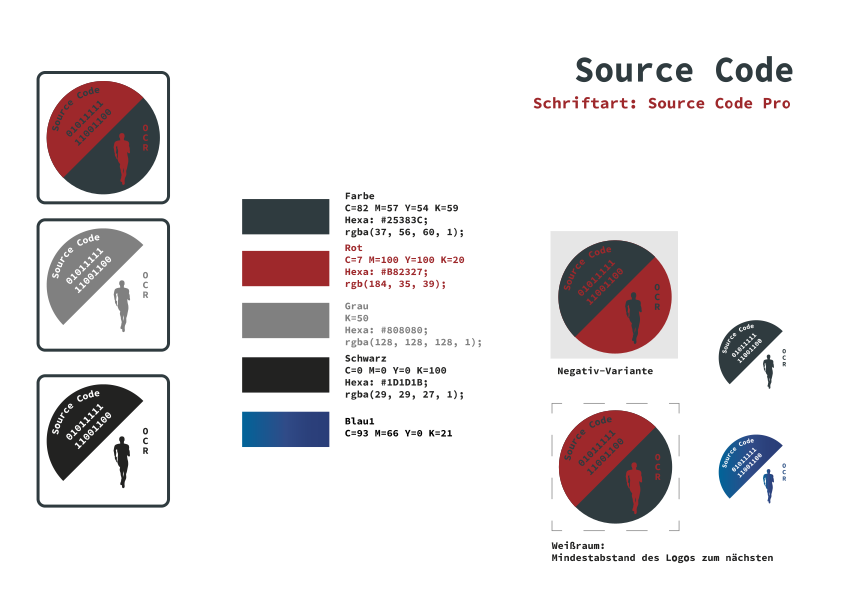
\includegraphics[width=.95\textwidth]{images/Logo-Details.eps}%
	\caption{Abbildung2}\label{fig:Abbildung2}%% anpassen
\end{figure}


Logo in Neg, Grau, Schwarz (\autoref{fig:logoneggrauschwarz}).
%
\begin{figure}[!hb]% hier: !hb
	\centering
	\begin{minipage}[b]{0.40\textwidth}
		
\includegraphics[width=\textwidth]{images/Logo-negativ.eps}%
	\end{minipage}
	\hfill
	\begin{minipage}[b]{0.30\textwidth}
		
\includegraphics[width=\textwidth]{images/Logo-Grau.eps}%
	\end{minipage}
	\hfill
	\begin{minipage}[b]{0.20\textwidth}
		
\includegraphics[width=\textwidth]{images/Logo-SW.eps}%
	\end{minipage}
	\caption{Logo in Neg, Grau, Schwarz}\label{fig:logoneggrauschwarz}%% anpassen
\end{figure}



%\chapter{vorlage-literaturangabe-kfz}
%% letztes Update: 28-Jul-20
\textbf{Zitat -- KFZ}

Quelle: ~\textcite{schmidt:2015:klima}

Quelle: ~\textcite{sternbeck:2015:bremsen}

Quelle: ~\textcite{schneehage:2018:aktoren}

Quelle: ~\textcite{frei:2017:hochvolt}

Quelle: ~\textcite{frei:2013:elektrik}

Quelle: ~\textcite{gunther:2019:commonrail}

Quelle: ~\textcite{peter:2015:benzindirekt}

Quelle: ~\textcite{schneehage:2014:sensoren}

Quelle: ~\textcite{frei:2018:vernetztesysteme}

Quelle: ~\textcite{bosch:2020:training}

%\chapter{vorlage-literaturangabe-sport}
%% letztes Update: 28-Jul-20
\textbf{Zitat -- Sport}

\textbf{Kraft}

Quelle: ~\textcite{lauren:2014:fit90tage}

Quelle: ~\textcite{lauren:2016:fitkraftstoff}

Quelle: ~\textcite{lauren:2017:fit}

\textbf{Laufen}

Quelle: ~\textcite{marquardt:2015:laufbibel}

Quelle: ~\textcite{steffny:2006:laufbuch}

Quelle: ~\textcite{zeller:2017:hindernis}

\textbf{Lauftechnik verbessern}

Quelle: ~\textcite{marquardt:2018:laufstil}

\textbf{Fußtraining}

Quelle: ~\textcite{marquardt:2018:fusstraining}

Quelle: ~\textcite{marquardt:2018:fusstrainingsplan}

\textbf{Trainingsrechner}

\begin{itemize}
\item
  Tempo und die Durchgangszeiten Wettkampf
\item
  Schrittfrequenz
\item
  Zeit/Gewicht
\item
  Lauftempo in Min/km, km/h und m/s umrechnen
\item
  Wettkampfzeit
\item
  Pulsbereiche
\item
  Intervallzeiten
\item
  BMI
\item
  Kalorien/Energie
\end{itemize}

Quelle: ~\textcite{marquardt:2018:trainingsrechner}

\textbf{Trainingspuls finden}

Quelle: ~\textcite{marquardt:2018:pulspace}

\textbf{Trainingspläne für Läufer}

Quelle: ~\textcite{marquardt:2018:trainingsplan5km}

Quelle: ~\textcite{marquardt:2018:trainingsplan10km}

Quelle: ~\textcite{marquardt:2018:trainingsplan21km}

Quelle: ~\textcite{marquardt:2018:trainingsplan42km}

\textbf{Athletik}

Quelle: ~\textcite{marquardt:2018:koordinationstrainingeinsteiger}

Quelle: ~\textcite{marquardt:2018:koordinationstraininglaufen}

Quelle: ~\textcite{marquardt:2018:rueckenuebung}

Quelle: ~\textcite{marquardt:2018:knieuebung}

Quelle: ~\textcite{marquardt:2018:fussuebung}

\textbf{Sport Verletzung}

Quelle: ~\textcite{marquardt:2018:schmerzendesknie}

Quelle: ~\textcite{marquardt:2018:verletzteachilles}

\textbf{Sport Check-up}

Quelle: ~\textcite{marquardt:2018:sportmedizinischertest}

Quelle: ~\textcite{marquardt:2018:bewegungsanalyse}

Quelle: ~\textcite{marquardt:2018:leistungsdiagnostik}

Quelle: ~\textcite{marquardt:2018:laufschuhberatungssysteme}

%\chapter{vorlage-literaturangabe}
%% letztes Update: 28-Jul-20
\textbf{Zitat}

Quelle: ~\textcite{monk:2014:raspberry}

Quelle: ~\textcite{monk:2016:action}

Quelle: ~\textcite{monk:2013:elektronikhacks}

Quelle: ~\textcite{weigend:2018:python}

Quelle: ~\textcite{weigend:2016:raspberry}

Quelle: ~\textcite{schlosser:2016:latex}

Quelle: ~\textcite{homofaciens:2018:projekt}

Quelle: ~\textcite{bartmann:2018:bastelseite}

Quelle: ~\textcite{bartmann:2017:arduino}

Quelle: ~\textcite{joos:2018:windows}

Quelle: ~\textcite{joos:2012:win7}

Quelle: ~\textcite{kofler:2018:infoseite}

Quelle: ~\textcite{kofler:2015:raspberry}

Quelle: ~\textcite{kofler:2017:linux}

Quelle: ~\textcite{kofler:2018:hacking}

Quelle: ~\textcite{kofler:2016:shellbefehle}

Quelle: ~\textcite{kuveler:2009:inf}

Quelle: ~\textcite{loviscach:2018:videos}

Quelle: ~\textcite{riesinger:2017:mathe}

Quelle: ~\textcite{riesinger:2006:inf}

Quelle: ~\textcite{schwichtenberg:2017:ps}

Quelle: ~\textcite{heiderich:2016:technprobleme}

Quelle: ~\textcite{will:2014:einfuehrungcpp}

Quelle: ~\textcite{will:2018:handbuchcpp}

Quelle: ~\textcite{preisel:2017:git}

Quelle: ~\textcite{theis:2017:einstiegcpp}

Quelle: ~\textcite{theis:2017:einstiegc}

Quelle: ~\textcite{theis:2017:einstiegphp}

Quelle: ~\textcite{theis:2017:einstiegpython}

Quelle: ~\textcite{gaicher:2012:programmierenc}

Quelle: ~\textcite{gaicher:2015:avrc}

Quelle: ~\textcite{plotzeneder:2013:powerprojektec}

Quelle: ~\textcite{kuhlee:2012:forensik}

Quelle: ~\textcite{erickson:2008:hacking}

Quelle: ~\textcite{ernesti:2015:python}

